% PAMS: Pre-Aligned Modulus Switching for exact second-order masked ML-KEM ciphertext verification.
% Build: scripts/build.sh (pdflatex + bibtex, TinyTeX). Not submitted to, and not formatted for, any specific venue.
\documentclass[10pt,twocolumn]{article}
\usepackage[letterpaper,margin=0.75in,columnsep=0.25in]{geometry}
\usepackage[T1]{fontenc}
\usepackage{lmodern}
\usepackage{microtype}
\usepackage{amsmath,amssymb,amsthm,mathtools,bm}
\usepackage{graphicx}
\usepackage{booktabs,multirow,tabularx,makecell,threeparttable}
\usepackage{xcolor}
\usepackage{listings}
\usepackage{tikz}
\usetikzlibrary{arrows.meta,positioning,fit,calc,backgrounds,shapes.geometric,decorations.pathreplacing}
\usepackage[font=small,labelfont=bf,skip=4pt]{caption}
\usepackage{subcaption}
\usepackage{enumitem}
\usepackage{siunitx}
\usepackage{float}
\usepackage{stfloats}
\usepackage[numbers,sort&compress]{natbib}
\usepackage[hidelinks]{hyperref}
\usepackage[capitalise,noabbrev]{cleveref}
\usepackage{afterpage}
\usepackage{placeins}

\sisetup{group-separator={,},group-minimum-digits=4}
\newcolumntype{R}[1]{>{\raggedright\arraybackslash}p{#1}}
\newcolumntype{Y}{>{\raggedright\arraybackslash}X}
\setlist{itemsep=1pt,topsep=2pt,leftmargin=*}
\setlength{\textfloatsep}{8pt plus 2pt minus 2pt}
\setlength{\floatsep}{6pt plus 2pt minus 2pt}
\setlength{\dbltextfloatsep}{8pt plus 2pt minus 2pt}

\newtheorem{proposition}{Proposition}
\newtheorem{lemma}{Lemma}
\newtheorem{corollary}{Corollary}
\theoremstyle{definition}
\newtheorem{definition}{Definition}
\newtheorem{example}{Example}
\theoremstyle{remark}
\newtheorem{remark}{Remark}

% ---------------------------------------------------------------- notation (used consistently throughout)
\newcommand{\PAMS}{PAMS}
\newcommand{\Z}{\mathbb{Z}}
\newcommand{\Zq}{\mathbb{Z}_q}
\newcommand{\F}{F_K}
\newcommand{\Fk}[1]{F_{14}\!\left(#1\right)}
\newcommand{\Comp}{\operatorname{Compress}_d}
\newcommand{\Low}{\mathrm{Low}}
\newcommand{\lt}{\mathrm{lt}}
\newcommand{\sig}[1]{\texttt{#1}}
\newcommand{\file}[1]{\texttt{#1}}
\newcommand{\um}{\,\si{\micro\meter\squared}}
\newcommand{\ns}{\,\si{\nano\second}}

% ---------------------------------------------------------------- Verilog listings: verbatim from the frozen RTL
\definecolor{kw}{RGB}{0,0,150}\definecolor{cm}{RGB}{0,110,0}\definecolor{lnum}{RGB}{120,120,120}
\lstdefinestyle{rtl}{language=Verilog,basicstyle=\ttfamily\scriptsize,keywordstyle=\color{kw}\bfseries,
  commentstyle=\color{cm}\itshape,numbers=left,numberstyle=\tiny\color{lnum},numbersep=4pt,breaklines=true,
  breakatwhitespace=false,postbreak=\mbox{\textcolor{lnum}{$\hookrightarrow$}\space},columns=fullflexible,
  keepspaces=true,frame=tb,framerule=0.4pt,xleftmargin=1.2em,aboveskip=4pt,belowskip=2pt,showstringspaces=false}
\lstset{style=rtl}
\newcommand{\RTL}{../final/rtl/pams_jqr.v}
\newcommand{\RTLB}{../final/rtl/base_jq.v}

\title{\Large\bfseries PAMS: Pre-Aligned Modulus Switching for Exact Second-Order Masked\\ ML-KEM Ciphertext Verification in Hardware}
\author{Skyler Lee\\ \small \href{mailto:slee514101@gmail.com}{slee514101@gmail.com}\thanks{Source code, RTL, scripts and the complete evidence trail referenced throughout this paper are public at \url{https://github.com/BlueBrik1/pams}.}}
\date{\today}

\begin{document}
\twocolumn[
\begin{@twocolumnfalse}
\maketitle
\begin{abstract}
\noindent
ML-KEM decapsulation (FIPS~203) re-encrypts the recovered message and accepts the received ciphertext only if the re-encryption matches it exactly. Because this check operates on secret-dependent intermediates, side-channel-protected implementations must evaluate it on masked data. The comparison is not linear in the arithmetic shares, so in hardware it requires protected nonlinear gadgets and a supply of fresh randomness every cycle. We present \PAMS{} (pre-aligned modulus switching), a datapath for the exact masked comparison $\Comp(x) = c$ for all ML-KEM compression widths $d \in \{4,5,10,11\}$.

\PAMS{} combines three published ingredients into a protected datapath that, to our knowledge, has not been described before: share-wise modulus switching with an integer error bound, a precision of $\lceil \log_2(3q) \rceil = 14$ bits, and public interval anchoring with a per-coefficient public threshold. Every share is switched to one fixed 14-bit representation for all four widths. The decision becomes a single masked comparison against a public threshold.

We implement \PAMS{} as a three-share, second-order, HPC2-based RTL lane at one coefficient per cycle. We compare it with the strongest conventional exact lane we could construct, the Simple method with the same gadget, flow and generic optimizations. In Nangate45 synthesis and seeded OpenROAD place-and-route, \PAMS{} needs \num{29.8}\,\% fewer secure gadgets (40 vs.\ 57) and \num{29.8}\,\% fewer fresh random bits per cycle (120 vs.\ 171). The lane (not a complete ML-KEM accelerator) uses \num{19.5}\,\% less routed standard-cell area and \num{18.5}\,\% less estimated die area. Clock periods are comparable; no general speed advantage is demonstrated.

We argue glitch-robust second-order probing security conditionally, under ideal randomness and canonical uniform input sharings. The argument combines SILVER-verified gadgets, the published PINI composition theorem, and netlist-level precondition checks performed by our own structural checker. In focused PROLEAD simulations, no leakage survives confirmation; this is statistical evidence, not a proof. Transition robustness, randomness generation and physical leakage remain open. All results are EDA-tool estimates for a verification subsystem, not silicon measurements.
\end{abstract}

\vspace{1em}
\end{@twocolumnfalse}
]

\section{Introduction}\label{sec:intro}

\paragraph{Post-quantum key establishment.}
The public-key schemes in use today rest on integer factorization and discrete logarithms. A sufficiently large quantum computer would solve both problems efficiently~\cite{shor1997}. Data encrypted today can be recorded now and decrypted later, so the migration to quantum-resistant key establishment must precede such machines. In August 2024 NIST standardized ML-KEM, the Module-Lattice-Based Key-Encapsulation Mechanism derived from CRYSTALS-Kyber, as FIPS~203~\cite{fips203,bos2018kyber}. ML-KEM lets two parties agree on a shared 256-bit secret over a public channel. Its security rests on the module learning-with-errors problem, and it comes in three parameter sets: ML-KEM-512, -768 and -1024.

\paragraph{Re-encryption checking.}
ML-KEM obtains security against chosen-ciphertext attacks (IND-CCA2) from a variant of the Fujisaki--Okamoto transform~\cite{fujisaki1999,hofheinz2017}. Decapsulation decrypts the ciphertext, re-encrypts the recovered message deterministically, and compares the result with the received ciphertext. Only if every coefficient matches is the real shared key released; otherwise an implicit-rejection key is returned. The comparison is \emph{exact}: it must reject any ciphertext that differs in even one compressed coefficient.

\paragraph{Why the check must be protected.}
The re-encrypted ciphertext depends on the secret key. An adversary who can observe power or electromagnetic leakage, and who submits manipulated ciphertexts, can turn the success or failure of the check into an oracle on secret data. Generic side-channel attacks of this kind on CCA-secure lattice KEMs have been demonstrated~\cite{ravi2020}. Hardened implementations therefore \emph{mask} the computation. Each sensitive value $x$ is split into $n$ random shares whose sum (or XOR) equals $x$, and every intermediate value is computed on shares. Any $n-1$ observed intermediates are then statistically independent of $x$~\cite{ishai2003}. With $n = 3$ shares the implementation is \emph{second-order} masked.

\paragraph{Why exact masked comparison is expensive.}
In masked ML-KEM the re-encrypted coefficients are naturally available as \emph{arithmetic} shares modulo $q = 3329$. Checking them against the public ciphertext needs the compression function $\Comp$, a rounding of $2^d x/q$, followed by an equality test. Neither operation is linear in arithmetic shares mod $q$. Exact masked methods therefore convert to Boolean shares and evaluate an adder or comparator on them~\cite{bos2021masking,fritzmann2022,danvers2023,coron2023poly}. In hardware every nonlinear Boolean operation on shares must be a protected \emph{gadget}, such as HPC2~\cite{cassiers2021hpc}, which costs registers, area and fresh randomness. Pipelined at one coefficient per cycle, a second-order HPC2 gadget needs three fresh random bits per cycle, and in our flow it occupies about $180\um$. The number of gadgets thus directly sets the area of the verification lane and the bandwidth demanded from the random-number generator.

\paragraph{The gap.}
The strongest exact conventional method we found, the "Simple" approach of Fritzmann et al.\ and D'Anvers et al.~\cite{fritzmann2022,danvers2023}, switches every share to a power-of-two modulus with $d + 13$ bits. For ML-KEM-1024 ($d = 11$) the protected adder is therefore 24 bits wide. Coron et al.'s HOCompress~\cite{coron2023poly} uses 14 extra bits on top of the $d$ integer bits. Interval-based methods (Bos et al., Azouaoui et al.~\cite{bos2021masking,azouaoui2023}) avoid that width but need exact prime-modulus conversions. We found no published construction that removes the dependence of the protected width on $d$ while remaining exact.

\paragraph{This work.}
\PAMS{} combines three established mechanisms:
\begin{itemize}
  \item the integer-error share-wise modulus switch of Coron, G\'erard, Trannoy and Zeitoun~\cite{coron2023dil};
  \item the precision rule $\lceil \log_2(nq) \rceil$ of HOCompress~\cite{coron2023poly};
  \item the integer interval anchoring and public-threshold comparison of Bos et al.\ and Azouaoui et al.~\cite{bos2021masking,azouaoui2023}.
\end{itemize}
Each share is switched to one fixed 14-bit representation for every $d$. The public interval start of $c$ is subtracted on one share, and the masked sum is compared with a per-coefficient public threshold $\Theta_c$. The protected datapath becomes 14 bits wide for all ML-KEM parameter sets. This saves 17 of 57 gadgets relative to the Simple lane built from the same parts.

\paragraph{Contributions.}
\begin{enumerate}
  \item \textbf{Datapath.} An exact masked ML-KEM ciphertext-coefficient verification datapath (\cref{sec:math}). It combines share-wise modulus switching into a fixed 14-bit representation with public interval anchoring and a per-coefficient threshold comparison, for $d \in \{4,5,10,11\}$. The mathematical components are published; to our knowledge, their combination for exact ML-KEM verification has not been described before (\cref{sec:related}).
  \item \textbf{Implementation.} A complete three-share HPC2 RTL implementation at one coefficient per cycle, explained from equations to registers (\cref{sec:rtl,app:verilog}).
  \item \textbf{Physical realization.} Gate-level and placed-and-routed evidence from real netlists and layouts (\cref{sec:circuit,app:circuit}).
  \item \textbf{Matched evaluation.} A comparison against the strongest conventional exact lane we could build, with fairness controls and seeded physical design (\cref{sec:method,sec:results}). Across seven seeds and three clock targets, the \PAMS{} lane reduces routed cell area of the verification lane by \num{19.5}\,\% and gadgets and randomness by \num{29.8}\,\%, at comparable clock period.
  \item \textbf{Security evidence and its limits.} The evidence is stated in the glitch-robust probing model (\cref{sec:security}), and the open questions are stated explicitly (\cref{sec:limits}).
\end{enumerate}

\paragraph{Organization.}
\begin{itemize}
  \item \Cref{sec:background} reviews ML-KEM compression, masking and the related work.
  \item \Cref{sec:arch} develops \PAMS{} in three layers: the mathematics, the Verilog, and the circuit with its physical realization.
  \item \Cref{sec:security} analyses security, \cref{sec:method} describes the experimental methodology, and \cref{sec:results} reports the results.
  \item \Cref{sec:limits,sec:conclusion} discuss limitations and conclude.
  \item The appendices give the complete derivations (\cref{app:math}), an annotated walkthrough of the Verilog (\cref{app:verilog}) and of the gate-level and physical circuit (\cref{app:circuit}), and extended security and experimental evidence (\cref{app:evidence}).
\end{itemize}

\section{Background}\label{sec:background}

\subsection{ML-KEM arithmetic and ciphertext compression}\label{sec:mlkem}
ML-KEM computes in the ring $R_q = \Zq[X]/(X^{256}+1)$ with the prime $q = 3329$~\cite{fips203}.
\begin{itemize}
  \item A polynomial has 256 coefficients in $\Zq = \{0, 1, \dots, q-1\}$, and addition and multiplication of coefficients are modulo $q$.
  \item A ciphertext consists of $k$ polynomials $\mathbf u$ and one polynomial $v$, with $k = 2, 3, 4$ for ML-KEM-512/768/1024.
  \item To shorten the ciphertext, every coefficient is \emph{compressed} to $d$ bits: $d_u = 10, 10, 11$ for $\mathbf u$ and $d_v = 4, 4, 5$ for $v$.
\end{itemize}

The four widths that occur are therefore $d \in \{4, 5, 10, 11\}$.

\paragraph{Compression.} FIPS~203 defines, for $x \in \Zq$,
\begin{equation}\label{eq:compress}
  \Comp(x) \;=\; \Bigl\lceil \tfrac{2^d}{q}\, x \Bigr\rfloor \bmod 2^d
  \;=\; \Bigl\lfloor \tfrac{2^{d+1} x + q}{2q} \Bigr\rfloor \bmod 2^d ,
\end{equation}
where $\lceil\cdot\rfloor$ rounds to the nearest integer with ties rounded up. The integer form on the right is the one the reference model uses (\file{models/pams.py}). Because $q$ is odd, $2^{d+1}x/q$ is never an odd integer for $x \in \Zq$, so no tie can occur. Decompression maps $y \in [0, 2^d)$ to $\lceil q y / 2^d \rfloor$.

\paragraph{Compression intervals.} For fixed $d$, $\Comp$ is a non-decreasing step function on $\{0, \dots, q-1\}$ followed by a reduction mod $2^d$. Each value $c \in [0, 2^d)$ is therefore taken on a cyclic interval of $\Zq$:
\begin{equation}\label{eq:interval}
\begin{aligned}
  \Comp(x) = c &\iff x \in I_c = [a_c, a_{c+1}) \ \text{(cyclically)},\\
  a_c &= \Bigl\lceil \tfrac{(2c-1)\,q}{2^{d+1}} \Bigr\rceil \bmod q .
\end{aligned}
\end{equation}
\Cref{app:math-intervals} derives \cref{eq:interval}. The interval for $c = 0$ wraps around zero: for $d = 4$, $I_0 = \{3225, \dots, 3328, 0, \dots, 104\}$. The interval widths are $\{208, 209\}$, $\{104, 105\}$, $\{3, 4\}$ and $\{1, 2\}$ for $d = 4, 5, 10, 11$.

\paragraph{The verification predicate.}
During decapsulation, the re-encryption produces coefficients $x$ of $\mathbf u'$ and $v'$, and the received ciphertext supplies compressed coefficients $c$. The check is
\begin{equation}\label{eq:pred}
  D \;=\; \bigwedge_{\text{all coefficients}} \bigl[\, \Comp(x) = c \,\bigr] ,
\end{equation}
where the conjunction runs over $256(k+1)$ coefficients with the appropriate $d$ per polynomial. $D = 1$ selects the real shared key and $D = 0$ the implicit-rejection key. The coefficient $c$ is public, but $x$ and $D$ are sensitive until the selection has been made.

\subsection{Masking}\label{sec:masking}
\paragraph{Shares.} Masking splits a sensitive value into $n$ shares whose combination equals it:
\begin{itemize}
  \item \emph{arithmetic} shares mod $q$: $x = x_0 + x_1 + x_2 \bmod q$, each $x_i \in \Zq$;
  \item \emph{Boolean} shares: $b = b_0 \oplus b_1 \oplus b_2$.
\end{itemize}

In a uniform sharing any $n-1$ shares are jointly uniform and independent of the secret. With $n = 3$ an adversary who observes two shares learns nothing.

\emph{Example.} $x = 3300$ can be shared as $(487, 1308, 1505)$: $487 + 1308 + 1505 = 3300$. Any two of the three numbers are uniformly distributed when the sharing is chosen at random.

\paragraph{Linear and nonlinear operations.} Adding a public constant to one share, adding two sharings share-wise, or XOR-ing Boolean sharings are \emph{share-local} (linear) operations. Each output share depends on one input share, so they cost no randomness and no extra security reasoning. A nonlinear operation such as the AND $c = a \wedge b$ of two Boolean sharings needs the cross products $a_i b_j$ for $i \ne j$. Those must be re-randomized with fresh random bits and separated by registers, or a single probe could combine information from two shares. Converting an arithmetic sharing into a Boolean one (A2B) or comparing a masked value needs Boolean addition. Boolean addition is nonlinear (carries are AND/majority functions), and it is the dominant cost of every exact masked comparison.

\paragraph{Probing model and glitches.} In the $t$-probing model~\cite{ishai2003} the adversary observes the values of $t$ wires; $t = 2$ for second order with three shares. In hardware a combinational wire can glitch and briefly expose any input of its logic cone. The \emph{glitch-robust} probing model~\cite{faust2018} therefore extends each probe to all register outputs and primary inputs that feed the probed wire combinationally in that cycle. \emph{Transitions}, the leakage of consecutive values on one wire or register, form a further model~\cite{cassiers2021trans}.

\paragraph{HPC2 and PINI.} Probe-Isolating Non-Interference (PINI)~\cite{cassiers2020pini} is a gadget property: any $t$ probes inside a gadget can be simulated with at most $t$ input-share indices, the same indices as the probes' own share domains. A circuit built only from PINI gadgets, in which every wire stays in one share domain outside gadgets, is itself PINI. This is \emph{trivial composition}. HPC2~\cite{cassiers2021hpc} is a glitch-robust PINI AND gadget for any order:
\begin{itemize}
  \item for three shares it consumes $\binom{3}{2} = 3$ fresh random bits per execution;
  \item it has a latency of two clock cycles;
  \item it can start a new execution every cycle.
\end{itemize}

Its structure is shown in \cref{app:hpc2}. In this work every nonlinear operation on masked data is one HPC2 AND; majority, OR and comparator steps are expressed through it.

\subsection{Related work}\label{sec:related}
\paragraph{Exact masked ciphertext comparison.}
\begin{itemize}
  \item \textbf{Bos et al.}~\cite{bos2021masking} anchor the comparison at the integer interval of \cref{eq:interval}. They perform two range checks per coefficient, each the most significant bit of an exact arithmetic-to-Boolean conversion \emph{modulo $q$}.
  \item \textbf{Fritzmann et al.}~\cite{fritzmann2022} compute a masked $\Comp$ by switching every share to $2^{d+f}$ with $f$ fractional bits, converting to Boolean, and dropping the fractional bits.
  \item \textbf{D'Anvers et al.}~\cite{danvers2022,danvers2023} generalize the methods into a framework of pre-processing, A2B and post-processing. Their exact "Simple" method subtracts the scaled compressed value and tests the top $d$ bits for zero. Their faster hybrid and Galois-field methods accept a collision probability and are therefore not exact.
  \item \textbf{Coron et al.}~\cite{coron2023poly} give HOCompress, a modulus switch to $2^{d+\alpha}$ with $\alpha = \lceil \log_2(qn) \rceil$ followed by A2B, and arithmetic zero tests. Their multi-coefficient batching uses random linear combinations, which again are not exact.
  \item \textbf{Coron, G\'erard, Trannoy and Zeitoun}~\cite{coron2023dil} (Dilithium) state the share-wise switching lemma that \PAMS{} uses: the floor-sum of the shares differs from the switched secret by an integer error $0 \le e \le n-1$.
  \item \textbf{Azouaoui et al.}~\cite{azouaoui2023} compare a masked value with a public bound through a carry-only adder (SecLeq) after an exact mod-$q$ conversion.
\end{itemize}

\paragraph{Conversion hardware.} Norga et al.~\cite{norga2024x2x} and Shahmirzadi and Hutter~\cite{shahmirzadi2024} design A2B/B2A hardware. X2X uses Brent--Kung adders and, for its largest savings, DOM gadgets with explicit refresh~\cite{gross2016dom}, a different composition model from PINI. Bronchain and Cassiers~\cite{bronchain2022} bitslice conversions in software.

\paragraph{Masked ML-KEM hardware.}
\begin{itemize}
  \item Kamucheka et al.~\cite{kamucheka2022} present a first-order FPGA design.
  \item HOPE-MLKEM~\cite{camacho2026hope} provides a configurable high-order design. In the released RTL we inspected, its comparison path recombines shares before compression.
  \item Buschkowski et al.~\cite{buschkowski2026} automate mixed-domain masking for an arbitrary-order ML-KEM core. We could read only the abstract, which does not describe the comparison.
  \item Ranney et al.~\cite{ranney2026} implement a higher-order masked comparison on FPGA and report first-order leakage due to parallelism.
  \item Hermelink et al.~\cite{hermelink2024} show that $t$-probing security of the FO comparison is not sufficient in practice against vertical attacks.
\end{itemize}

\paragraph{What \PAMS{} takes and what it adds.}
\PAMS{} takes from prior work:
\begin{itemize}
  \item the switching lemma~\cite{coron2023dil};
  \item the precision $\lceil \log_2 (3q) \rceil = 14$~\cite{coron2023poly};
  \item the integer interval anchor~\cite{bos2021masking};
  \item the public-threshold comparison~\cite{azouaoui2023}.
\end{itemize}

What it combines differently is the following. A \emph{single} $d$-independent 14-bit switch of the shares is anchored at the integer interval start, and the decision is one threshold comparison whose public threshold depends on $(c, d)$. This replaces both the $d$-dependent block test of Simple/HOCompress ($d + 13$ or $d + 14$ bits) and the prime-modulus conversions of Bos and Azouaoui. Fritzmann et al.\ explicitly consider interval comparison and set it aside for $d \ge 2$~\cite[\S2.2.3]{fritzmann2022}; the per-coefficient threshold is what removes that obstacle. We make no claim of a new mathematical identity: exactness follows from the published lemma in a few lines (\cref{sec:exact}).

\paragraph{Choice of baseline.}
\begin{itemize}
  \item In the comparison of D'Anvers et al.~\cite{danvers2023}, the Simple method is the fastest \emph{exact} method.
  \item In our own hardware study (\cref{sec:method}), it was also the strongest family. Bos-style interval checking, HOCompress precision and Brent--Kung prefix carries all gave larger lanes. The Coron arithmetic zero test is bounded from below by more area than the whole \PAMS{} lane (\cref{app:competitors}).
  \item We therefore compare against the best Simple lane we could build. It is not claimed to be optimal among all possible circuits.
\end{itemize}

\section{PAMS Architecture}\label{sec:arch}

This section develops \PAMS{} in three layers. \Cref{sec:math} derives the decision predicate and proves it exact. \Cref{sec:rtl} shows how the final RTL, \file{final/rtl/pams\_jqr.v}, computes each term. \Cref{sec:circuit} follows the RTL into synthesized gates and the placed-and-routed layout.

The design evaluated throughout is \sig{pams\_jqr}. It is the frozen \PAMS{} algorithm of the original design \sig{pams} with three implementation-level changes, none of which changes the decision function:
\begin{itemize}
  \item just-in-time operand delays;
  \item a two-stage share-wise multiplier;
  \item retimed public logic.
\end{itemize}

\subsection{Mathematical Construction}\label{sec:math}

\paragraph{A.~The exact problem.}
One coefficient is verified per clock cycle. The circuit receives:
\begin{itemize}
  \item three \emph{canonical} arithmetic shares $x_0, x_1, x_2 \in \{0, \dots, q-1\}$ of the re-encrypted coefficient $x = x_0 + x_1 + x_2 \bmod q$;
  \item the public received compressed coefficient $c \in [0, 2^d)$;
  \item the public width $d \in \{4, 5, 10, 11\}$.
\end{itemize}
It must output a three-share Boolean sharing of
\begin{equation}\label{eq:target}
  b \;=\; \bigl[\, \Comp(x) = c \,\bigr] \in \{0,1\},
\end{equation}
and, over a ciphertext, a sharing of $D = \bigwedge b$ (\cref{eq:pred}). Neither $x$ nor $b$ may be recombined.

A direct approach computes a masked $\Comp(x)$ (a $d$-bit Boolean sharing) and then tests equality with $c$. In hardware the masked compression is itself a modulus switch plus a Boolean adder whose width grows with $d$, as in Simple and HOCompress. The equality is a further $d$-bit zero test. \PAMS{} never forms $\Comp(x)$. It asks directly whether $x$ lies in the public interval $I_c$, and it formulates that question so that the protected adder has the same small width for every $d$.

\paragraph{B.~Notation.} The following symbols are used throughout the paper.
\begin{center}\footnotesize
\begin{tabularx}{\columnwidth}{@{}>{\raggedright\arraybackslash}p{3.0cm}X@{}}
\toprule
symbol & meaning \\
\midrule
$q = 3329$, $n = 3$ & modulus; number of shares \\
$d \in \{4,5,10,11\}$ & compression width (per coefficient) \\
$x_i$, $x$ & canonical shares; $x = \sum x_i \bmod q$ \\
$c \in [0, 2^d)$ & public compressed coefficient \\
$K = 14$ & width of the switched representation \\
$F_K(v) = \lfloor 2^K v / q \rfloor$ & modulus switch (any integer $v$) \\
$y_i = F_K(x_i)$ & switched share $i$ (secret, domain $i$) \\
$j \in \{0,1,2\}$ & integer switching error, \cref{eq:lemma} \\
$a_c$; $I_c = [a_c, a_{c+1})$ & public interval of $c$, \cref{eq:interval} \\
$\Low_c = F_K(a_c) \bmod 2^K$ & public anchor \\
$\Theta_c$ & public threshold, \cref{eq:theta} \\
$\hat y_0 = y_0 + 2 - \Low_c$ & anchored share 0 (mod $2^K$) \\
$Z = \hat y_0 + y_1 + y_2$ & masked switched offset (mod $2^K$) \\
$b = [Z < \Theta_c]$ & per-coefficient decision \\
$g$ & minimum gap of $F_K$, \cref{eq:gap} \\
\bottomrule
\end{tabularx}
\end{center}
All arithmetic on $y_i$, $\Low_c$, $\Theta_c$ and $Z$ is modulo $2^K$, i.e.\ on 14-bit words.

\paragraph{C.~Share-wise modulus switching.}
A power-of-two modulus is what hardware adds natively: a $K$-bit adder computes sums mod $2^K$ by discarding the carry out. Mod $q$, by contrast, needs a comparison and a conditional subtraction. Masked Boolean addition is the expensive part of every exact comparison, so we want it to happen mod $2^K$ with small $K$.

The map $F_K$ is applied to each share separately. This is share-local: domain $i$ computes $y_i = F_K(x_i)$ from its own share with a constant multiplier, and no other domain is involved. The sum of the switched shares is close to the switched secret.
\begin{lemma}[integer-error switching; Coron et al.~\cite{coron2023dil}, Lemma~2]\label{lem:switch}
For canonical shares $x_0, \dots, x_{n-1} \in [0, q)$ with $x = \sum x_i \bmod q$,
\begin{equation}\label{eq:lemma}
  \sum_{i} F_K(x_i) \;\equiv\; F_K(x) - j \pmod{2^K}
\end{equation}
for some integer $j \in \{0, 1, \dots, n-1\}$.
\end{lemma}
\begin{proof}
\emph{Step 1 (one share).} Write $2^K x_i = q F_K(x_i) + r_i$ with remainder $r_i \in [0, q)$. Summing over $i$,
\[ q \textstyle\sum_i F_K(x_i) = 2^K \sum_i x_i - \sum_i r_i . \]

\emph{Step 2 (the secret).} Since $\sum_i x_i = x + kq$ with $k \in \{0, \dots, n-1\}$ and $2^K x = q F_K(x) + r$ with $r \in [0, q)$, we have
\[ q \textstyle\sum_i F_K(x_i) = q F_K(x) + r + 2^K k q - \sum_i r_i . \]

\emph{Step 3 (remainders).} Reducing mod $q$ shows $\sum_i r_i \equiv r \pmod q$. Because $0 \le \sum_i r_i \le n(q-1)$, we get $\sum_i r_i = r + jq$ for an integer $j$ with $0 \le j \le n - 1$.

\emph{Step 4.} Substituting and dividing by $q$ gives $\sum_i F_K(x_i) = F_K(x) - j + 2^K k$, which is \cref{eq:lemma}.
\end{proof}
The error $j$ is secret and unknown. It depends on the shares, not only on $x$. For $K = 14$, $j = 2$ occurs for 3,327 of the 3,329 values of $x$; Phase XII enumerated all $3329^3 = \num{36892780289}$ canonical triples with 0 violations. \PAMS{} absorbs the error by a public offset of $n - 1 = 2$ (the same offset as ModSwitch~\cite{coron2023dil}): $\sum F_K(x_i) + 2 = F_K(x) + (2 - j)$ with $2 - j \in [0, 2]$. The decision is then chosen so that an error in $[0, 2]$ can never move a value across a decision boundary.

\paragraph{D.~Interval anchors and thresholds.}
By \cref{eq:interval}, $b = 1$ iff $x \in [a_c, a_{c+1})$ cyclically. Rather than testing two bounds, \PAMS{} moves the interval start to zero. The anchor $\Low_c = F_K(a_c)$ is subtracted, and the interval end becomes the single public threshold
\begin{equation}\label{eq:theta}
  \Theta_c \;=\; F_K(a_{c+1}) - F_K(a_c) - 1 \pmod{2^K}.
\end{equation}
Both depend only on the public pair $(c, d)$. The RTL evaluates them through closed forms. With $e = 13 - d$, $r_c = ((1 - 2c)\,q) \bmod 2^{d+1}$ and $\mathrm{qq}(r) = \lfloor r\,2^{e}/q \rfloor \in [0, 4]$ (derived in \cref{app:math-anchors}):
\begin{align}
  \Low_c &= (2c - 1)\, 2^{e} + \mathrm{qq}(r_c) \pmod{2^{14}}, \label{eq:low}\\
  \Theta_c &= 2^{e+1} - 1 + \mathrm{qq}(r_{c+1}) - \mathrm{qq}(r_c), \label{eq:thetaclosed}
\end{align}
where $r_{c+1} = (r_c - 2q) \bmod 2^{d+1}$.
Over all 3,120 pairs $(c, d)$, $3 \le \Theta_c \le 1027 < 2^{11}$.

\emph{Wraparound.} The interval $I_0$ wraps through $q - 1 \to 0$; for $d = 4$, $a_0 = 3225$ and $a_1 = 105$. Arithmetic mod $2^K$ handles this without a special case. $F_K$ satisfies $F_K(v + q) = F_K(v) + 2^K$, so the switched positions of $\Zq$ lie on a circle of circumference $2^K$, just as $\Zq$ itself is a circle of circumference $q$. Subtracting $\Low_c$ mod $2^K$ rotates that circle so that $I_c$ starts at 0.

\paragraph{E.~The complete predicate.} From arithmetic shares to the protected decision:
\begin{align}
  y_i &= F_K(x_i) = (x_i \cdot 10321339) \gg 21 , \label{eq:yi}\\
  \hat y_0 &= y_0 + 2 - \Low_c \bmod 2^{14} , \label{eq:y0}\\
  Z &= \hat y_0 + y_1 + y_2 \bmod 2^{14} , \label{eq:Z}\\
  b &= [\, Z < \Theta_c \,] . \label{eq:b}
\end{align}
\Cref{eq:yi} is computed share-wise on secret data. \Cref{eq:y0} touches share 0 only and adds the public $\Low_c$. \Cref{eq:Z} is the masked three-operand sum, and \cref{eq:b} the masked comparison with the public $\Theta_c$.
The multiplier constant $M = 10321339$ and shift $21$ give $\lfloor x_i 2^{14}/q \rfloor$ exactly for every $x_i \in [0, q)$ (Phase XII check B).

\emph{Public versus secret terms.}
\begin{itemize}
  \item \emph{Public:} $\Low_c$, $\Theta_c$ and every bit of them.
  \item \emph{Secret:} each $y_i$ is known only to domain $i$, and no domain ever holds $Z$, $j$ or $b$ in the clear.
  \item \emph{Where the sharing is converted:} \cref{eq:Z,eq:b} are evaluated on a Boolean sharing in which $y_i$ is share $i$ and the other two shares are zero. A carry-save adder (CSA) reduces the three operands to two. A ripple carry chain then computes $Z$ bit by bit, and a ripple comparator against the public bits of $\Theta_c$ runs alongside it.
\end{itemize}
Because $\Theta_c$ is public, each comparator step costs one AND gadget, and all negations of $\Theta_c$ bits are applied to share 0 for free. Because $\Theta_c < 2^{11}$, the comparator splits: $b = [Z_{13:11} = 0] \wedge [Z_{10:0} < \Theta_{c,10:0}]$. The top three bits need only a carry-free zero test. \Cref{tab:kernel} lists the resulting gadget budget next to the Simple baseline.

\begin{table}[t]\centering\small
\caption{HPC2 gadgets per lane by function (counted in the RTL; identical in every mapped netlist).}\label{tab:kernel}
\begin{tabular}{@{}lrr@{}}
\toprule
part & \PAMS{} & Simple baseline \\
\midrule
CSA majorities (3 operands $\to$ 2) & 13 & 23 \\
ripple carries & 10 & 12 \\
comparator against $\Theta_c$ & 10 & -- \\
top region (zero test, OR tree) & 4 & 20 \\
final combination & 1 & 0 \\
ciphertext accumulator & 2 & 2 \\
\midrule
\textbf{total} & \textbf{40} & \textbf{57} \\
fresh random bits per cycle ($3 \times$) & 120 & 171 \\
masked operand width & 14 bit & 24 bit \\
\bottomrule
\end{tabular}
\end{table}

\paragraph{F.~Exactness.}\label{sec:exact}
The proof uses one property of $F_K$: consecutive switched values are at least $g$ apart, where
\begin{equation}\label{eq:gap}
  g \;=\; \min_{v \in \Z}\bigl(F_K(v+1) - F_K(v)\bigr) = \lfloor 2^K/q \rfloor .
\end{equation}
For $K = 14$, $2^{14}/q = 4.92$, so $g = 4$ and every step of $F_{14}$ is 4 or 5. This holds also across the wrap, since $2^{14} - F_{14}(q-1) = 5$. For $K = 13$, $g = 2$.

\begin{proposition}[exactness of \PAMS{}]\label{prop:exact}
Let $K = 14$, $d \in \{4,5,10,11\}$, $c \in [0, 2^d)$ and canonical shares $x_0, x_1, x_2 \in [0, q)$ of $x$. Define $Z$ by \cref{eq:yi,eq:y0,eq:Z} and $\Theta_c$ by \cref{eq:theta}. Then $[Z < \Theta_c] = [\Comp(x) = c]$. More precisely, members satisfy $0 \le Z \le \Theta_c - 1$, and non-members satisfy $\Theta_c + 1 \le Z \le 2^{14} - 2$.
\end{proposition}
\begin{proof}
\emph{Setup.} By \cref{lem:switch}, $Z \equiv F_K(x) - F_K(a_c) + (2 - j) \pmod{2^K}$ with $2 - j \in [0, 2]$.
\begin{itemize}
  \item Let $\tilde x$ be the representative of $x$ in $[a_c, a_c + q)$ and $\tilde a$ that of $a_{c+1}$ in $(a_c, a_c + q]$.
  \item Quasi-periodicity gives $F_K(\tilde x) \equiv F_K(x)$, so $Z \equiv \Delta + (2 - j)$ with $\Delta = F_K(\tilde x) - F_K(a_c) \in [0, 2^K)$.
  \item Put $D_c = F_K(\tilde a) - F_K(a_c)$. Since $0 < D_c < 2^K$, $\Theta_c = D_c - 1$ as an integer.
\end{itemize}

\emph{Members} ($a_c \le \tilde x \le \tilde a - 1$). Here $0 \le \Delta \le F_K(\tilde a - 1) - F_K(a_c) \le D_c - g$, so $0 \le \Delta + 2 - j \le D_c - g + 2 = \Theta_c + 3 - g$. With $g = 4$ this is at most $\Theta_c - 1 < 2^K$: no wrap occurs, and $Z < \Theta_c$.

\emph{Non-members} ($\tilde a \le \tilde x \le a_c + q - 1$). Here $\Delta \ge D_c$, and $\Delta \le F_K(a_c + q - 1) - F_K(a_c) \le 2^K - g$. Hence $\Theta_c + 1 = D_c \le \Delta + 2 - j \le 2^K - g + 2 = 2^K - 2$. Again no wrap occurs, and $Z \ge \Theta_c$.
\end{proof}
The bounds are tight. Evaluating every $(x, j, c, d)$ for this paper gives $\max(Z - \Theta_c) = -1$ over members and $\min(Z - \Theta_c) = +1$ over non-members. Phase XII's exhaustive check of the decision rule over all $3329 \cdot 3 \cdot (2^4 + 2^5 + 2^{10} + 2^{11})$ cases found 0 mismatches. Together with \cref{lem:switch}, that enumeration is a second, computational proof for the stated input contract, assuming the enumeration script is correct (\cref{app:math-exact}). This review re-ran the bound check (\file{paper/scripts/audit\_math.py}), but did not repeat the $3329^3$ lemma enumeration.

\begin{remark}[scope of the 14-bit requirement]\label{rem:k13}
The proof needs $g \ge 4$ for the chosen offset and threshold. Any exact rule on $Z$ needs $g \ge 3$, because an error range of width 3 must fit between neighbouring switched values. The first $K$ with $\lfloor 2^K/q \rfloor \ge 3$ is $K = 14$. At $K = 13$ ($g = 2$), members and non-members collide on \emph{reachable} share triples for every $d$. For example, at $d = 11$, $x = 0$ shared as $(0, 0, 0)$ and $x = 1$ shared as $(3326, 2, 2)$ give the same switched sum. So no decision function of $Z$ can be exact.

This lower bound holds \emph{only in the share-wise floor model}, where $y_i = \lfloor 2^K x_i/q \rfloor$ and the decision depends only on $\sum y_i$ plus public offsets. It is not a lower bound for all masked circuits: other conversions (prime-modulus A2B, rounding with share-dependent offsets) are outside it.
\end{remark}

\emph{Canonical shares.} The proof is stated for canonical shares $x_i < q$, and the hardware is verified only for them. Two facts bound what happens outside that range.
\begin{itemize}
  \item The proof of \cref{lem:switch} does not itself use $x_i < q$: it holds for any non-negative integer shares.
  \item The 12-bit constant multiplier equals $F_{14}$ (mod $2^{14}$) on every 12-bit input except $x_i = 3329$ and $x_i = 4005$, where it is one too small.
\end{itemize}
Our review searched non-canonical inputs only by sampling and found no wrong decision, but it did not analyse them completely. Such inputs would affect correctness, not masking. Neither \PAMS{} nor the baseline checks its inputs, so canonical shares are an interface requirement on the upstream masked re-encryption, for both designs alike.

\paragraph{G.~Worked examples.} \Cref{tab:examples} traces four coefficients through \cref{eq:yi,eq:y0,eq:Z,eq:b}.
\begin{itemize}
  \item \textbf{Source:} every value was computed by the reference model (\file{models/pams.py}). It was then \emph{independently} read back from the internal registers of the simulated final RTL (\file{paper/scripts/examples.py}); the two agree exactly.
  \item \textbf{E1} is a member of the wrapped interval $I_0$ at $d = 4$.
  \item \textbf{E2} is the first value of the next interval at $d = 11$, with the worst-case error $j = 2$. It is rejected with the minimum possible margin, $Z = \Theta_c + 1$.
  \item \textbf{E3} is the last member of its interval at $d = 10$.
  \item \textbf{E4} lies just before the start of $I_0$ and wraps to $Z = 2^{14} - 5$.
\end{itemize}

\begin{table*}[t]\centering\small
\caption{Worked examples (all values mod $2^{14}$ unless stated). Shares and every intermediate quantity were verified against the internal registers of the simulated \sig{pams\_jqr} RTL: \sig{x$i$r}, \sig{s$i$p} ($=y_i$), \sig{y0} ($=\hat y_0$), \sig{lowp} ($=\Low_c$), \sig{th2} ($=\Theta_c$), and the recombined \sig{cdec} at stage~31.}\label{tab:examples}
\setlength{\tabcolsep}{3pt}
\resizebox{\textwidth}{!}{%
\begin{tabular}{@{}lrrrrrrrrrrrrrr@{}}
\toprule
 & $x$ & $(x_0, x_1, x_2)$ & $d$ & $c$ & $\Comp(x)$ & $[a_c, a_{c+1})$ & $F_{14}(x)$ & $(y_0, y_1, y_2)$ & $j$ & $\Low_c$ & $\Theta_c$ & $\hat y_0$ & $Z$ & $b$ \\
\midrule
E1 & 3300 & (487, 1308, 1505) & 4 & 0 & 0 & [3225, 105) & 16241 & (2396, 6437, 7407) & 1 & 15872 & 1027 & 2910 & 370 & 1 \\
E2 & 1627 & (1722, 3208, 26) & 11 & 1000 & 1001 & [1625, 1627) & 8007 & (8474, 15788, 127) & 2 & 7997 & 9 & 479 & 10 & 0 \\
E3 & 976 & (2345, 2243, 3046) & 10 & 300 & 300 & [974, 977) & 4803 & (11541, 11039, 14991) & 0 & 4793 & 14 & 6750 & 12 & 1 \\
E4 & 3224 & (3076, 3166, 311) & 4 & 0 & 15 & [3225, 105) & 15867 & (15138, 15581, 1530) & 2 & 15872 & 1027 & 15652 & 16379 & 0 \\
\bottomrule
\end{tabular}}
\end{table*}

For E1, step by step:
\begin{itemize}
  \item Share-wise switching gives $y = (2396, 6437, 7407)$, whose sum is $16240 \equiv F_{14}(3300) - 1$. Hence $j = 1$.
  \item Share 0 is anchored to $\hat y_0 = 2396 + 2 - 15872 \equiv 2910$.
  \item The masked sum is $Z = 2910 + 6437 + 7407 = 16754 \equiv 370$.
  \item $370 < \Theta_0 = 1027$, so $b = 1$, and indeed $\Comp(3300) = 0$.
\end{itemize}
In E4 the switched sum lands just \emph{below} the anchor. The subtraction wraps to $Z = 16379$, far above $\Theta_0$, which is the cyclic behaviour that removes any special case for $I_0$. \Cref{fig:boundaries} plots $Z$ against $x$ at both ends of $I_0$ for all three values of $j$.

\begin{figure*}[t]\centering
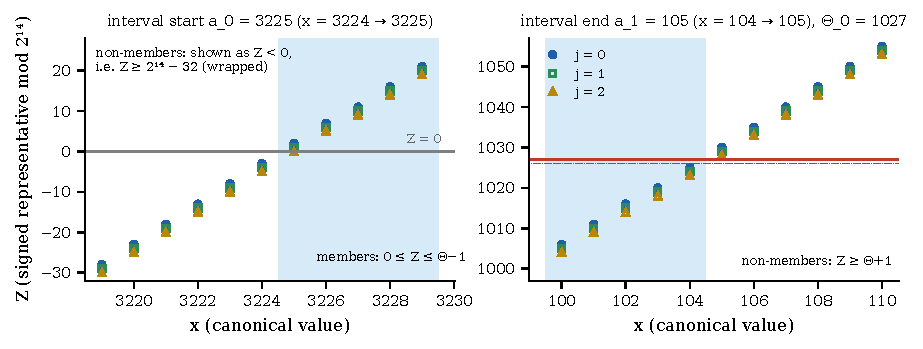
\includegraphics[width=\textwidth]{figures/mathematics/fig_switch_boundaries.pdf}
\caption{$Z$ as a function of the canonical value $x$ near both ends of the wrapped interval $I_0$ ($d = 4$, $\Theta_0 = 1027$), for the three possible switching errors $j$. Members are shaded.
\emph{Left:} at the interval start, members begin at $Z \in [0, 2]$, and non-members just below $a_0$ wrap to $Z \ge 2^{14} - 32$, drawn as negative values.
\emph{Right:} at the interval end, the last member reaches at most $\Theta_0 - 1$ (dotted) and the first non-member at least $\Theta_0 + 1$.
Generated from \file{models/pams.py} by \file{paper/scripts/generate\_figures.py}.}\label{fig:boundaries}
\end{figure*}

\paragraph{H.~From equations to hardware.} \Cref{tab:map} names the RTL signals that compute each quantity. It also gives the pipeline stage at which each value is held, where stage $s$ means $s$ clock edges after the coefficient enters. A full cross-layer map, including gate-level regions and figure references, is in \cref{app:traceability} and \file{paper/CROSS\_LAYER\_TRACEABILITY.md}.

\begin{table*}[t]\centering\small
\caption{Mathematical quantities and the \sig{pams\_jqr} RTL that computes them (stage = register boundary at which the value is held).}\label{tab:map}
\setlength{\tabcolsep}{4pt}
\begin{tabularx}{\textwidth}{@{}p{3.4cm}Xp{6.4cm}@{}}
\toprule
quantity & hardware representation & RTL (stage) \\
\midrule
$x_i$ & 12-bit input, then two register stages & \sig{x$i$}, \sig{x$i$q} (1), \sig{x$i$r} (2) \\
$F_{14}(x_i)$ & $(x_i \cdot M) \gg 21$; two registered partial products, then sum & \sig{mh$i$}, \sig{ml$i$} (3), \sig{s$i$p} (4) \\
$e$, $\mathrm{qq}(r_c)$, $\mathrm{qq}(r_{c+1})$ & public logic from $(c, d)$ & \sig{e0r}, \sig{qcr}, \sig{qnr} (2) \\
$\Low_c$, $\Theta_c$ & \cref{eq:low,eq:thetaclosed} & \sig{lowrq}, \sig{thrq} (3), \sig{lowp} (4), \sig{th2} (5) \\
$\hat y_0, y_1, y_2$ & 14-bit operands, one per domain & \sig{y0}, \sig{y1}, \sig{y2} (5) \\
$Z$, $[Z < \Theta_c]$ & CSA + ripple carry + comparator: 38 HPC2, share-local XOR, delay registers & \sig{ug111}\ldots\sig{ug1542}, \sig{r105}\ldots (5--31) \\
$b$ (3 shares) & Boolean sharing & \sig{cdec}, \sig{cvalid} (31) \\
$D$ (3 shares) & AND accumulator over the ciphertext & \sig{uacc}, \sig{ufin}, \sig{dec}, \sig{dvalid} (35) \\
\bottomrule
\end{tabularx}
\end{table*}

\subsection{Verilog Implementation}\label{sec:rtl}
The final RTL is generated by \file{competitors/models/cgen.py} from the same building blocks as the frozen generator \file{models/gen.py}. With all optimizations disabled, the generator reproduces the frozen \file{rtl/pams.v} byte for byte. \file{final/rtl/pams\_jqr.v} has 2,747 lines.
\begin{itemize}
  \item Lines 1--19: the HPC2 module.
  \item Lines 21--56: the lane interface, input registers, public window logic and share-wise front end.
  \item Lines 58--1499: generated wire and register declarations.
  \item Lines 1500--1537: the 38 kernel gadget instances.
  \item Lines 1538--2729: share-local delay registers.
  \item Lines 2730--2746: the control pipeline and the accumulator.
\end{itemize}
All excerpts below are verbatim, with their source line numbers. \Cref{app:verilog} explains the remaining code.

\paragraph{Interface and input registers (lines 21--26).}\leavevmode\par
\lstinputlisting[firstline=21,lastline=26,firstnumber=21]{\RTL}
\begin{itemize}
  \item \textbf{Ports.} The three 12-bit shares arrive on \sig{x0..x2}, the public \sig{c} and \sig{mode} beside them, and \sig{vin}/\sig{first}/\sig{last} frame a ciphertext. The 120-bit port \sig{rnd} carries the fresh randomness of the cycle: 3 bits for each of the 40 gadgets.
  \item \textbf{Stage 1.} All inputs are registered; \sig{mode} is decoded to $d$ in \sig{d0}.
  \item \textbf{Domains.} The share index is kept in the signal names (\sig{x0q}, \sig{x1q}, \sig{x2q}), which is how the structural checks of \cref{sec:security} identify domains. Nothing ever combines two of these signals outside a gadget.
\end{itemize}

\paragraph{Public anchor and threshold (lines 31--45).}\leavevmode\par
\lstinputlisting[firstline=31,lastline=45,firstnumber=31]{\RTL}
\begin{itemize}
  \item \textbf{Closed forms.} This is \cref{eq:low,eq:thetaclosed}. \sig{qq} implements $\lfloor r\,2^{e}/q \rfloor$ with four constant comparisons (line~34), \sig{pr} is $(1 - 2c)\,q \bmod 2^{12}$ (line~38), and \sig{rmask} reduces it mod $2^{d+1}$.
  \item \textbf{Retiming (r).} The intermediate results \sig{qc}, \sig{qn}, \sig{e0} and \sig{c0} are registered at stage~2 (line~43). The remaining arithmetic producing \sig{lowr} = $\Low_c$ and \sig{thr} = $\Theta_c$ completes in the next stage (lines~44--45). This splits a public critical path (\cref{sec:circuit}) without adding latency.
  \item \textbf{Security.} Everything here is a function of public $(c, d)$ only.
\end{itemize}

\paragraph{Share-wise modulus switch (lines 47--56).}\leavevmode\par
\lstinputlisting[firstline=47,lastline=56,firstnumber=47]{\RTL}
\begin{itemize}
  \item \textbf{Partial products (stage 3, line~49).} Each share is split as $x_i = 2^6 x_{i,11:6} + x_{i,5:0}$, and both halves are multiplied by $M$ and registered. Line~49 is long because the generator emits all six products on one line.
  \item \textbf{Recombination (lines~50--51).} \sig{m$i$} recombines the halves, and \sig{s$i$} drops 21 bits to give $y_i = F_{14}(x_i)$ (\cref{eq:yi}), registered as \sig{s$i$p} at stage 4.
  \item \textbf{Anchoring (stage 5, line~56).} Share 0 receives $-\Low_c + 2$ (\cref{eq:y0}). Shares 1 and 2 pass unchanged. The public threshold is delayed alongside the data into \sig{th2}.
  \item \textbf{Locality.} Each multiplier sees one share only. The 14-bit outputs \sig{y0..y2} are the only secret inputs of the masked kernel.
\end{itemize}

\paragraph{Masked kernel: gadget instances and delay registers.}
The kernel is generated as flat wires, registers and \sig{hpc2} instances. Its first three gadgets implement bit 1 of the adder and comparator:
\lstinputlisting[firstline=1500,lastline=1502,firstnumber=1500]{\RTL}
\begin{itemize}
  \item \textbf{\sig{ug111}: CSA majority of bit 0, $T_1 = \mathrm{maj}(y_{0,0}, y_{1,0}, y_{2,0})$.} It uses $\mathrm{maj}(a, b, c) = ((a \oplus b) \wedge (a \oplus c)) \oplus a$. Its operand sharings $(y_{0,0}, y_{1,0}, 0)$ and $(y_{0,0}, 0, y_{2,0})$ are formed from the three single-domain bits without any XOR gate, because the third share is the constant 0.
  \item \textbf{\sig{ug134}: carry $c_2 = S_1 \wedge T_1$.} Here $S_1$ is held as three single-domain registered bits \sig{r106}, \sig{r108}, \sig{r110}.
  \item \textbf{\sig{ug128}: comparator step for bit 1.} It computes $\lt_2 = ((z_1 \oplus \bar\theta_1) \wedge (\lt_1 \oplus \theta_1)) \oplus \theta_1$, with $z_1 = S_1 \oplus T_1$ and the public $\theta_1$ applied to share 0.
  \item \textbf{Randomness.} Each instance takes its own 3-bit slice of \sig{rnd}.
\end{itemize}

The delay registers that align operands are plain share-local shift registers, for example
\lstinputlisting[firstline=1538,lastline=1548,firstnumber=1538]{\RTL}
Bit $k$ of each operand waits until the carry for bit $k$ arrives, about $2k$ cycles later. Each chain holds one share bit, so the registers never mix domains.

\paragraph{Control and accumulation (lines 2730--2746).}\leavevmode\par
\lstinputlisting[firstline=2730,lastline=2746,firstnumber=2730]{\RTL}
\begin{itemize}
  \item \textbf{Control.} \sig{vp}, \sig{fp} and \sig{lp} delay the public frame signals to stage 31, where \sig{cdec} (the output of \sig{ug1542}) is the per-coefficient decision.
  \item \textbf{Accumulator.} \sig{uacc} ANDs each decision into a running product. Its 2-cycle latency yields two interleaved chains (even and odd coefficients), which \sig{init\_p} starts at the first two coefficients of a ciphertext. \sig{ufin} ANDs the two chains into \sig{dec}, valid with \sig{dvalid} four cycles after the last coefficient's decision.
  \item \textbf{Throughput.} A new coefficient can enter every cycle (initiation interval 1). The ciphertext decision appears 35 cycles after its last coefficient entered, against 37 cycles for the baseline \sig{base\_jq}.
\end{itemize}

\subsection{Circuit Architecture and Physical Realization}\label{sec:circuit}

\begin{figure*}[t]\centering
\resizebox{\textwidth}{!}{% PAMS datapath (pams_jqr). Conceptual diagram reconstructed by hand from final/rtl/pams_jqr.v (signal names, widths
% and stages from the source; see FIGURE_PROVENANCE.md). Not an automatically extracted circuit.
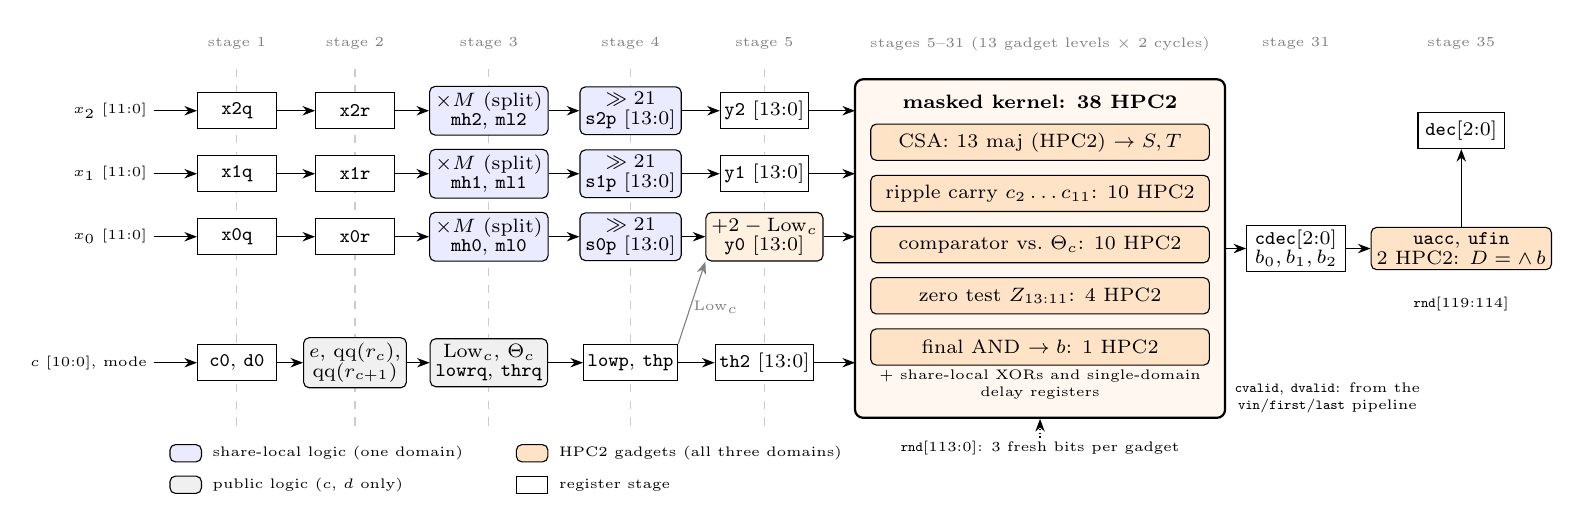
\begin{tikzpicture}[x=1cm,y=1cm,font=\scriptsize,>={Stealth[length=1.6mm]},
  reg/.style={draw,fill=white,minimum width=1.0cm,minimum height=0.46cm,inner sep=1.5pt,align=center},
  op/.style={draw,rounded corners=2pt,fill=#1,minimum height=0.46cm,inner sep=2pt,align=center},
  op/.default=blue!8,
  lab/.style={font=\tiny,inner sep=1pt}]
  % stage guides
  \foreach \s/\x in {1/1.55,2/3.05,3/4.75,4/6.55,5/8.25} {
    \draw[gray!40,dashed] (\x,-3.4) -- (\x,1.2);
    \node[gray,font=\tiny] at (\x,1.45) {stage \s};
  }
  \node[gray,font=\tiny] at (11.75,1.45) {stages 5--31 (13 gadget levels $\times$ 2 cycles)};
  \node[gray,font=\tiny] at (15.0,1.45) {stage 31};
  \node[gray,font=\tiny] at (17.1,1.45) {stage 35};
  % share lanes; share 0 is drawn next to the public lane so that the Low_c arrow crosses no other lane
  \foreach \i/\y in {2/0.6,1/-0.2,0/-1.0} {
    \node[lab,anchor=east] at (0.45,\y) {$x_{\i}$ [11:0]};
    \node[reg] (q\i) at (1.55,\y) {\sig{x\i q}};
    \node[reg] (r\i) at (3.05,\y) {\sig{x\i r}};
    \node[op] (m\i) at (4.75,\y) {$\times M$ (split)\\[-1pt]\sig{mh\i}, \sig{ml\i}};
    \node[op] (s\i) at (6.55,\y) {$\gg 21$\\[-1pt]\sig{s\i p} [13:0]};
    \draw[->] (0.5,\y) -- (q\i); \draw[->] (q\i) -- (r\i); \draw[->] (r\i) -- (m\i); \draw[->] (m\i) -- (s\i);
  }
  \node[op=orange!12] (y0) at (8.25,-1.0) {$+2-\mathrm{Low}_c$\\[-1pt]\sig{y0} [13:0]};
  \node[reg] (y1) at (8.25,-0.2) {\sig{y1} [13:0]};
  \node[reg] (y2) at (8.25,0.6) {\sig{y2} [13:0]};
  \draw[->] (s0) -- (y0); \draw[->] (s1) -- (y1); \draw[->] (s2) -- (y2);
  % public lane
  \node[lab,anchor=east] at (0.45,-2.6) {$c$ [10:0], mode};
  \node[reg] (c0) at (1.55,-2.6) {\sig{c0}, \sig{d0}};
  \node[op=gray!12] (pw) at (3.05,-2.6) {$e$, $\mathrm{qq}(r_c)$,\\[-1pt]$\mathrm{qq}(r_{c+1})$};
  \node[op=gray!12] (lo) at (4.75,-2.6) {$\mathrm{Low}_c$, $\Theta_c$\\[-1pt]\sig{lowrq}, \sig{thrq}};
  \node[reg] (lp) at (6.55,-2.6) {\sig{lowp}, \sig{thp}};
  \node[reg] (th) at (8.25,-2.6) {\sig{th2} [13:0]};
  \draw[->] (0.5,-2.6) -- (c0); \draw[->] (c0) -- (pw); \draw[->] (pw) -- (lo); \draw[->] (lo) -- (lp); \draw[->] (lp) -- (th);
  \draw[->,gray] (lp.north east) -- node[lab,pos=0.45,right] {$\mathrm{Low}_c$} (y0.south west);
  % masked kernel
  \node[draw,thick,fill=orange!6,rounded corners=3pt,minimum width=4.7cm,minimum height=4.3cm] (k) at (11.75,-1.15) {};
  \node[font=\scriptsize\bfseries] at (11.75,0.72) {masked kernel: 38 HPC2};
  \foreach \t/\y in {{CSA: 13 maj (HPC2) $\to S, T$}/0.2, {ripple carry $c_2 \ldots c_{11}$: 10 HPC2}/-0.45,
                    {comparator vs.\ $\Theta_c$: 10 HPC2}/-1.1,
                    {zero test $Z_{13:11}$: 4 HPC2}/-1.75, {final AND $\to b$: 1 HPC2}/-2.4}
    \node[op=orange!22,minimum width=4.3cm] at (11.75,\y) {\t};
  \node[lab,align=center] at (11.75,-2.88) {+ share-local XORs and single-domain\\ delay registers};
  \draw[->] (y2.east) -- (9.4,0.6); \draw[->] (y1.east) -- (9.4,-0.2); \draw[->] (y0.east) -- (9.4,-1.0);
  \draw[->] (th.east) -- (9.4,-2.6);
  \node[lab,anchor=north] (rnd) at (11.75,-3.55) {\sig{rnd}[113:0]: 3 fresh bits per gadget};
  \draw[->,densely dotted] (rnd.north) -- (k.south);
  % output and accumulator
  \node[reg,minimum width=1.25cm] (cdec) at (15.0,-1.15) {\sig{cdec}[2:0]\\[-1pt]$b_0, b_1, b_2$};
  \draw[->] (k.east) -- (cdec);
  \node[op=orange!22,minimum width=2.0cm] (acc) at (17.1,-1.15) {\sig{uacc}, \sig{ufin}\\[-1pt]2 HPC2: $D = \wedge\, b$};
  \draw[->] (cdec) -- (acc);
  \node[lab] at (17.1,-1.85) {\sig{rnd}[119:114]};
  \node[reg,minimum width=1.1cm] (dec) at (17.1,0.35) {\sig{dec}[2:0]};
  \draw[->] (acc) -- (dec);
  \node[lab,align=center] at (15.4,-3.05) {\sig{cvalid}, \sig{dvalid}: from the\\ \sig{vin}/\sig{first}/\sig{last} pipeline};
  % legend
  \node[op,minimum height=0.22cm,minimum width=0.4cm] at (0.9,-3.75) {}; \node[lab,anchor=west] at (1.2,-3.75) {share-local logic (one domain)};
  \node[op=gray!12,minimum height=0.22cm,minimum width=0.4cm] at (0.9,-4.15) {}; \node[lab,anchor=west] at (1.2,-4.15) {public logic ($c$, $d$ only)};
  \node[op=orange!22,minimum height=0.22cm,minimum width=0.4cm] at (5.3,-3.75) {}; \node[lab,anchor=west] at (5.6,-3.75) {HPC2 gadgets (all three domains)};
  \node[reg,minimum height=0.22cm,minimum width=0.4cm] at (5.3,-4.15) {}; \node[lab,anchor=west] at (5.6,-4.15) {register stage};
\end{tikzpicture}
}
\caption{\PAMS{} datapath (\sig{pams\_jqr}). This is a conceptual diagram reconstructed from the RTL; widths and stage numbers are those of the source.
\textbf{Share lanes (blue):} each share is processed only within its own domain.
\textbf{Public lane (grey):} depends only on $(c, d)$.
\textbf{Masked kernel (orange):} the only place where domains meet, and only inside the 38 HPC2 gadgets. Each gadget takes 3 fresh bits from \sig{rnd}.
\textbf{Accumulator:} two further gadgets combine the per-coefficient decisions of a ciphertext.
Stage $s$ = number of clock edges after the coefficient enters.}\label{fig:datapath}
\end{figure*}

\paragraph{Architectural level.}
\Cref{fig:datapath} shows the complete datapath, organized as five stages of share-local front end followed by the masked kernel.
\begin{itemize}
  \item \textbf{Front end.} Three identical share lanes run in parallel with the public lane that produces $\Low_c$ and $\Theta_c$. The two meet only at stage 5, where the public $-\Low_c + 2$ is added to share 0 and $\Theta_c$ enters the kernel as public data.
  \item \textbf{Kernel.} It consumes the three 14-bit operands. Thirteen HPC2 levels of two cycles each produce the three-share decision at stage 31.
  \item \textbf{Accumulator.} It produces the ciphertext decision at stage 35.
\end{itemize}

\paragraph{Gate level.}
Synthesis keeps every \sig{hpc2} instance as a separate module, so the gadget boundary survives in the mapped netlist.
\begin{itemize}
  \item \textbf{Inside the gadget.} \Cref{app:hpc2} shows the mapped gadget extracted from the synthesized netlist: 30 \sig{DFF\_X1}, 15 \sig{AND2\_X1}, 6 \sig{XOR2\_X1} and 12 \sig{XNOR2\_X1} cells, $180.35\um$.
  \item \textbf{Around the gadgets.} \Cref{fig:slice} is an automatically extracted subcircuit of the \emph{top-level} netlist around the three bit-1 gadgets above. It shows every mapped cell in the fan-in of their \sig{a}/\sig{b} pins, up to registers or three logic levels.
  \item \textbf{What the slice shows.} The registered single-domain operand bits (e.g.\ \sig{r106}, \sig{r108}, \sig{r110} $= S_1$) feed gadget ports directly, and the only gates between gadgets are two-input XOR/XNOR cells within one share domain.
  \item \textbf{Synthesis restructuring.} ABC realized the RTL XOR \sig{x115} as an \sig{XNOR2} that produces its complement (the cell labelled "ABC-internal net"), and absorbed the inversion into the \sig{XNOR2} that realizes \sig{x120}. Both cells stay on share 0. One-to-one RTL-to-gate correspondence therefore holds for registers and gadget boundaries, not for every combinational XOR.
\end{itemize}

\begin{figure*}[t]\centering
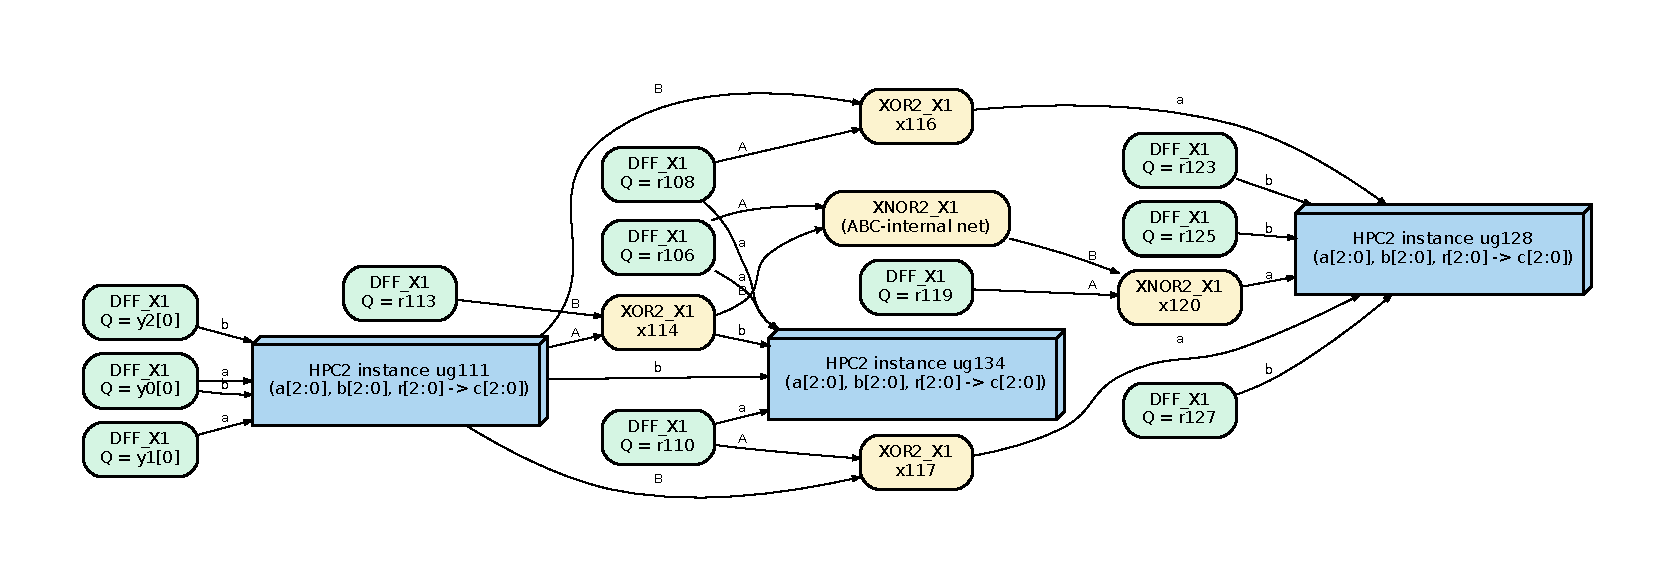
\includegraphics[width=0.9\textwidth]{figures/gates/slice_bit1.pdf}
\caption{Real mapped subcircuit around the bit-1 gadgets of \sig{pams\_jqr}, automatically extracted from \file{competitors/runs/syn\_pams\_jqr\_p0/mapped.json} (Yosys flow B, mapping 0) and drawn with Graphviz.
\textbf{Gadgets:} \sig{ug111} (CSA majority, bit 0), \sig{ug134} (carry $c_2$) and \sig{ug128} (comparator step $\lt_2$).
\textbf{Other cells:} green = \sig{DFF\_X1} (Q net named), yellow = combinational cells.
\textbf{Edges:} solid = into gadget port \sig{a} or cell input \sig{A}; dashed = into gadget port \sig{b} or cell input \sig{B}.}\label{fig:slice}
\end{figure*}

\paragraph{Physical level.}
\Cref{fig:placement} draws every placed standard cell of the routed reference runs (target 1.2\ns, seed 1, utilization 50\,\%), from OpenROAD's final DEF, at the same scale for both designs. Cells are classified by instance hierarchy and master cell.
\begin{itemize}
  \item \textbf{Gadgets (blue).} They occupy $7{,}242\um$ in \PAMS{} and $10{,}329\um$ in the baseline. This includes the hold buffers and tie cells OpenROAD inserted inside gadget hierarchies.
  \item \textbf{Pipeline and alignment flip-flops (green):} $5{,}851$ vs.\ $6{,}783\um$.
  \item \textbf{Other logic (orange):} mostly the share-wise multipliers, which cluster near the input pins; $3{,}906$ vs.\ $3{,}870\um$.
  \item \textbf{Buffers (grey):} $1{,}655$ vs.\ $2{,}199\um$.
  \item \textbf{Critical path (black).} The worst setup path of each design lies inside a share-wise multiplier stage: \sig{x1r[5]}$\to$\sig{ml1[23]} in \PAMS{} and \sig{x0r[9]}$\to$\sig{mh0[31]} in the baseline (\cref{fig:critpath}).
\end{itemize}
The OpenROAD-rendered routed layouts of the same runs are in \cref{app:physical}.

\begin{figure*}[t]\centering
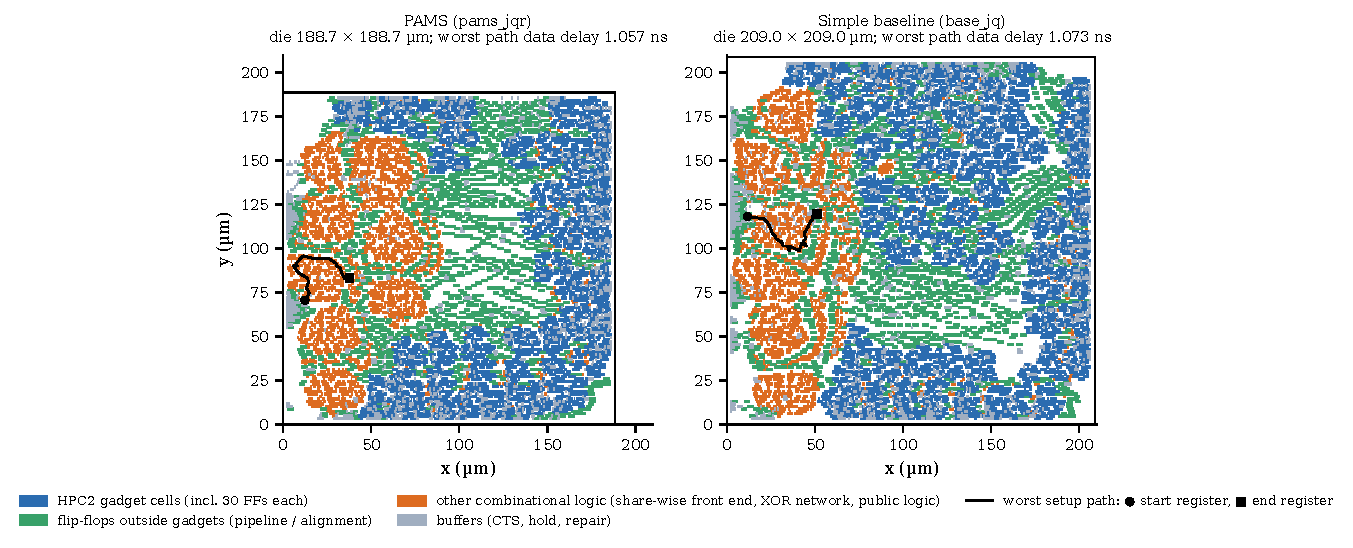
\includegraphics[width=\textwidth]{figures/physical/fig_placement.pdf}
\caption{Placed standard cells of the routed reference runs (target 1.2\ns, seed 1), drawn from the OpenROAD DEF files at equal scale. Tap and filler cells are omitted. The black polyline connects the cells of the worst setup path from \file{timing.rpt} (\cref{fig:critpath}). \PAMS{} fits in a $188.7 \times 188.7\,\si{\micro\meter}$ die; the baseline needs $209.0 \times 209.0\,\si{\micro\meter}$ at the same 50\,\% utilization.}\label{fig:placement}
\end{figure*}

\section{Security Analysis}\label{sec:security}

\subsection{Claim and model}
\paragraph{Claim.} We claim the following for \sig{pams\_jqr}, and identically for the baseline \sig{base\_jq}:
\begin{quote}\itshape
The lane is second-order secure in the glitch-robust probing model, i.e.\ against any two glitch-extended probes over any number of clock cycles, provided the \sig{rnd} input supplies fresh uniform independent bits every cycle and the input shares are a uniform canonical sharing.
\end{quote}

\paragraph{Leakage model.} Following the robust probing model~\cite{faust2018,cassiers2021hpc}:
\begin{itemize}
  \item a probe on a combinational wire reveals, for one cycle, every register output and primary input in that wire's combinational fan-in;
  \item a probe on a register reveals its value.
\end{itemize}

\paragraph{What we do not claim.}
\begin{itemize}
  \item security in the transition-robust model;
  \item security of any random-number generator;
  \item resistance to physical attacks beyond probing, such as couplings, horizontal or vertical attacks, and fault injection.
\end{itemize}
\Cref{sec:sec-limits} discusses these.

\subsection{Argument structure}
The argument has three steps. Each is supported by a different kind of evidence, summarized in \cref{tab:secevidence}.

\begin{table*}[t]\centering\small
\caption{Security evidence for the final circuits. "Final" = the publication netlists of \sig{pams\_jqr} and \sig{base\_jq}; "frozen" = the original \sig{pams}/\sig{base} designs evaluated in Phase XII.}\label{tab:secevidence}
\setlength{\tabcolsep}{4pt}
\begin{tabularx}{\textwidth}{@{}p{3.3cm}p{2.6cm}Xp{3.4cm}@{}}
\toprule
property & tool / method & result & applies to \\
\midrule
HPC2 gadget is glitch-robust 2-PINI & SILVER~\cite{knichel2020silver} (formal, BDD-based) & both mapped gadget variants (v0, v1): probing, NI, PINI and uniformity secure at order 2 in the standard and robust models; robust SNI only at order 1, as expected for a PINI-but-not-SNI gadget. Three broken variants (unregistered refresh, mask reuse, recombination) fail. & every gadget of all 24 final synthesis / P\&R-input netlists is byte-identical to v0 or v1 \\
gadget under transitions and pipelining & PROLEAD~\cite{mueller2022prolead} (statistical) & order 2, glitches + transitions, multivariate, four back-to-back executions, $2^{22}$ simulations: max $-\log_{10} p = 4.2$--$4.6$ over \num{6984} probing sets, no leakage; the three broken variants give $p \to 0$ & both gadget variants \\
preconditions of trivial PINI composition & \file{compcheck.py} (structural; with negative controls) & no net outside gadgets depends on two share domains; every random bit reaches exactly one gadget $r$-port; gadget input/output share $i$ is domain $i$; every routed gadget equals the verified gadget cell by cell & 5 synthesis mappings, P\&R inputs, and all 40 valid and DRC-failing routed runs of both finalists \\
constant time & cone analysis of \sig{cvalid}/\sig{dvalid} & timing outputs depend on no share and no random bit & 12 final netlists \\
whole-lane leakage & PROLEAD, robust glitches + transitions & no confirmed leakage; negative controls detected (\cref{tab:prolead}) & final \sig{pams\_jqr} (focused) and frozen \sig{pams}/\sig{base} (extensive) \\
\bottomrule
\end{tabularx}
\end{table*}

\paragraph{Step 1: the gadget.}
Every nonlinear operation is an instance of one HPC2 module, kept as a separate hierarchy level during synthesis. Synthesis maps this module in exactly two ways (variants v0 and v1) across all mappings and all designs.
\begin{itemize}
  \item \textbf{SILVER.} It verifies each variant exhaustively as glitch-robust 2-PINI.
  \item \textbf{PROLEAD.} It finds no leakage, even with transitions, when the gadget is executed every cycle.
  \item \textbf{Final netlists.} Every gadget instance in the final netlists is one of these two byte-identical variants (\file{final/runs/gadget\_identity.json}).
  \item \textbf{Routing.} P\&R adds buffers, resizes cells and ties constant shares inside gadget hierarchies. The G-check confirms that each routed gadget is still the verified gadget once those buffers are collapsed.
\end{itemize}

\paragraph{Step 2: composition.}
Outside the gadgets, the lane consists only of:
\begin{itemize}
  \item share-local operations: per-share multipliers, XORs of two values of the same domain, delay registers;
  \item public logic: the window constants and the control pipeline;
  \item operations that combine a public value with one share: $-\Low_c + 2$ on share 0, $\bar\theta_k$ on share 0.
\end{itemize}
\Cref{fig:domains} shows the resulting structure. Three domain columns interact only through HPC2 gadgets, each fed by its own fresh random bits. For such a circuit the trivial composition theorem of PINI~\cite{cassiers2020pini}, extended to glitches in the HPC framework~\cite{cassiers2021hpc}, implies that the lane is glitch-robust 2-PINI.

The theorem's preconditions are structural, and \file{compcheck.py} checks them mechanically on every netlist. The checker is our own code. It has negative controls: an exposed decision, a partial recombination and reused masks are all flagged.

\begin{figure}[t]\centering
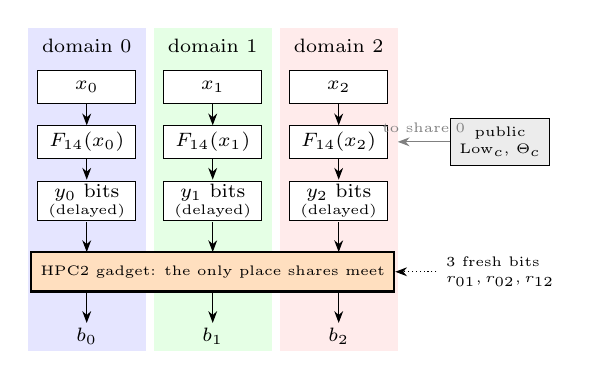
\begin{tikzpicture}[x=1cm,y=1cm,font=\scriptsize,>={Stealth[length=1.5mm]},
  bx/.style={draw,fill=white,align=center,minimum width=1.25cm,minimum height=0.42cm,inner sep=1pt}]
  \foreach \i/\x/\c in {0/0.8/blue!10,1/2.4/green!10,2/4.0/red!8} {
    \fill[\c] (\x-0.75,-3.35) rectangle (\x+0.75,0.75);
    \node at (\x,0.52) {domain \i};
    \node[bx] at (\x,0) {$x_{\i}$};
    \node[bx] at (\x,-0.7) {$F_{14}(x_{\i})$};
    \node[bx] at (\x,-1.45) {$y_{\i}$ bits\\[-2pt]{\tiny (delayed)}};
    \draw[->] (\x,-0.21) -- (\x,-0.49); \draw[->] (\x,-0.91) -- (\x,-1.18);
  }
  \node[draw,fill=gray!15,align=center,font=\tiny] (pub) at (6.05,-0.7) {public\\$\mathrm{Low}_c$, $\Theta_c$};
  \draw[->,gray] (pub.west) -- (4.75,-0.7) node[pos=0.5,above,font=\tiny] {to share 0};
  \node[draw,thick,fill=orange!25,minimum width=4.6cm,minimum height=0.5cm,font=\tiny] (g) at (2.4,-2.35) {HPC2 gadget: the only place shares meet};
  \foreach \x in {0.8,2.4,4.0} \draw[->] (\x,-1.72) -- (\x,-2.1);
  \foreach \x in {0.8,2.4,4.0} \draw[->] (\x,-2.6) -- (\x,-3.0);
  \node at (0.8,-3.17) {$b_0$}; \node at (2.4,-3.17) {$b_1$}; \node at (4.0,-3.17) {$b_2$};
  \node[align=left,font=\tiny] (rr) at (6.05,-2.35) {3 fresh bits\\ $r_{01}, r_{02}, r_{12}$};
  \draw[->,densely dotted] (rr.west) -- (g.east);
\end{tikzpicture}
\caption{Share-domain structure of \PAMS{} (conceptual). Every computation on secret data happens within one domain column, apart from HPC2 gadgets. Public values enter only share 0. Each gadget consumes three fresh random bits and returns one output share per domain.}\label{fig:domains}
\end{figure}

\paragraph{Step 3: what changed from the frozen design.}
The extensive Phase XII evaluation was done on the original \sig{pams}. The publication circuit \sig{pams\_jqr} differs from it in three ways:
\begin{itemize}
  \item single-domain operand bits are delayed instead of three-share sums;
  \item each share's multiplier has an extra register stage;
  \item the public window logic is retimed.
\end{itemize}
All three move registers within one domain or within public logic. None changes the gadget network, gadget inputs, gadget count or random-bit assignment. The composition argument therefore carries over unchanged, and its preconditions were re-checked on the final netlists. The \emph{statistical} whole-lane evidence for \sig{pams\_jqr}, however, is a focused campaign that is smaller than the frozen-design campaign (\cref{tab:prolead}). We do not claim that the two received identical testing.

\subsection{Statistical leakage detection with PROLEAD}\label{sec:prolead}
\paragraph{Configuration.} PROLEAD~\cite{mueller2022prolead} simulates the gate-level netlist and applies a fixed-versus-random G-test to the joint distribution of each probing set. We used:
\begin{itemize}
  \item the robust (glitch-extended) model with transitions enabled;
  \item one simulation = a 36-coefficient ciphertext streamed at one coefficient per cycle;
  \item a fixed group of boundary-adjacent coefficients that all match, against random coefficients;
  \item fresh \sig{rnd} every cycle.
\end{itemize}
A fixture turns the tested value into a uniform canonical 3-sharing; its signals are excluded from probing. A self-test with one deliberately wrong coefficient makes PROLEAD's output check fail, which confirms that the simulated end cycle is right.

\paragraph{Why flagged sets appear without leakage.} PROLEAD flags a probing set when $-\log_{10} p > 5$, a per-set threshold. A lane test evaluates $10^5$ to $10^6$ sets. Under the null hypothesis, the median of the \emph{maximum} $-\log_{10} p$ over $N$ independent sets is $-\log_{10}(1 - 2^{-1/N}) \approx \log_{10}(N/\ln 2)$, which is 5.0 for $N = \num{71568}$ and 5.85 for $N = \num{493055}$. Flags near those values are expected even for a leak-free circuit.

\paragraph{Confirming a flag.} We therefore re-test every flagged set alone with more simulations. A real leak grows roughly linearly in $-\log_{10} p$ with the number of simulations; a multiple-testing artefact decays toward the single-test null. PROLEAD~3.1.0 does not seed its random generator in hardware mode, so a rerun with the same simulation count replays the same data. Confirmations therefore always use a larger count, whose first part equals the screening data.

\begin{table}[t]\centering\small
\caption{Lane-level PROLEAD results (robust glitches + transitions). "null" = expected maximum under no leakage. Confirmations re-test the flagged set alone with $2^{22}$ (frozen base o1: $2^{24}$) simulations.}\label{tab:prolead}
\setlength{\tabcolsep}{2.5pt}
\resizebox{\columnwidth}{!}{%
\begin{tabular}{@{}llrrrr@{}}
\toprule
netlist & order, cycles & sims & max & null & confirm \\
\midrule
\sig{pams\_jqr} & 1, all 72 & $2^{20}$ & 5.53 & 5.01 & 0.78 \\
\sig{pams\_jqr} & 2, cycle 36 & $2^{18}$ & 5.21 & 5.85 & 0.44 \\
\sig{pams\_jqr} NC partial recomb. & 2, 36 & $2^{16}$ & \textbf{41.4} & 5.85 & -- \\
\midrule
frozen \sig{pams} & 1, all 70 & $2^{22}$ & 4.47 & 4.99 & -- \\
frozen \sig{pams} & 2, 34 & $2^{20}$ & 5.96 & 5.82 & 1.81 \\
frozen \sig{base} & 1, all 72 & $2^{22}$ & 5.46 & 5.14 & 1.59 \\
frozen \sig{base} & 2, 36 & $2^{20}$ & 6.79 & 6.11 & 1.20 \\
frozen NC (4 controls) & 1--2 & $\le 2^{18}$ & 22.5--$\infty$ & $\le 6.1$ & -- \\
\bottomrule
\end{tabular}}
\end{table}

\paragraph{Results.} \Cref{tab:prolead} summarizes the campaigns (details in \cref{app:prolead}).
\begin{itemize}
  \item \textbf{No confirmed leakage.} No probing set of any real design survives confirmation. Every flagged maximum decays to 0.4--1.8 when re-tested with more data.
  \item \textbf{Negative controls detected.} Each function-changing control is found with a large margin above the null: an exposed decision, a partial recombination $b_0 \oplus b_1$ on an output, and a reused mask inside one gadget. The partial recombination on \sig{pams\_jqr} reaches $-\log_{10} p = 41.4$ against a null of 5.85.
\end{itemize}

\paragraph{What this does and does not show.} The results show that, at the stated simulation counts and in the simulated leakage model, no first- or second-order leakage was detected, and that the test can detect injected flaws. They are not a proof:
\begin{itemize}
  \item absence of detection is bounded by the number of simulations;
  \item second order was evaluated at one steady-state cycle per lane;
  \item the simulated leakage model is not a physical device.
\end{itemize}

\subsection{Remaining limitations of the security argument}\label{sec:sec-limits}
\paragraph{Transitions.} Glitch-robust PINI composition does not imply transition robustness. Cassiers and Standaert's transition-robust composition theorem~\cite{cassiers2021trans} requires either O-PINI gadgets or PINI gadgets without adjacent executions. Neither holds here:
\begin{itemize}
  \item HPC2 is not O-PINI;
  \item every gadget executes every cycle;
  \item in the accumulator, execution $k$ feeds execution $k + 2$.
\end{itemize}
Our evidence for transitions is therefore only statistical. An O-PINI accumulator or idle cycles would make the theorem applicable. This is not implemented, and the same limitation applies to the baseline.

\paragraph{Randomness.} The lane consumes 120 fresh bits per cycle but does not generate them.
\begin{itemize}
  \item With a deterministic PRNG (e.g.\ unrolled Trivium~\cite{cassiers2024rng}), the guarantee becomes computational.
  \item The PRNG's own leakage lies outside this analysis.
  \item Separate generator instances must be seeded independently.
\end{itemize}

\paragraph{Physical attacks.} Probing security of the comparison does not prevent the vertical and template attacks of Hermelink et al.~\cite{hermelink2024}. It also does not prevent implementation-level leakage caused by parallelism, as Ranney et al.\ observed on FPGA~\cite{ranney2026}. We performed no measurements on hardware.

\paragraph{Integration.} The upstream sharing is assumed uniform and canonical. The decision shares must reach only masked consumers, and \sig{cdec} is a test output that must not be connected to unprotected logic.

\section{Experimental Methodology}\label{sec:method}

\subsection{Designs and the design contract}
Both designs implement one contract (\file{competitors/DESIGN\_CONTRACT.md}):
\begin{itemize}
  \item exact $[\Comp(x) = c]$ for all $x$, all $c$ and $d \in \{4,5,10,11\}$ selected per coefficient;
  \item three canonical arithmetic input shares mod $q$, and three-share Boolean outputs that are never recombined;
  \item one coefficient per cycle, sustained;
  \item the same HPC2 gadget, the same share-local style, the same accumulator and the same control pipeline;
  \item 3 fresh random bits per gadget per cycle, supplied externally.
\end{itemize}

\paragraph{The two finalists.}
\begin{itemize}
  \item \textbf{\sig{pams\_jqr}:} \PAMS{}.
  \item \textbf{\sig{base\_jq}:} the Simple method~\cite{fritzmann2022,danvers2023}, with $y_i = \lfloor x_i 2^{24}/q \rfloor \gg (11 - d)$. It subtracts $(2c - 1)\,2^{12} - 1$, a $t = 13$ fractional-bit offset found exhaustively to be the minimal exact one (\cref{app:baseline}), and tests the top $d$ bits of a 24-bit sum for zero. The test uses a carry-free top region and an early OR tree.
\end{itemize}

\paragraph{Generic optimizations, applied to both.}
\begin{itemize}
  \item \textbf{j:} delay single-domain operand bits instead of 3-share sums.
  \item \textbf{q:} two extra share-wise front-end pipeline stages, splitting the constant multiplier.
\end{itemize}

\paragraph{The PAMS-specific retiming r.}
\PAMS{} additionally receives \textbf{r}, which retimes its public window logic into the existing stages. The baseline has no equivalent need. In the baseline's synthesis STA its public offset logic needs at most $0.595\ns$ (arrival plus setup), while all of its share-wise stages need about $1.0\ns$: partial products $1.027$, sum $1.017$, shift and offset $0.995$. In \PAMS{} the public stage is critical ($1.033\ns$) and the share-wise stages need $0.99$--$1.02\ns$ (\file{final/runs/pubpaths\_*.txt}). After these optimizations both designs are balanced at the limit of a two-stage front end.

\paragraph{Why Simple is the baseline.}
The competitor study (\cref{app:competitors}) also built and synthesized lanes of four other kinds:
\begin{itemize}
  \item a Bos-style exact interval check (91 gadgets);
  \item HOCompress precision ($t = 14$, 59 gadgets);
  \item Brent--Kung (X2X-style) prefix carries (75 gadgets);
  \item a lower bound for Coron et al.'s arithmetic zero test, at least $33{,}500\um$ of unmasked multipliers alone.
\end{itemize}
All were dominated by Simple. The original, less optimized baseline of our first study is kept only as a historical reference.

\subsection{Synthesis and static timing}
\paragraph{Generation and synthesis.} RTL is generated deterministically by \file{competitors/models/cgen.py}. It is synthesized with:
\begin{itemize}
  \item Yosys 0.33~\cite{yosys}: \texttt{synth -flatten -noabc}, \texttt{dfflibmap};
  \item ABC~\cite{brayton2010abc} with BUF\_X1 drive, a 5\,fF load and delay target $-D\,500$;
  \item the Nangate45 typical library~\cite{nangate45}.
\end{itemize}
The \sig{hpc2} module is kept as a separate hierarchy level (\texttt{keep\_hierarchy}) so that gadget boundaries survive. Five mappings per design (ABC $-D$ 500 with 0, 3 or 6 extra pad modules, $-D$ 400, $-D$ 650) estimate mapping variability; medians are reported.

\paragraph{Static timing.} OpenSTA 3.1.0~\cite{opensta} analyses four data-path groups (in2reg, reg2reg, reg2out, in2out) with I/O at the clock edge, 0.05\ns{} input transition and 5\,fF output load. The reported delay is the minimum clock period including setup.

\paragraph{Why synthesis is not enough.} Synthesis area counts only cell area, and its timing ignores wires. After placement and routing, the following change area and delay:
\begin{itemize}
  \item clock-tree buffers, hold-fixing buffers, setup repair, tie cells and wire parasitics;
  \item for designs dominated by registers, as these are, especially clock and hold buffering.
\end{itemize}
Physical results are therefore the basis of our final comparison.

\subsection{Placement and routing}
\paragraph{Flow.} We use OpenROAD~\cite{ajayi2019openroad} from the OpenROAD-flow-scripts image 26Q3, with the Nangate45 platform. The flow script (\file{final/tools/pnr\_final.tcl}) is identical for both designs:
\begin{enumerate}
  \item floorplan at 50\,\% utilization (aspect 1, 2\,\si{\micro\meter} core margin), I/O placement and PDN;
  \item global placement at density 0.6, first wirelength-driven, then timing-driven;
  \item repair\_design, detailed placement;
  \item clock-tree synthesis (BUF\_X4/BUF\_X8);
  \item setup repair, and hold repair with a 60\,\% buffer cap;
  \item global routing (50 congestion iterations), setup repair, detailed routing (64 iterations);
  \item filler insertion, and RCX parasitic extraction for final STA.
\end{enumerate}
Inputs are flow-C netlists: flow B with the platform's don't-use cells removed.

\paragraph{Seeds.} We vary only the random seed of global placement and I/O placement. Seeds 1--7 were used for both designs at every target.
\begin{itemize}
  \item \textbf{Seeds give different layouts.} Between seeds 1 and 2 (and between 2 and 3), 84\,\% of the instances common to both runs move (mean displacement 11--12\,\si{\micro\meter}) and 170--171 of 181 I/O pins move (\file{final/models/placediff.py}).
  \item \textbf{A seed reproduces its layout.} Repeating seed 1 at 2.0\ns{} reproduces the earlier unseeded run bit for bit.
  \item \textbf{What the seeds sample.} The runs sample implementation variation of one netlist under one flow. They are not independent physical samples, and statistics are read in that sense.
\end{itemize}

\paragraph{Clock targets.} Earlier studies used a loose 2.0\ns{} target, which both designs beat by 40--45\,\%. We added two targets near their practical limits:
\begin{itemize}
  \item \textbf{1.2\ns:} both close timing with margin.
  \item \textbf{1.1\ns:} both achieve about $1.07\ns$.
\end{itemize}
The bound was 21 runs per design, with a 90-minute wall-clock limit per run enforced by a watchdog. A run counts as \emph{valid} only if the flow finishes with zero DRC violations, RCX parasitics and non-negative hold slack. Every run is reported, including invalid ones.

\subsection{Metrics}
\begin{itemize}
  \item \textbf{Synthesized area:} sum of the liberty areas of the mapped cells, including gadget internals.
  \item \textbf{Routed cell area:} OpenROAD \texttt{design\_area} after routing, including inserted buffers and tie cells.
  \item \textbf{Die area:} the floorplanned die at 50\,\% utilization. It scales with the synthesized area and is an estimate of footprint, not a packaged chip.
  \item \textbf{Achieved period:} the target minus the worst setup slack over all four path groups, on RCX parasitics, with propagated clocks.
  \item \textbf{Gadgets:} HPC2 instances in the RTL, equal in every netlist.
  \item \textbf{Randomness:} the width of \sig{rnd}, 3 bits per gadget per cycle.
  \item \textbf{Latency:} clock cycles from coefficient input to \sig{cvalid}, and from the last coefficient to \sig{dvalid}.
  \item \textbf{Statistics:} exact two-sided rank-sum tests over all $\binom{14}{7}$ label assignments; the smallest attainable $p$ for 7 against 7 runs is $0.0006$.
\end{itemize}
Power was not measured. All numbers are EDA estimates.

\subsection{Functional verification}
Every design was simulated with Icarus Verilog~\cite{icarus} at RTL, at gate level, and as a routed netlist with liberty functions inlined. The systematic stimulus covers:
\begin{itemize}
  \item every interval boundary of every $(c, d)$: $a_c - 1$, $a_c$, $a_{c+1} - 1$, $a_{c+1}$;
  \item every $x \in [0, q)$ for every $d$, against $c = \Comp(x)$ and against $c + 1$.
\end{itemize}
That is \num{39112} coefficients in \num{7096} ciphertexts, with shares that include zeros and $q - 1$. A random, accept-heavy stimulus adds \num{6001} coefficients and \num{1086} ciphertexts on the routed netlists. All designs showed 0 mismatches at every level (\cref{app:functional}).

\section{Results}\label{sec:results}
All figures in this section are generated by \file{paper/scripts/generate\_figures.py} from the frozen result files:
\begin{itemize}
  \item \file{final/runs/pnr\_stats.json}: 42 seeded P\&R runs;
  \item \file{competitors/runs/cbench.json}: synthesis;
  \item the run directories' \file{final.def} and \file{timing.rpt}.
\end{itemize}
\Cref{tab:headline} collects the headline numbers.

\begin{table*}[t]\centering\small
\caption{Headline comparison of the final circuits. Synthesis: median [min, max] of 5 mappings. Routed: median [min, max] over the 7 valid seeds at each target, utilization 50\,\%. Improvement = (baseline $-$ \PAMS{}) / baseline; positive favours \PAMS{}.}\label{tab:headline}
\setlength{\tabcolsep}{4pt}
\resizebox{\textwidth}{!}{%
\begin{tabular}{@{}lrrr@{}}
\toprule
metric & \PAMS{} (\sig{pams\_jqr}) & baseline (\sig{base\_jq}) & improvement \\
\midrule
HPC2 gadgets & 40 & 57 & 29.8\,\% \\
fresh random bits per cycle & 120 & 171 & 29.8\,\% \\
synthesized cell area (\si{\micro\meter\squared}) & \num{17022} [\num{17001}, \num{17022}] & \num{21097} [\num{21097}, \num{21097}] & 19.3\,\% \\
synthesized delay (\si{\nano\second}) & 1.033 [1.033, 1.041] & 1.057 [1.057, 1.057] & 2.3\,\% \\
routed cell area @ 2.0\ns{} (\si{\micro\meter\squared}) & \num{18734} [\num{18706}, \num{18771}] & \num{23285} [\num{23266}, \num{23309}] & 19.5\,\% \\
routed cell area @ 1.2\ns{} & \num{18750} [\num{18710}, \num{18778}] & \num{23304} [\num{23278}, \num{23338}] & 19.5\,\% \\
die area (\si{\micro\meter\squared}) & \num{35596} & \num{43694} & 18.5\,\% \\
achieved period @ 2.0\ns{} target (\si{\nano\second}) & 1.156 [1.146, 1.165] & 1.198 [1.142, 1.255] & 3.6\,\% (inconclusive, $p = 0.073$) \\
achieved period @ 1.2\ns{} target & 1.094 [1.091, 1.097] & 1.105 [1.102, 1.111] & 1.0\,\% ($p = 0.0006$) \\
achieved period @ 1.1\ns{} target & 1.068 [1.062, 1.070] (7/7 valid) & 1.066 (1/7 valid) & $-0.2$\,\% (single run) \\
area $\times$ delay @ 1.2\ns{} (\si{\micro\meter\squared\nano\second}) & \num{20532} & \num{25761} & 20.3\,\% \\
flip-flops (all, incl.\ 30 per gadget) & \num{2494} & \num{3210} & 22.3\,\% \\
buffers after routing @ 1.2\ns{} & \num{1558} & \num{2081} & 25.1\,\% \\
initiation interval & 1 & 1 & -- \\
latency to \sig{cvalid} / to \sig{dvalid} after last coefficient (cycles) & 31 / 35 & 33 / 37 & 2 cycles \\
\bottomrule
\end{tabular}}
\end{table*}

\subsection{Area}
\Cref{fig:area} compares synthesized and routed cell area.
\begin{itemize}
  \item \textbf{Consistent across targets.} \PAMS{} is \num{19.3}\,\% smaller after synthesis and \num{19.5}\,\% smaller after routing at every target.
  \item \textbf{No overlap.} Every \PAMS{} run is smaller than every baseline run (rank-sum $p = 0.0006$, the minimum attainable).
  \item \textbf{Tiny spread.} Across seeds, cell area varies by at most 0.4\,\% in either design, so the 4,550\um{} gap is about 70 times the seed range.
  \item \textbf{Routing overhead.} Routing adds about \num{1700}\um{} to \PAMS{} and \num{2200}\um{} to the baseline, mostly clock and hold buffers.
  \item \textbf{Die (\cref{fig:die}).} At equal utilization the die shrinks from $209.0^2$ to $188.7^2\,\si{\micro\meter\squared}$, a reduction of \num{18.5}\,\%.
\end{itemize}

\begin{figure}[t]\centering
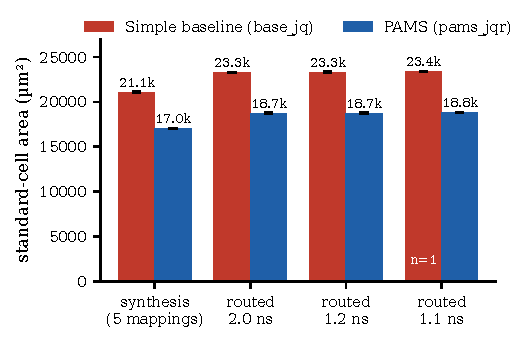
\includegraphics[width=\columnwidth]{figures/results/fig_area.pdf}
\caption{Standard-cell area: synthesis (median of 5 mappings) and routed cell area at three clock targets (median of valid seeds, error bars = min/max). At 1.1\ns{} only one baseline run is valid ($n = 1$).}\label{fig:area}
\end{figure}

\begin{figure}[t]\centering
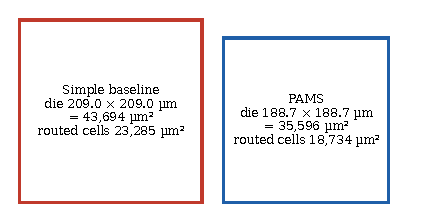
\includegraphics[width=\columnwidth]{figures/results/fig_die.pdf}
\caption{Estimated die footprint at 50\,\% utilization, drawn to scale (2.0\ns{} runs; the floorplan does not depend on the target).}\label{fig:die}
\end{figure}

\paragraph{Where the area goes.} \Cref{tab:resources} decomposes the synthesized area of mapping 0 by function (\file{paper/scripts/resources.py}; \cref{app:resources}). The 4,075\um{} difference comes from four sources:
\begin{itemize}
  \item 17 fewer gadgets: $17 \times 180.35 = 3{,}066\um$, three quarters of the saving;
  \item shorter delay chains: $-457\um$;
  \item the 14- instead of 24-bit share-wise operands without a mode shifter: $-1{,}286\um$ in front-end registers, logic and aligned operands;
  \item more public logic in \PAMS{}, which partly offsets the savings: $+873\um$ for $\Low_c$ and $\Theta_c$.
\end{itemize}

\begin{table}[t]\centering\small
\caption{Synthesized area by function (mapping 0, \si{\micro\meter\squared}). Combinational cells outside gadgets are attributed to the register group their fan-out reaches (approximate where ABC merged logic).}\label{tab:resources}
\setlength{\tabcolsep}{3pt}
\resizebox{\columnwidth}{!}{%
\begin{tabular}{@{}lrrr@{}}
\toprule
block & \PAMS{} & baseline & $\Delta$ \\
\midrule
HPC2 gadgets (40 / 57 $\times$ 180.35) & 7,214 & 10,280 & $-3{,}066$ \\
alignment (delay-chain) registers + logic & 3,558 & 4,016 & $-457$ \\
front-end registers ($x_r$, partial products, switched) & 1,081 & 1,411 & $-330$ \\
front-end logic (multipliers, sum, mode shift) & 2,610 & 3,033 & $-423$ \\
aligned operands $y_i$: registers + logic & 294 & 827 & $-533$ \\
public constant registers + logic & 1,337 & 464 & $+873$ \\
share-local XOR network at gadget inputs & 256 & 266 & $-10$ \\
input, control, accumulator, other & 672 & 801 & $-129$ \\
\midrule
total (equals reported synthesis area) & 17,022 & 21,097 & $-4{,}075$ \\
\bottomrule
\end{tabular}}
\end{table}

\subsection{Protected gadgets and randomness}
\Cref{fig:gadgets,fig:random} show the structural savings. The kernel needs 38 instead of 55 gadgets.
\begin{itemize}
  \item \textbf{CSA.} The narrower operands remove 10 of its gadgets.
  \item \textbf{Comparator.} The comparator against $\Theta_c$ on the low 11 bits plus the zero test of $Z_{13:11}$ (14 gadgets) replaces the baseline's carry-free zero test of its top 11 bits with an OR tree (20 gadgets). The ripple has two fewer carries.
  \item \textbf{Randomness.} Fresh randomness falls from 171 to 120 bits per cycle. At one coefficient per cycle, a generator must deliver \num{51} fewer bits every cycle. With 64-bit unrolled-Trivium instances~\cite{cassiers2024rng} that is two instances instead of three, but the generator is not included in any area figure.
\end{itemize}

\begin{figure}[t]\centering
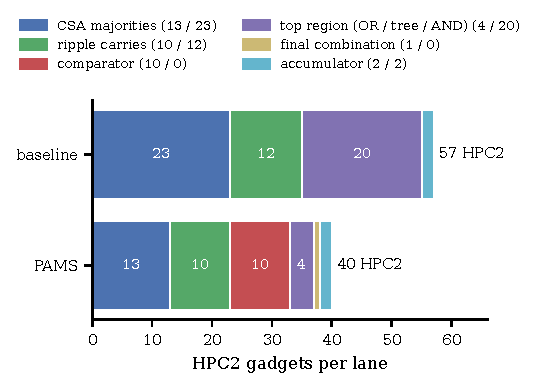
\includegraphics[width=\columnwidth]{figures/results/fig_gadgets.pdf}
\caption{HPC2 gadgets per lane by function (legend: \PAMS{} / baseline counts).}\label{fig:gadgets}
\end{figure}

\begin{figure}[t]\centering
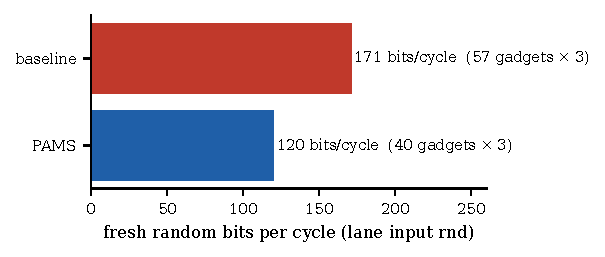
\includegraphics[width=\columnwidth]{figures/results/fig_random.pdf}
\caption{Fresh random bits consumed per cycle (3 per HPC2 gadget, second order).}\label{fig:random}
\end{figure}

\subsection{Timing}
\Cref{fig:timing} shows every run's achieved period.
\begin{itemize}
  \item \emph{2.0\ns{} target.} With no timing pressure, \PAMS{}'s median is 3.6\,\% lower. The baseline spreads widely across seeds (1.142--1.255\ns), and its fastest run beats PAMS's median. The distributions overlap ($p = 0.073$): \textbf{inconclusive}.
  \item \emph{1.2\ns{} target.} Timing-driven repair pulls both designs close to their limits, and the spread collapses to under 10\,ps. \PAMS{}'s period is lower in every seed ($p = 0.0006$), but only by 11\,ps (1.0\,\%). The seeds vary the layout of one netlist per design, so this separates the two layout distributions in this flow. It is not evidence of a general speed advantage (\cref{sec:method}).
  \item \emph{1.1\ns{} target.} \PAMS{} achieves 1.062--1.070\ns{} in all seven seeds. The only valid baseline run achieves 1.066\ns. Its five finished but DRC-failing runs reach 1.066--1.073\ns{}, so they show the same timing.
\end{itemize}
The two architectures have \textbf{comparable clock periods}. A difference of 1--4\,\% is not a timing advantage of practical size, and at the tightest target it disappears. \Cref{fig:adp} places every run in the area--delay plane: \PAMS{} occupies a lower band at every target, and its area-delay product is 19--23\,\% lower.

\begin{figure*}[t]\centering
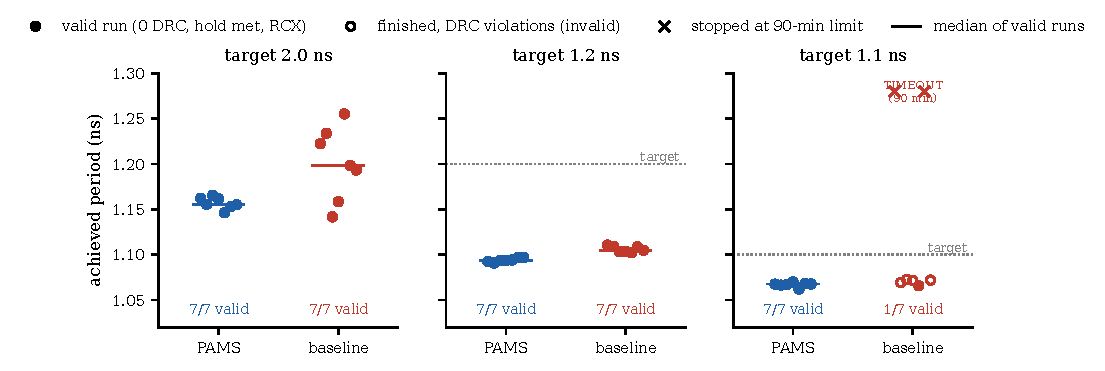
\includegraphics[width=\textwidth]{figures/results/fig_timing.pdf}
\caption{Achieved clock period of every P\&R run (seeds 1--7, offset horizontally by seed), at three targets. Filled = valid; hollow = finished with DRC violations; $\times$ = stopped at the 90-minute limit (no timing result).}\label{fig:timing}
\end{figure*}

\begin{figure}[t]\centering
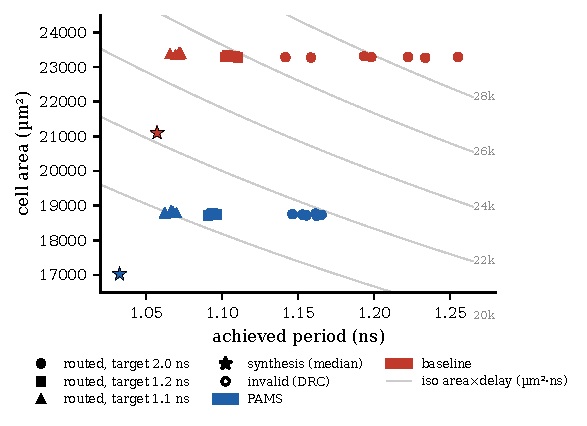
\includegraphics[width=\columnwidth]{figures/results/fig_adp.pdf}
\caption{Area versus achieved period for every routed run and for synthesis. Grey curves are iso-lines of area $\times$ delay.}\label{fig:adp}
\end{figure}

\paragraph{Why timing converges.} \Cref{fig:critpath} shows the worst routed paths at 1.2\ns.
\begin{itemize}
  \item \textbf{Both critical paths are in the share-wise front end.} \PAMS{} launches from \sig{x1r[5]} and captures at \sig{ml1[23]}: a partial product of the split constant multiplier, 1.057\ns{} of data path plus 0.179\ns{} of clock latency. The baseline's path, \sig{x0r[9]}$\to$\sig{mh0[31]}, has the same structure and a 1.073\ns{} data path.
  \item \textbf{Neither is in the masked kernel.} No gadget or comparator path is critical. Both front ends have been split until their stages balance near 1.0\ns{} (\cref{sec:method}).
  \item \textbf{The limit depends on the target.} Across all runs (\cref{tab:pnr-runs}), the limiting front-end stage changes:
  \begin{itemize}
    \item at 2.0\ns{}, \PAMS{} is limited by its public window logic (\sig{e0r}$\to$\sig{lowrq}), and the baseline by its mode-shift and offset stage (\sig{shp}$\to$\sig{y0}) or a partial product;
    \item at 1.2\ns{}, mostly by the partial products in both designs;
    \item at 1.1\ns{}, \PAMS{} by its public logic (\sig{c0r}$\to$\sig{lowrq}) and the baseline by its partial-product sum (\sig{mh}$\to$\sig{fq}).
  \end{itemize}
  \item \textbf{What remains.} The remaining difference is a few percent, between a 24-bit and a 34-bit constant multiplier stage and \PAMS{}'s public window stage. Further pipelining of either design, which for \PAMS{}'s public logic has no security cost, would reduce both periods toward a common limit set by the kernel. So we report no speed advantage.
\end{itemize}

\begin{figure*}[t]\centering
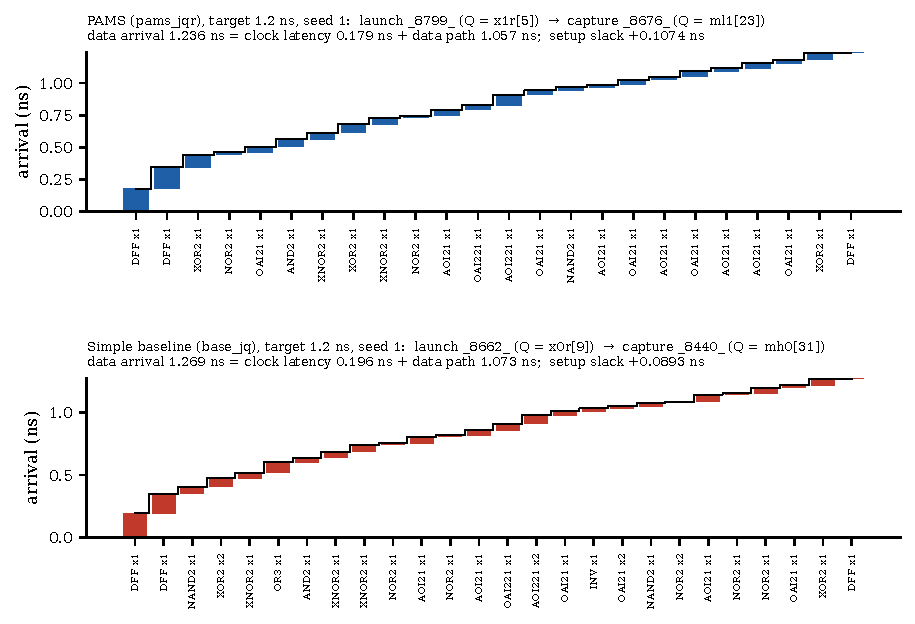
\includegraphics[width=\textwidth]{figures/physical/fig_critpath.pdf}
\caption{Worst setup paths of the routed reference runs (target 1.2\ns, seed 1), from OpenROAD \file{timing.rpt} on RCX parasitics. Bars = delay contributed by each cell (the first bar is the clock network latency at the launch flip-flop); black line = cumulative arrival. Both paths are a partial-product stage of the share-wise constant multiplier.}\label{fig:critpath}
\end{figure*}

\subsection{Physical realization and routability}
\Cref{fig:placement} (\cref{sec:circuit}) shows the placed designs at equal scale.
\begin{itemize}
  \item \textbf{Similar layouts.} In both designs the multipliers cluster near the input pins on the left, and the gadgets and delay chains fill the rest of the core.
  \item \textbf{Smaller PAMS core.} The \PAMS{} core is smaller in proportion to its cell area.
  \item \textbf{Less routing.} Total routed wirelength is \num{58067}--\num{58506}\,\si{\micro\meter} for \PAMS{} against \num{72529}--\num{73494}\,\si{\micro\meter} for the baseline at 1.1\ns, 20\,\% less.
\end{itemize}

At the 1.1\ns{} target this difference matters for routing (\cref{fig:routing}):
\begin{itemize}
  \item \textbf{PAMS:} every run routed DRC-clean in about 1.3 minutes.
  \item \textbf{Baseline:} only seed 5 did. Four runs finished with 1--6 residual DRC violations after 64 detailed-routing iterations (31--63 minutes), and two exceeded the 90-minute limit.
\end{itemize}

This is a flow-specific observation at one utilization: a lower utilization would probably let the baseline route, at a larger die. It shows that the smaller \PAMS{} netlist is easier to route under timing pressure in this flow, not that \PAMS{} is generally more routable. One valid baseline run is a single sample, not a distribution.

\begin{figure}[t]\centering
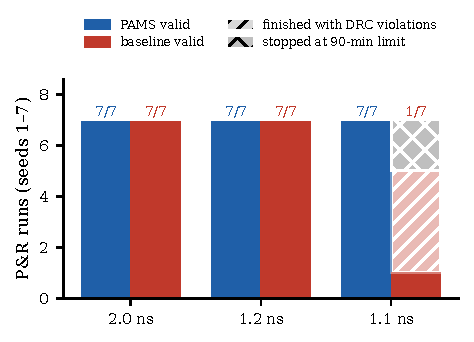
\includegraphics[width=\columnwidth]{figures/results/fig_routing.pdf}
\caption{Routing outcome of the seven seeds per design and target. At 1.1\ns, the baseline finished DRC-clean once, finished with DRC violations four times and was stopped twice.}\label{fig:routing}
\end{figure}

\subsection{Comparison with the original baseline}
Our first study compared the original, unpipelined designs. It reported \num{21.3}\,\% less area and \num{10.4}\,\% lower routed clock period against that original baseline. The area figure largely survives against the optimized baseline. The delay figure does not: it came from the original baseline's unpipelined 34-bit multiplier, and it vanishes once both designs are pipelined equally. We report it only as a historical comparison against a weaker baseline.

\section{Limitations}\label{sec:limits}
Each limitation below states its consequence for the claims of this paper.

\paragraph{Component-level evaluation.} \PAMS{} is a ciphertext-verification lane, not a full ML-KEM accelerator.
\begin{itemize}
  \item \textbf{Effect on scope.} The 19.5\,\% area reduction applies to this subsystem. In a complete masked decapsulation core, where NTT, sampling, hashing and the remaining conversions dominate, the relative saving is diluted by a factor we did not measure.
  \item \textbf{Effect on integration cost.} Integration questions are open: how the upstream re-encryption delivers canonical shares at one coefficient per cycle, and how \sig{dec} drives a masked implicit-rejection selection.
\end{itemize}

\paragraph{One library, one flow, no silicon, no power.} All numbers are Yosys/ABC, OpenSTA and OpenROAD estimates in the Nangate45 typical corner.
\begin{itemize}
  \item \textbf{Not measured:} other technologies, multi-corner analysis, clock uncertainty and on-chip-variation derating, and fabricated chips.
  \item \textbf{Power:} not reported. A vectorless estimate exists in the run directories but is not an energy measurement. Lower gadget and register counts make lower dynamic power plausible but unproven.
\end{itemize}

\paragraph{Randomness generation excluded.} The area figures exclude the random-number generator. The saving of 51 random bits per cycle reduces generator cost, for example from three to two unrolled-Trivium instances~\cite{cassiers2024rng}, but this was modelled in our earlier study, not implemented in the final comparison.

\paragraph{Canonical input shares.} Both designs require $0 \le x_i < 3329$ and do not check it. If the upstream logic produced 12-bit shares outside that range, correctness (not masking) could fail. The constant multiplier is inexact at $x_i = 3329$ and $4005$, and non-canonical inputs were not analysed completely (\cref{sec:exact}). The requirement must be met and documented at integration.

\paragraph{Finite physical-design sampling.} Seven seeds at each of three targets, at one utilization, sample implementation variation of one netlist per design.
\begin{itemize}
  \item \textbf{Area:} the conclusion is insensitive to this, given complete separation at every target.
  \item \textbf{Timing:} differences of 1--4\,\% lie within or near the seed spread. They depend on the target, and at the tightest target they vanish.
  \item \textbf{Routing:} the 1.1\ns{} routing result (7/7 against 1/7) may not hold at lower utilization or with other router settings.
\end{itemize}

\paragraph{Pipeline latency.} Both designs were pipelined with two extra share-wise stages. Their decision latency is 35 (\PAMS{}) and 37 (baseline) cycles after the last coefficient, at one coefficient per cycle. For a full ML-KEM-1024 ciphertext of 1,280 coefficients, verification takes about 1,315 cycles in total; the 2-cycle difference is negligible. Deeper pipelining would trade further registers for shorter clock periods in both designs and was not explored.

\paragraph{Security model.}
\begin{itemize}
  \item \textbf{Glitch-robust probing.} The supported claim is conditional: glitch-robust second-order probing security with ideal randomness and canonical uniform input sharings. It rests on SILVER (formal, gadget only), the published PINI theorem, and our structural checker. The checker is unreviewed project code, and no tool verified the whole lane formally.
  \item \textbf{Transitions.} Transition robustness is unproven: no applicable composition theorem exists for adjacent HPC2 executions.
  \item \textbf{Physical leakage.} Physical leakage was not measured, and attacks on the comparison function itself apply to any masked comparator~\cite{hermelink2024}.
  \item \textbf{Statistical evidence.} The PROLEAD evidence for the final circuit comes from a focused campaign, smaller than the campaign on the original design.
\end{itemize}

\paragraph{Architectural, not mathematical, novelty.} Every mathematical component of \PAMS{} is published~\cite{coron2023dil,coron2023poly,bos2021masking,azouaoui2023}, and exactness follows from the published lemma in a few lines. The contribution is the datapath that combines them into a single fixed-width comparator independent of $d$, and its measured consequence for area and randomness.

\paragraph{Limited access to two concurrent 2026 works.} Two hardware papers published in 2026 also mask an ML-KEM decapsulation core, and we could not obtain their full text. From their abstracts and associated artifacts:
\begin{itemize}
  \item Buschkowski et al.~\cite{buschkowski2026} automate mixed-domain masking and report an arbitrary-order masked ML-KEM decapsulation core; their abstract states that the final step "requires the re-encrypted data to be compressed before comparison" but does not specify the masked comparison method itself.
  \item Dobias et al.~\cite{dobias2026}, in \emph{PeerJ Computer Science}, present a first-order unified ML-DSA/ML-KEM core; the public artifact listing names a dataset file \texttt{sec\_decompressed\_comparison}, suggestive of a comparison performed after decompression rather than, as in \PAMS{}, on the compressed value directly, but we could not confirm this from the published text.
\end{itemize}
Neither paper's publicly accessible text specifies a fixed-width, pre-aligned masked comparator like \PAMS{}. Our literature, patent and code search covered the venues and preprint servers we judged most relevant, but was not exhaustive.

\section{Conclusion}\label{sec:conclusion}
\PAMS{} verifies masked ML-KEM ciphertext coefficients exactly. It switches every arithmetic share to one fixed 14-bit representation, anchors it at the public interval start of the received coefficient, and compares the masked sum with a per-coefficient public threshold.

Its ingredients are published: integer-error modulus switching, the $\lceil\log_2(nq)\rceil$ precision rule, interval anchoring and public-threshold comparison. Their combination makes the protected datapath independent of the compression width $d$.

Built as a three-share HPC2 lane at one coefficient per cycle, and compared with the strongest conventional exact lane we could construct under the same gadget, flow and generic optimizations, \PAMS{} achieves the following:
\begin{itemize}
  \item 29.8\,\% fewer secure gadgets (40 vs.\ 57);
  \item 29.8\,\% fewer fresh random bits per cycle (120 vs.\ 171);
  \item 19.5\,\% less routed standard-cell area for the lane;
  \item 18.5\,\% less estimated die area, consistently across seeds and clock targets;
  \item comparable clock periods, without a demonstrated general speed advantage.
\end{itemize}

Its glitch-robust second-order probing security is a conditional result. It assumes ideal randomness and canonical uniform input sharings. It rests on SILVER-verified gadgets, the published PINI composition theorem, and preconditions checked by our own structural checker. PROLEAD simulations detected no leakage that survived confirmation, which is statistical evidence only. Transition robustness, randomness generation and physical leakage remain open, as for the baseline.


\FloatBarrier
\bibliographystyle{plainnat}
\bibliography{references}

\clearpage
\onecolumn
\appendix
\section{Complete Mathematical Derivations}\label{app:math}
This appendix derives every formula used by \PAMS{} from the FIPS~203 definitions. It uses the notation of \cref{sec:math}: $q = 3329$, $n = 3$, $K = 14$, $F_K(v) = \lfloor 2^K v/q \rfloor$ for integers $v$, and canonical shares $x_i \in [0, q)$. The computational checks quoted were run on the frozen reference implementation (\file{models/pams.py}, \file{validation/math/}) and re-run for this paper where stated.

\subsection{Compression}\label{app:math-compress}
FIPS~203 defines $\Comp(x) = \lceil (2^d/q)\,x \rfloor \bmod 2^d$, where $\lceil y \rfloor$ is $y$ rounded to the nearest integer with ties rounded up, i.e.\ $\lceil y \rfloor = \lfloor y + \tfrac12 \rfloor$. Hence
\begin{equation}
  \Comp(x) = \Bigl\lfloor \frac{2^d x}{q} + \frac12 \Bigr\rfloor \bmod 2^d = \Bigl\lfloor \frac{2^{d+1} x + q}{2q} \Bigr\rfloor \bmod 2^d .
\end{equation}
A tie would require $2^{d+1}x + q \equiv 0 \pmod{2q}$. The left side is odd because $q$ is odd, while $2q$ is even, so ties never occur. The reference function \sig{compress} in \file{models/pams.py} implements exactly the integer form \texttt{((x << d) * 2 + Q) // (2 * Q) \% (1 << d)}.

\subsection{Compression intervals}\label{app:math-intervals}
Fix $d$ and $c \in [0, 2^d)$, and treat $x$ as an integer in $[0, q)$. Let $u = \lfloor (2^{d+1}x + q)/(2q) \rfloor \in [0, 2^d]$ be the value before the reduction mod $2^d$. Then $\Comp(x) = c$ iff $u = c$, or $u = 2^d$ and $c = 0$.
\begin{itemize}
  \item \emph{Case $u = c$.} We need $c \le (2^{d+1}x + q)/(2q) < c + 1$, i.e.\ $(2c - 1)q/2^{d+1} \le x < (2c + 1)q/2^{d+1}$. The upper bound is never an integer because $(2c+1)q$ is odd, so the integer solutions are
  \[ \Bigl\lceil \tfrac{(2c-1)q}{2^{d+1}} \Bigr\rceil \le x \le \Bigl\lceil \tfrac{(2c+1)q}{2^{d+1}} \Bigr\rceil - 1 . \]
  \item \emph{Case $u = 2^d$, $c = 0$.} We need $x \ge (2^{d+1} - 1)q/2^{d+1} = q - q/2^{d+1}$. These values are the integers in $[q - \lfloor q/2^{d+1} \rfloor, q)$.
\end{itemize}
For $c = 0$ the first case gives $0 \le x \le \lceil q/2^{d+1} \rceil - 1$ (the lower bound $\lceil -q/2^{d+1} \rceil$ is negative). Together with the second case this is the \emph{cyclic} interval that starts at $q - \lfloor q/2^{d+1} \rfloor = \lceil -q/2^{d+1} \rceil \bmod q$.

In all cases, therefore,
\begin{equation}\label{eq:app-interval}
  \Comp(x) = c \iff x \in [a_c, a_{c+1}) \text{ cyclically in } \Zq, \qquad a_c = \Bigl\lceil \frac{(2c-1)q}{2^{d+1}} \Bigr\rceil \bmod q ,
\end{equation}
with $a_{2^d} = a_0$. The reference model checks this closed form against the starts found by scanning $\Comp$, for all four $d$. \Cref{tab:widths} lists the resulting parameters.

\begin{table}[h]\centering\small
\caption{Per-width parameters (computed with \file{models/pams.py}). The interval for $c = 0$ wraps through $q-1 \to 0$ when $a_0 > a_1$.}\label{tab:widths}
\begin{tabular}{@{}rrrrrrrrr@{}}
\toprule
$d$ & $e = 13-d$ & $2^d$ values of $c$ & widths $|I_c|$ & $a_0$ & $a_1$ & $I_0$ wraps & $\Theta_c$ range & cases $(x,j,c)$ \\
\midrule
4 & 9 & 16 & 208, 209 & 3225 & 105 & yes & 1022--1027 & \num{159792} \\
5 & 8 & 32 & 104, 105 & 3277 & 53 & yes & 510--515 & \num{319584} \\
10 & 3 & 1024 & 3, 4 & 3328 & 2 & yes & 13--19 & \num{10226688} \\
11 & 2 & 2048 & 1, 2 & 0 & 1 & no & 3--9 & \num{20453376} \\
\bottomrule
\end{tabular}
\end{table}

\subsection{Share-wise modulus switching and the integer error}\label{app:math-lemma}
\paragraph{Floor remainders.} For any integer $v \ge 0$ write
\begin{equation}
  2^K v = q\,F_K(v) + \rho(v), \qquad \rho(v) = 2^K v \bmod q \in [0, q).
\end{equation}
Equivalently $F_K(v) = 2^K v/q - \varphi(v)$, where $\varphi(v) = \rho(v)/q \in [0, 1)$ is the fractional part discarded by the floor.

\paragraph{Sum of switched shares.} Let $\sum_i x_i = x + kq$ with $x \in [0, q)$ and $k \in \{0, \dots, n-1\}$; $k$ is the number of times the share sum wraps mod $q$. Then
\begin{align}
  \sum_{i=0}^{n-1} F_K(x_i) &= \frac{2^K}{q}\sum_i x_i - \sum_i \varphi(x_i)
    = \frac{2^K x}{q} + 2^K k - \sum_i \varphi(x_i) \notag\\
  &= F_K(x) + \varphi(x) + 2^K k - \sum_i \varphi(x_i). \label{eq:app-sum}
\end{align}
The left side and $F_K(x) + 2^K k$ are integers, so $j := \sum_i \varphi(x_i) - \varphi(x)$ is an integer. Since $0 \le \sum_i \varphi(x_i) < n$ and $0 \le \varphi(x) < 1$, we have $-1 < j < n$, hence $j \in \{0, \dots, n-1\}$. Reducing \cref{eq:app-sum} mod $2^K$ gives \cref{lem:switch}:
\begin{equation}
  \sum_i F_K(x_i) \equiv F_K(x) - j \pmod{2^K}, \qquad j = \frac{\sum_i \rho(x_i) - \rho(x)}{q} \in \{0, 1, 2\}.\label{eq:app-lemma}
\end{equation}

\paragraph{Fractional-error interpretation.} Each share loses a fractional part $\varphi(x_i) < 1$ in its floor. The losses of the three shares add up, while the floor of the secret loses only $\varphi(x)$. The total excess loss $j$ is an integer between 0 and $n-1 = 2$. In the hardware this error is invisible: it is a function of all three shares jointly, and no domain can compute it.

\paragraph{Reachability.} $j = 2$ requires $\sum_i \varphi(x_i) \ge 2 + \varphi(x)$, i.e.\ all three shares lose large fractions. For $K = 14$, all three values of $j$ occur for 3,327 of the 3,329 values of $x$, found by enumerating all $3329^3$ triples (\file{validation/math/lemma.c}). The proof must therefore handle every $j \in \{0, 1, 2\}$ for every $x$.

\paragraph{The correction term.} Adding the public constant $n - 1 = 2$ to one share turns the error into a non-negative offset:
\begin{equation}
  \sum_i F_K(x_i) + 2 \equiv F_K(x) + (2 - j), \qquad 2 - j \in [0, 2].
\end{equation}
This is the "$y_1 \leftarrow y_1 + (n - 1)$" step of ModSwitch~\cite{coron2023dil}. In \PAMS{} the constant is added to share 0 together with $-\Low_c$ (RTL line 56: \sig{y0 <= s0p - lowp + 14'd2}).

\subsection{Properties of \texorpdfstring{$F_K$}{F\_K}}\label{app:math-gap}
\paragraph{Quasi-periodicity.} For any integer $v$, $F_K(v + q) = \lfloor 2^K v/q + 2^K \rfloor = F_K(v) + 2^K$. Hence $F_K(v) \bmod 2^K$ depends only on $v \bmod q$, and $F_K$ maps the circle $\Zq$ onto the circle $\Z_{2^K}$ while preserving order.

\paragraph{Gaps.} For any integer $v$,
\[ F_K(v+1) - F_K(v) = \frac{2^K}{q} + \varphi(v) - \varphi(v+1) \in \Bigl(\frac{2^K}{q} - 1, \frac{2^K}{q} + 1\Bigr). \]
It is an integer, so it equals $\lfloor 2^K/q \rfloor$ or $\lceil 2^K/q \rceil$. For $K = 14$: $2^{14}/q = 4.9216\ldots$, so every step is 4 or 5, and $g = 4$. The step across the wrap is $F_{14}(q) - F_{14}(q-1) = 16384 - 16379 = 5$. For $K = 13$ the steps are 2 or 3; for $K = 15$, 9 or 10 (re-computed for this paper).

\subsection{Public anchors}\label{app:math-anchors}
\paragraph{Definition.} $\Low_c = F_K(a_c) \bmod 2^K$. The RTL must compute it from $(c, d)$ without a division.

\paragraph{Closed form.} Let $A_c = \lceil (2c-1)q/2^{d+1} \rceil$ be the integer interval start before the reduction mod $q$; it is negative for $c = 0$. Write $A_c\,2^{d+1} = (2c-1)q + r_c$ with $r_c = (-(2c-1)q) \bmod 2^{d+1} = ((1 - 2c)\,q) \bmod 2^{d+1} \in [0, 2^{d+1})$. Then, with $e = K - d - 1 = 13 - d$,
\begin{equation}
  \frac{2^K A_c}{q} = \frac{2^{e}\bigl((2c-1)q + r_c\bigr)}{q} = (2c-1)\,2^{e} + \frac{r_c\,2^{e}}{q},
\end{equation}
and because $(2c-1)2^e$ is an integer,
\begin{equation}\label{eq:app-low}
  F_K(A_c) = (2c-1)\,2^{e} + \mathrm{qq}(r_c), \qquad \mathrm{qq}(r) = \Bigl\lfloor \frac{r\,2^{e}}{q} \Bigr\rfloor .
\end{equation}
By quasi-periodicity $F_K(a_c) \equiv F_K(A_c) \pmod{2^K}$, so \cref{eq:app-low} taken mod $2^{14}$ is $\Low_c$, which is \cref{eq:low}.

\paragraph{Range of $\mathrm{qq}$.} Since $r_c < 2^{d+1}$, $r_c 2^e < 2^{14} = 16384 < 5q = 16645$, so $\mathrm{qq}(r_c) \in [0, 4]$. The RTL computes it with four comparisons against $q, 2q, 3q, 4q$ (function \sig{qq}, line 34).

\paragraph{The residue $r_c$.} In the RTL, \sig{pr} $= (1 - 2c)\,q \bmod 2^{12}$ (line 38), computed as a 12-bit product. Masking with $2^{d+1} - 1$ (\sig{rmask}) gives $r_c$, because $d + 1 \le 12$. The reference \sig{low\_formula} equals $\lfloor a_c 2^K/q \rfloor$ for every $(c, d)$: this is asserted inside \sig{check\_pams}, and the RTL constants match for all 3,120 pairs (check C).

\subsection{Public thresholds}\label{app:math-theta}
\paragraph{Definition.} $\Theta_c = F_K(a_{c+1}) - F_K(a_c) - 1 \bmod 2^K$. Note $A_{c+1} = \lceil (2c+1)q/2^{d+1} \rceil$, and $(2c+1)q = (2c-1)q + 2q$, so $r_{c+1} = (r_c - 2q) \bmod 2^{d+1}$.

\paragraph{Closed form.} Substituting \cref{eq:app-low} for $c$ and $c+1$:
\begin{equation}\label{eq:app-theta}
  \Theta_c = (2c+1)2^e - (2c-1)2^e + \mathrm{qq}(r_{c+1}) - \mathrm{qq}(r_c) - 1 = 2^{e+1} - 1 + \mathrm{qq}(r_{c+1}) - \mathrm{qq}(r_c) .
\end{equation}
This is the RTL's \sig{thr} (line 45, with \sig{rn} $= r_{c+1}$ on line 39, since $2q \bmod 2^{12} = 2562$).

\paragraph{Wrap at the last $c$.} For $c = 2^d - 1$, $A_{2^d} = A_0 + q$, so $F_K(A_{2^d}) = F_K(A_0) + 2^K$ and $\Theta_{2^d - 1}$ is consistent mod $2^K$. The closed form needs no special case, because $r_{2^d} = r_0$.

\paragraph{Range.} \Cref{eq:app-theta} gives $\Theta_c \in [2^{e+1} - 5, 2^{e+1} + 3]$. The observed ranges are listed in \cref{tab:widths}, with a maximum of 1027 at $d = 4$. Hence $\Theta_c < 2^{11}$ always, which permits the split comparator (\cref{app:math-split}).

\subsection{Exactness}\label{app:math-exact}
\cref{prop:exact} is restated with all details.

\paragraph{Setup.} Let $D_c = F_K(\tilde a) - F_K(a_c)$, where $\tilde a \in (a_c, a_c + q]$ is the representative of $a_{c+1}$. Then $0 < D_c < 2^K$ and $\Theta_c = D_c - 1$ as an integer. For $\tilde x \in [a_c, a_c + q)$ representing $x$, let $\Delta = F_K(\tilde x) - F_K(a_c)$. By quasi-periodicity and \cref{lem:switch},
\begin{equation}
  Z \equiv \sum_i F_K(x_i) + 2 - \Low_c \equiv \Delta + (2 - j) \pmod{2^K}, \qquad 0 \le \Delta < 2^K .
\end{equation}
$\Delta$ is non-decreasing in $\tilde x$ and increases by at least $g = 4$ per step of $\tilde x$.

\paragraph{Member, $\tilde x \in [a_c, \tilde a)$.} $\Delta \le F_K(\tilde a - 1) - F_K(a_c) \le D_c - 4$. So $0 \le \Delta + 2 - j \le D_c - 2 = \Theta_c - 1$. The integer value is already in $[0, 2^K)$, so $Z = \Delta + 2 - j < \Theta_c$.

\paragraph{Non-member, $\tilde x \in [\tilde a, a_c + q)$.} $\Delta \ge D_c$ and $\Delta \le F_K(a_c + q - 1) - F_K(a_c) = 2^K - (F_K(a_c + q) - F_K(a_c + q - 1)) \le 2^K - 4$. So $\Theta_c + 1 = D_c \le \Delta + 2 - j \le 2^K - 2$. Again the value lies in $[0, 2^K)$, so $Z \ge \Theta_c + 1 > \Theta_c$.

\paragraph{Wraparound.} The argument never splits into cases on whether $I_c$ wraps: the representatives $\tilde x$, $\tilde a$ live on the line $[a_c, a_c + q]$, and quasi-periodicity transfers the result to $\Z_{2^K}$. Two wrap phenomena are handled uniformly:
\begin{itemize}
  \item \emph{interval wrap:} $I_0$ for $d \in \{4, 5, 10\}$, for example E1 with $x = 3300 \in [3225, 105)$;
  \item \emph{switched-value wrap:} non-members just below $a_c$, which map to $Z$ near $2^{14}$. For example E4: $\Delta = F_{14}(3224) + 2^{14} - F_{14}(3225) = 15867 + 16384 - 15872 = 16379$, and $2 - j = 0$, so $Z = 16379$.
\end{itemize}

\paragraph{Machine check.} Independently of this argument, \file{validation/math/audit.py} (check D) evaluates $[Z < \Theta_c] = [\Comp(x) = c]$ for every $x \in [0, q)$, $j \in \{0, 1, 2\}$, $c$ and $d$: \num{31159440} cases in total (\cref{tab:widths}), with 0 mismatches. Because \cref{lem:switch} reduces every canonical share triple to some $(x, j)$, this enumeration, together with the lemma, is a complete computational proof for the stated input contract, provided the script is correct. We separately verified the lemma itself over all \num{36892780289} triples, and independently re-ran the $(x, j, c, d)$ enumeration and the bounds in \file{paper/scripts/audit\_math.py}, with the same result.

\paragraph{Tightness.} The extreme values are $\max(Z - \Theta_c) = -1$ over all members and $\min(Z - \Theta_c) = +1$ over all non-members, for every $d$ (re-computed for this paper). Example E2 attains the non-member bound with $Z = 10 = \Theta_c + 1$.

\subsection{The split comparator}\label{app:math-split}
Since $\Theta_c < 2^{11}$,
\begin{equation}
  [Z < \Theta_c] = [Z_{13:11} = 0] \wedge [Z_{10:0} < \Theta_{c,10:0}] .
\end{equation}
\begin{itemize}
  \item If any of bits 13--11 of $Z$ is set, then $Z \ge 2^{11} > \Theta_c$ and both sides are 0.
  \item Otherwise $Z = Z_{10:0}$ and $\Theta_c = \Theta_{c,10:0}$, so the two comparisons coincide.
\end{itemize}
The RTL computes the low comparison with a ripple comparator over bits 0--10. It computes the zero test of bits 11--13 with a carry-free test: writing $e_k = S_k \oplus T_k \oplus (S_{k-1} \vee T_{k-1})$ for the bitwise zero indicator at position $k$ (\cref{app:v-kernel}), only bit 11 needs the ripple carry $c_{11}$, since bits 12 and 13 need no carry into them from the already-tested low region; the result combines $\bar e_{11} \wedge \overline{(e_{12} \vee e_{13})}$ with one AND gadget. We also evaluated the split form exhaustively, with 0 mismatches.

\subsection{Why 13 bits fail in the share-wise floor model}\label{app:math-k13}
At $K = 13$ the switching steps are 2 or 3, while the error range $\{0, 1, 2\}$ has width 3, so neighbouring values can collide. Exhaustive search found, for every $d$, a member and a non-member whose \emph{reachable} share triples give the same $\sum_i F_{13}(x_i) \bmod 2^{13}$:

\begin{center}\small
\begin{tabular}{@{}rrrrrr@{}}
\toprule
$d$ & $c$ & member $x$ (shares) & non-member $x$ (shares) & common sum & colliding pairs \\
\midrule
4 & 3 & 728 (728, 0, 0) & 729 (703, 13, 13) & 1791 & 14 \\
5 & 6 & 676 (676, 0, 0) & 677 (651, 13, 13) & 1663 & 28 \\
10 & 0 & 1 (1, 0, 0) & 2 (3305, 13, 13) & 2 & 896 \\
11 & 0 & 0 (0, 0, 0) & 1 (3326, 2, 2) & 0 & 1794 \\
\bottomrule
\end{tabular}
\end{center}

Take $d = 11$: $F_{13}(3326) = \lfloor 3326 \cdot 8192/3329 \rfloor = 8184$ and $F_{13}(2) = 4$, so the sum is $8184 + 4 + 4 = 8192 \equiv 0 \pmod{2^{13}}$. That is the same switched sum as for the triple $(0, 0, 0)$. Any function of the switched sum must therefore give the same answer for $x = 0$ (a member of $I_0$) and $x = 1$ (not a member), so no such function is exact. The argument uses only the model's own ingredients. It does not exclude circuits that switch shares differently or convert modulo $q$.

\subsection{The Simple baseline}\label{app:baseline}
\paragraph{Construction.} The baseline computes $y_i = \lfloor x_i 2^{24}/q \rfloor \gg (11 - d) = \lfloor x_i 2^{13+d}/q \rfloor$; nested floors of non-negative values are exact. It then forms
\[ Z_B = \sum_i y_i - \bigl((2c - 1)2^{12} - A\bigr) \bmod 2^{13+d}, \qquad b = [\text{bits } 13 \ldots 12 + d \text{ of } Z_B \text{ are } 0] . \]
\Cref{lem:switch} holds for every $K$, so exactness again reduces to all $(x, j, c, d)$.

\paragraph{Offset search.} Exhaustively, $t = 13$ fractional bits with offset $A = 1$ is exact for all $d$, while the naive $A = 0$ fails at $d = 11$. At $t = 12$ there is no exact offset $A \in [-300, 300)$. At $t = 14$ (the HOCompress precision) $A \in \{0, 1, 2\}$ are exact. The baseline's protected width is therefore $13 + d \le 24$ bits, against 14 for \PAMS{}: the Simple rule needs fractional precision $2^t \gtrsim 6q$ around a half-integer anchor, while \PAMS{} needs only $2^K \ge 3q$ around an integer anchor.

\subsection{Worked examples with RTL signals}\label{app:math-examples}
\Cref{tab:ex-rtl} repeats \cref{tab:examples} with the RTL signal holding each value and the stage at which it was read in simulation. Stage $s$ means the value is visible $s$ clock edges after the coefficient was applied. All values were read from the simulated \sig{pams\_jqr} and agree with the reference model (\file{paper/scripts/examples.py}, which asserts equality).

\begin{table}[h]\centering\small
\caption{Worked examples as RTL register contents (decimal).}\label{tab:ex-rtl}
\begin{tabular}{@{}llrrrr@{}}
\toprule
quantity & RTL signal (stage) & E1 & E2 & E3 & E4 \\
\midrule
$d$, $c$ & \sig{d0}, \sig{c0} (1) & 4, 0 & 11, 1000 & 10, 300 & 4, 0 \\
$x_0, x_1, x_2$ & \sig{x0r}, \sig{x1r}, \sig{x2r} (2) & 487, 1308, 1505 & 1722, 3208, 26 & 2345, 2243, 3046 & 3076, 3166, 311 \\
$y_0 = F_{14}(x_0)$ & \sig{s0p} (4) & 2396 & 8474 & 11541 & 15138 \\
$y_1 = F_{14}(x_1)$ & \sig{s1p} (4), \sig{y1} (5) & 6437 & 15788 & 11039 & 15581 \\
$y_2 = F_{14}(x_2)$ & \sig{s2p} (4), \sig{y2} (5) & 7407 & 127 & 14991 & 1530 \\
$\Low_c$ & \sig{lowp} (4) & 15872 & 7997 & 4793 & 15872 \\
$\hat y_0 = y_0 + 2 - \Low_c$ & \sig{y0} (5) & 2910 & 479 & 6750 & 15652 \\
$\Theta_c$ & \sig{th2} (5) & 1027 & 9 & 14 & 1027 \\
$Z$ (never formed in the clear) & -- & 370 & 10 & 12 & 16379 \\
$Z_{13:11}$, $Z_{10:0}$ & -- & 0, 370 & 0, 10 & 0, 12 & 7, 2043 \\
$j$ & -- & 1 & 2 & 0 & 2 \\
$b = [Z < \Theta_c]$ & $\oplus$ \sig{cdec} (31) & 1 & 0 & 1 & 0 \\
$\Comp(x)$ & -- & 0 & 1001 & 300 & 15 \\
\bottomrule
\end{tabular}
\end{table}

For E2, the values check by hand:
\begin{itemize}
  \item $a_{1000} = \lceil 1999 \cdot 3329/4096 \rceil = \lceil 1624.67 \rceil = 1625$ and $a_{1001} = 1627$, so $x = 1627$ is the first value of $I_{1001}$.
  \item $\Low_{1000} = F_{14}(1625) = \lfloor 1625 \cdot 16384/3329 \rfloor = 7997$, $F_{14}(1627) = 8007$, so $\Theta = 8007 - 7997 - 1 = 9$.
  \item The shares switch to $(8474, 15788, 127)$ with sum $24389 \equiv 8005 = F_{14}(1627) - 2$, so $j = 2$.
  \item $Z = 8005 + 2 - 7997 = 10 = \Theta + 1$: rejected, with the minimum margin.
\end{itemize}

The other three examples check in the same way. In each case the last line uses \cref{eq:app-z-direct} below, which avoids the shares altogether.
\begin{itemize}
  \item \emph{E1} ($d = 4$, $c = 0$, member of the wrapped interval). $\Comp(3300) = \lfloor 16 \cdot 3300/3329 \rceil \bmod 16 = \lfloor 15.86 \rceil \bmod 16 = 0$. The shares $487 + 1308 + 1505 = 3300$ switch to $y = (2396, 6437, 7407)$ with sum $16240 = F_{14}(3300) - 1$, so $j = 1$. Then $\hat y_0 = 2396 + 2 - 15872 \equiv 2910$, and $Z = 2910 + 6437 + 7407 = 16754 \equiv 370 < 1027 = \Theta_0$: accepted.
  \item \emph{E3} ($d = 10$, $c = 300$, last member of its interval). $a_{300} = \lceil 599 \cdot 3329/2048 \rceil = 974$ and $a_{301} = \lceil 601 \cdot 3329/2048 \rceil = 977$. $F_{14}(974) = 4793 = \Low_{300}$, $F_{14}(977) = 4808$, $\Theta_{300} = 14$, and $F_{14}(976) = 4803$. The shares sum to $2345 + 2243 + 3046 = 7634 \equiv 976$ and switch to $(11541, 11039, 14991)$ with sum $37571 \equiv 4803$, so $j = 0$. $Z = 4803 + 2 - 4793 = 12 = \Theta - 2$: accepted. For this $x$, $Z = 12 - j$, so $j = 0$ already gives the largest value over all sharings. The member bound $\Theta - 1$ of \cref{prop:exact} is reached for other $(x, c, d)$ (\cref{app:math-exact}).
  \item \emph{E4} ($d = 4$, $c = 0$, the value just before the wrapped interval, $x = a_0 - 1 = 3224$). $F_{14}(3224) = 15867$. The shares $3076 + 3166 + 311 \equiv 3224$ switch to $(15138, 15581, 1530)$ with sum $32249 \equiv 15865 = F_{14}(x) - 2$, so $j = 2$. Then $Z = 15865 + 2 - 15872 = -5 \equiv 16379 = 2^{14} - 5$. The high bits $Z_{13:11} = 7$ are non-zero, so the split comparator (\cref{app:math-split}) rejects without consulting the low comparison.
\end{itemize}
The direct formula used in the last step of each item follows from \cref{eq:app-lemma} and the anchoring $\hat y_0 = y_0 + 2 - \Low_c$:
\begin{equation}
  Z \equiv F_{14}(x) - j + 2 - \Low_c \pmod{2^{14}} .\label{eq:app-z-direct}
\end{equation}
It shows why the shares themselves do not matter for correctness: they enter only through $j \in \{0, 1, 2\}$.

\subsection{Complete window constants for \texorpdfstring{$d = 4$ and $d = 5$}{d = 4 and d = 5}}\label{app:math-windows}
\Cref{tab:windows} lists every public constant the RTL computes for the two short widths, $d = 4$ ($e = 9$) and $d = 5$ ($e = 8$). The table is generated by \file{paper/scripts/appendix\_data.py}, which asserts for each row that
\begin{itemize}
  \item the closed forms of \cref{eq:low,eq:thetaclosed} equal the definitions $F_{14}(a_c) \bmod 2^{14}$ and $F_{14}(a_{c+1}) - F_{14}(a_c) - 1$;
  \item the recurrence $r_{c+1} = (r_c - 2q) \bmod 2^{d+1}$ agrees with the direct $r_{c+1} = ((1 - 2(c+1))q) \bmod 2^{d+1}$;
  \item every $x$ in the listed interval has $\Comp(x) = c$.
\end{itemize}
The two long widths ($d = 10, 11$, with 1,024 and 2,048 rows) follow the same pattern and are covered by the exhaustive machine check of \cref{app:math-exact}.

\paragraph{What the table shows.}
\begin{itemize}
  \item \emph{Widths.} For $d = 4$, 15 intervals have 208 values and the wrapped interval $I_0$ has 209. For $d = 5$, 31 have 104 and $I_0$ has 105. These match \cref{tab:widths}.
  \item \emph{Thresholds.} Because $\mathrm{qq} \in [0, 4]$, $\Theta_c - (2^{e+1} - 1) = \mathrm{qq}(r_{c+1}) - \mathrm{qq}(r_c)$ is small. For $d = 4$ it takes the values $-1$ (4 times), $0$ (11 times) and $+4$ (once, at $c = 0$), so $\Theta_c \in \{1022, 1023, 1027\}$. For $d = 5$, $\Theta_c \in \{510, 511, 515\}$. The largest threshold always belongs to the wrapped interval.
  \item \emph{Anchors.} Consecutive anchors differ by $2^{e+1} + \mathrm{qq}(r_{c+1}) - \mathrm{qq}(r_c) = \Theta_c + 1$. For example, $\Low_1 - \Low_0 = 516 - 15872 \equiv 1028 = \Theta_0 + 1$ for $d = 4$.
  \item \emph{Residues.} $r_c$ runs through the odd residues modulo $2^{d+1}$, decreasing by $2q \bmod 2^{d+1}$ per step (by 2 for $d = 4$, since $2q = 6658 \equiv 2 \pmod{32}$; also by 2 for $d = 5$, since $6658 \equiv 2 \pmod{64}$).
\end{itemize}

\begin{table}[p]\centering\scriptsize
\caption{All public window constants for $d = 4$ (top, 16 rows) and $d = 5$ (bottom, 32 rows). $a_c$: interval start; width $= |I_c|$; $r_c = ((1-2c)q) \bmod 2^{d+1}$; $\mathrm{qq}(r) = \lfloor r 2^e/q \rfloor$; $\Low_c$ and $\Theta_c$ as computed by RTL lines 44--45. Every row is checked against the definitions by \file{paper/scripts/appendix\_data.py}.}\label{tab:windows}
\begin{tabular}{@{}rrrrrrrrr@{}}
\toprule
$d$ & $c$ & $a_c$ & width & $r_c$ & $\mathrm{qq}(r_c)$ & $\mathrm{qq}(r_{c+1})$ & $\Low_c$ & $\Theta_c$ \\
\midrule
4 & 0 & 3225 & 209 & 1 & 0 & 4 & 15872 & 1027 \\
4 & 1 & 105 & 208 & 31 & 4 & 4 & 516 & 1023 \\
4 & 2 & 313 & 208 & 29 & 4 & 4 & 1540 & 1023 \\
4 & 3 & 521 & 208 & 27 & 4 & 3 & 2564 & 1022 \\
4 & 4 & 729 & 208 & 25 & 3 & 3 & 3587 & 1023 \\
4 & 5 & 937 & 208 & 23 & 3 & 3 & 4611 & 1023 \\
4 & 6 & 1145 & 208 & 21 & 3 & 2 & 5635 & 1022 \\
4 & 7 & 1353 & 208 & 19 & 2 & 2 & 6658 & 1023 \\
4 & 8 & 1561 & 208 & 17 & 2 & 2 & 7682 & 1023 \\
4 & 9 & 1769 & 208 & 15 & 2 & 1 & 8706 & 1022 \\
4 & 10 & 1977 & 208 & 13 & 1 & 1 & 9729 & 1023 \\
4 & 11 & 2185 & 208 & 11 & 1 & 1 & 10753 & 1023 \\
4 & 12 & 2393 & 208 & 9 & 1 & 1 & 11777 & 1023 \\
4 & 13 & 2601 & 208 & 7 & 1 & 0 & 12801 & 1022 \\
4 & 14 & 2809 & 208 & 5 & 0 & 0 & 13824 & 1023 \\
4 & 15 & 3017 & 208 & 3 & 0 & 0 & 14848 & 1023 \\ \midrule
5 & 0 & 3277 & 105 & 1 & 0 & 4 & 16128 & 515 \\
5 & 1 & 53 & 104 & 63 & 4 & 4 & 260 & 511 \\
5 & 2 & 157 & 104 & 61 & 4 & 4 & 772 & 511 \\
5 & 3 & 261 & 104 & 59 & 4 & 4 & 1284 & 511 \\
5 & 4 & 365 & 104 & 57 & 4 & 4 & 1796 & 511 \\
5 & 5 & 469 & 104 & 55 & 4 & 4 & 2308 & 511 \\
5 & 6 & 573 & 104 & 53 & 4 & 3 & 2820 & 510 \\
5 & 7 & 677 & 104 & 51 & 3 & 3 & 3331 & 511 \\
5 & 8 & 781 & 104 & 49 & 3 & 3 & 3843 & 511 \\
5 & 9 & 885 & 104 & 47 & 3 & 3 & 4355 & 511 \\
5 & 10 & 989 & 104 & 45 & 3 & 3 & 4867 & 511 \\
5 & 11 & 1093 & 104 & 43 & 3 & 3 & 5379 & 511 \\
5 & 12 & 1197 & 104 & 41 & 3 & 2 & 5891 & 510 \\
5 & 13 & 1301 & 104 & 39 & 2 & 2 & 6402 & 511 \\
5 & 14 & 1405 & 104 & 37 & 2 & 2 & 6914 & 511 \\
5 & 15 & 1509 & 104 & 35 & 2 & 2 & 7426 & 511 \\
5 & 16 & 1613 & 104 & 33 & 2 & 2 & 7938 & 511 \\
5 & 17 & 1717 & 104 & 31 & 2 & 2 & 8450 & 511 \\
5 & 18 & 1821 & 104 & 29 & 2 & 2 & 8962 & 511 \\
5 & 19 & 1925 & 104 & 27 & 2 & 1 & 9474 & 510 \\
5 & 20 & 2029 & 104 & 25 & 1 & 1 & 9985 & 511 \\
5 & 21 & 2133 & 104 & 23 & 1 & 1 & 10497 & 511 \\
5 & 22 & 2237 & 104 & 21 & 1 & 1 & 11009 & 511 \\
5 & 23 & 2341 & 104 & 19 & 1 & 1 & 11521 & 511 \\
5 & 24 & 2445 & 104 & 17 & 1 & 1 & 12033 & 511 \\
5 & 25 & 2549 & 104 & 15 & 1 & 0 & 12545 & 510 \\
5 & 26 & 2653 & 104 & 13 & 0 & 0 & 13056 & 511 \\
5 & 27 & 2757 & 104 & 11 & 0 & 0 & 13568 & 511 \\
5 & 28 & 2861 & 104 & 9 & 0 & 0 & 14080 & 511 \\
5 & 29 & 2965 & 104 & 7 & 0 & 0 & 14592 & 511 \\
5 & 30 & 3069 & 104 & 5 & 0 & 0 & 15104 & 511 \\
5 & 31 & 3173 & 104 & 3 & 0 & 0 & 15616 & 511 \\
\bottomrule

\end{tabular}
\end{table}

\section{Annotated Verilog Walkthrough}\label{app:verilog}
This appendix explains the final RTL \file{final/rtl/pams\_jqr.v} (SHA-256 \texttt{804fd73a\ldots3760ba0e7f}) region by region.
\begin{itemize}
  \item \textbf{Listings.} Every listing is included verbatim from the file with its original line numbers. Long generated lines are wrapped at the margin (marked $\hookrightarrow$).
  \item \textbf{Generated regions.} Repetitive regions are explained by their generating pattern and one representative instance. The complete file is part of the publication package.
\end{itemize}

\subsection{File organization and generation}\label{app:v-org}
\paragraph{Generation.} The RTL is generated by \file{competitors/models/cgen.py}. It imports the frozen Phase~XI generator \file{models/gen.py}, reusing its circuit builder \sig{Ckt}, the \sig{hpc2} text, the multiplier search \sig{floor\_mult} and the frozen kernels. The builder records:
\begin{itemize}
  \item every masked signal as a list of three share wires plus the pipeline stage at which the value is valid;
  \item every operation as a statement.
\end{itemize}
Whenever two operands of an operation are valid at different stages, the builder inserts share-local delay registers; this is the "aligner". Running the generator with all optimizations disabled reproduces the frozen \file{rtl/pams.v} byte for byte.

\paragraph{Modules.} \Cref{tab:v-modules} lists the modules, and \cref{tab:v-regions} the file regions.
\begin{table}[h]\centering\small
\caption{Modules of \file{pams\_jqr.v} and their dependencies.}\label{tab:v-modules}
\begin{tabular}{@{}llll@{}}
\toprule
module & lines & instances & role \\
\midrule
\sig{hpc2} & 4--19 & 40 in \sig{pams\_jqr\_lane} & 3-share HPC2 AND gadget (\cref{app:v-hpc2}) \\
\sig{pams\_jqr\_lane} & 21--2747 & top & the verification lane \\
\bottomrule
\end{tabular}
\end{table}

\begin{table}[h]\centering\small
\caption{Regions of \file{pams\_jqr.v}.}\label{tab:v-regions}
\begin{tabularx}{\textwidth}{@{}lYl@{}}
\toprule
lines & content & explained in \\
\midrule
4--19 & \sig{hpc2} module & \cref{app:v-hpc2} \\
21--26 & lane ports, stage-1 input registers, mode decode & \cref{app:v-ports} \\
28--45 & public window logic: $\mathrm{qq}$, $r_c$, $r_{c+1}$, $\Low_c$, $\Theta_c$ (stages 1--3) & \cref{app:v-public} \\
46--56 & share-wise modulus switch and anchoring (stages 2--5) & \cref{app:v-front} \\
58--1499 & generated declarations: 199 XOR wires, 11 NOT, 3 AND-with-public, 38 gadget outputs, 1,190 delay registers & \cref{app:v-kernel} \\
1500--1537 & 38 kernel gadget instances & \cref{app:v-gadgets} \\
1538--2729 & 1,190 delay-register assignments (one always block) & \cref{app:v-delays} \\
2730--2746 & control pipeline and ciphertext accumulator & \cref{app:v-acc} \\
\bottomrule
\end{tabularx}
\end{table}

\paragraph{Naming convention of the generated part.} Names are a letter plus a running number:
\begin{itemize}
  \item \sig{x$N$}: share-local XOR;
  \item \sig{n$N$}: NOT, always applied to share 0 only;
  \item \sig{a$N$}: AND of one share with a public bit;
  \item \sig{r$N$}: one-bit delay register;
  \item \sig{g$N$}: 3-bit output of gadget instance \sig{ug$N$}.
\end{itemize}
Masked values have no Verilog vector of their own. Each is three separate wires, one per share; for example, a value with shares (\sig{x120}, \sig{x116}, \sig{x117}) is passed as \sig{\{x117, x116, x120\}} (share 2 first).

\subsection{The HPC2 gadget (lines 4--19)}\label{app:v-hpc2}
\lstinputlisting[firstline=1,lastline=19,firstnumber=1]{\RTL}
\paragraph{Interface.} The gadget computes a 3-share sharing of $c = a \wedge b$ from sharings \sig{a} and \sig{b} with $c_0 \oplus c_1 \oplus c_2 = (a_0 \oplus a_1 \oplus a_2)(b_0 \oplus b_1 \oplus b_2)$. It uses the three fresh bits $r_{01}, r_{02}, r_{12}$ on \sig{r} (line 7). Share $i$ of every signal belongs to domain $i$.

\paragraph{Line by line.}
\begin{itemize}
  \item \emph{Line 10, cycle 1.} \sig{ra}, \sig{rb} and \sig{rr} register $a$, $b$ and $r$.
  \item \emph{Line 11, cycle 1.} \sig{rbr} registers the six refreshed operands $b_j \oplus r_{ij}$ for the ordered pairs $(i, j)$, $i \ne j$, in the order listed on line~8. Each is a function of one share of $b$ and one random bit. Registering it before any use stops glitches from combining $b_j$ with other data.
  \item \emph{Line 12, cycle 2.} The domain-internal products $p_i = a_i b_i$ (registered \sig{p0}).
  \item \emph{Line 13, cycle 2.} \sig{u} $= \bar a_i\, r_{ij}$.
  \item \emph{Line 14, cycle 2.} \sig{v} $= a_i\,(b_j \oplus r_{ij})$.
  \item \emph{Lines 16--18.} Output share $i$ is $c_i = p_i \oplus \bigoplus_{j \ne i} (u_{ij} \oplus v_{ij})$, a combinational XOR of registers of domain $i$ only.
\end{itemize}

\paragraph{Correctness.} For each $i \ne j$, $u_{ij} \oplus v_{ij} = \bar a_i r_{ij} \oplus a_i b_j \oplus a_i r_{ij} = a_i b_j \oplus r_{ij}$. Summing over all $i$, every $r_{ij}$ appears twice (in $c_i$ and $c_j$) and cancels. What remains is $\bigoplus_i a_i b_i \oplus \bigoplus_{i \ne j} a_i b_j = ab$.

\paragraph{Timing.} The latency is two cycles from $a$, $b$ to $c$. A new execution can start every cycle.

\paragraph{Randomness.} The bit $r_{ij}$ is used in cycle 1 (in \sig{rbr}) and again in cycle 2 (through \sig{rr}). Both uses belong to the same execution, so the gadget needs 3 \emph{fresh} bits per execution, i.e.\ per cycle.

\paragraph{Preserved boundary.} The attribute \sig{(* keep\_hierarchy *)} (line 4) stops synthesis from flattening the gadget into surrounding logic, so its internal registers and gate structure survive mapping. \Cref{app:hpc2} shows the mapped circuit.

\subsection{Ports and input registers (lines 21--26)}\label{app:v-ports}
\lstinputlisting[firstline=21,lastline=26,firstnumber=21]{\RTL}
\paragraph{Ports.}
\begin{itemize}
  \item \textbf{Shares (lines 21--23).} \sig{x0}, \sig{x1}, \sig{x2} are the three 12-bit canonical arithmetic shares of the coefficient, $x_i \in [0, 3329)$, which is not checked.
  \item \textbf{Public inputs.} \sig{c} is the received coefficient; 11 bits, of which the low $d$ are used. \sig{mode} selects $d$ (line 24).
  \item \textbf{Frame.} \sig{vin} marks a valid coefficient; \sig{first} and \sig{last} delimit a ciphertext.
  \item \textbf{Randomness.} \sig{rnd} carries the 120 fresh random bits of the cycle.
  \item \textbf{Outputs.} \sig{cdec}/\sig{cvalid} are the per-coefficient decision shares; \sig{dec}/\sig{dvalid} are the ciphertext decision shares.
\end{itemize}

\paragraph{Stage 1 (line 26).} All data inputs are registered, so the lane has no combinational path from an input port. The mode decode $\{0, 1, 2, 3\} \mapsto \{4, 5, 10, 11\}$ produces the 4-bit \sig{d0}.

\subsection{Public window logic (lines 28--45)}\label{app:v-public}
\lstinputlisting[firstline=28,lastline=45,firstnumber=28]{\RTL}
This block computes the public quantities of \cref{eq:low,eq:thetaclosed}; their derivation is in \cref{app:math-anchors,app:math-theta}. Line by line:
\begin{itemize}
  \item \emph{Lines 31--35, \sig{qq}.} Shifts the 12-bit residue left by $e$ into 14 bits and counts how many of $q, 2q, 3q, 4q$ it reaches, i.e.\ $\lfloor r 2^e/q \rfloor$. In gates this is four 14-bit constant comparators and a small adder.
  \item \emph{Line 36.} $e = 13 - d$.
  \item \emph{Line 37.} \sig{rmask} $= 2^{d+1} - 1$.
  \item \emph{Line 38.} \sig{pr} $= (1 - 2c)\,q \bmod 2^{12}$: a constant multiplication in 12-bit arithmetic, whose wrap is the intended mod $2^{12}$.
  \item \emph{Line 39.} $r_c$ = \sig{rc} and $r_{c+1}$ = \sig{rn}, with $2q \bmod 2^{12} = 2562$.
  \item \emph{Line 40.} \sig{qc} and \sig{qn} are $\mathrm{qq}(r_c)$ and $\mathrm{qq}(r_{c+1})$, each 3 bits in $[0, 4]$.
  \item \emph{Lines 42--43, stage 2.} The retiming of variant r registers the intermediate values \sig{qcr}, \sig{qnr}, \sig{e0r}, \sig{c0r} and the shares' \sig{x$i$r}.
  \item \emph{Line 44.} \sig{lowr} $= (2c - 1)2^e + \mathrm{qq}(r_c) \bmod 2^{14}$. The multiplication by $2^e$ is a shift, written as a product.
  \item \emph{Line 45.} \sig{thr} $= 2^{e+1} - 1 + \mathrm{qq}(r_{c+1}) - \mathrm{qq}(r_c)$.
\end{itemize}

\paragraph{Downstream.} \sig{lowr} and \sig{thr} are registered at stage 3 as \sig{lowrq}/\sig{thrq} (line 49), and at stage 4 as \sig{lowp}/\sig{thp} (line 54). \sig{lowp} is consumed at line 56. \sig{thp} becomes \sig{th2} at stage 5, the public threshold bits of the kernel.

\paragraph{Cost.} After synthesis this block (registers plus logic) is $1{,}337\um$, more than in the baseline, whose public logic is a shift and a mask (\cref{tab:resources}). Its slowest stage (\sig{lowrq}, $1.033\ns$ in synthesis STA) is \PAMS{}'s synthesis critical path.

\subsection{Share-wise front end (lines 46--56)}\label{app:v-front}
\lstinputlisting[firstline=46,lastline=56,firstnumber=46]{\RTL}
\paragraph{The modulus switch, \cref{eq:yi}.} The exact switch $\lfloor x_i 2^{14}/q \rfloor = (x_i M) \gg 21$ with $M = 10321339$ was found by the frozen generator's search (\sig{floor\_mult}) as the smallest exact shift.

\paragraph{Stage 3 (line 49).} The 12-bit share is split into its upper and lower 6 bits, and each half is multiplied by $M$ in 48-bit arithmetic: \sig{mh$i$} $= x_{i,11:6} M$ and \sig{ml$i$} $= x_{i,5:0} M$. Since $63 M < 2^{30}$, each product has at most 30 significant bits; synthesis removes the constant-zero upper register bits.

\paragraph{Line 50.} $m_i = 2^6 \cdot$\sig{mh$i$} $+$ \sig{ml$i$} $= x_i M$ exactly.

\paragraph{Line 51.} \sig{s$i$} = bits 34..21 of $m_i$ (14 bits), i.e.\ $y_i$. Bits above 34 are zero because $x_i \le q - 1$ gives $m_i \le (q-1)M < qM = 34{,}359{,}737{,}531 < 2^{35}$.

\paragraph{Stage 4 (lines 53--54).} The switched shares are registered as \sig{s$i$p}. The public constants advance with them.

\paragraph{Stage 5 (lines 55--56).}
\begin{itemize}
  \item \textbf{Anchoring.} \sig{y0} $= \hat y_0 = y_0 - \Low_c + 2 \bmod 2^{14}$: a 14-bit subtract-and-add of public values on share 0 only, \cref{eq:y0}.
  \item \textbf{Other shares.} \sig{y1}, \sig{y2} are registered copies of $y_1$, $y_2$.
  \item \textbf{Threshold.} \sig{th2} = $\Theta_c$.
\end{itemize}

These four 14-bit registers form the interface to the masked kernel.

\paragraph{Locality.} Each \sig{mh$i$}/\sig{ml$i$}/\sig{s$i$p}/\sig{y$i$} depends on share $i$ (and, for $i = 0$, on public data) only. This is what the D-check of \cref{sec:security} verifies on the netlist.

\subsection{Masked kernel: the generating pattern}\label{app:v-kernel}
The kernel evaluates $b = [Z < \Theta_c]$ on the Boolean sharing $(\hat y_0, 0, 0) \oplus (0, y_1, 0) \oplus (0, 0, y_2)$.
\begin{itemize}
  \item \textbf{Source.} It is emitted by \sig{kernel\_pams\_split} in \file{cgen.py}, the frozen kernel \sig{kernel\_pams2} plus just-in-time operand delays.
  \item \textbf{Bit-level functions.} For bit positions $k$:
  \begin{align*}
    S_k &= y_{0,k} \oplus y_{1,k} \oplus y_{2,k} && \text{(no gate: the three shares \emph{are} the three bits)}\\
    T_k &= \mathrm{maj}(y_{0,k-1}, y_{1,k-1}, y_{2,k-1}) && \text{(CSA carry, 1 HPC2)}\\
    z_k &= S_k \oplus T_k \oplus c_k && \text{(sum bit, share-local)}\\
    c_{k+1} &= \mathrm{maj}(S_k, T_k, c_k), \quad c_2 = S_1 \wedge T_1 && \text{(ripple carry, 1 HPC2)}\\
    \lt_{k+1} &= \bigl((z_k \oplus \bar\theta_k) \wedge (\lt_k \oplus \theta_k)\bigr) \oplus \theta_k, \quad \lt_1 = \bar z_0\, \theta_0 && \text{(comparator, 1 HPC2)}
  \end{align*}
  where $\mathrm{maj}(a, b, c) = ((a \oplus b) \wedge (a \oplus c)) \oplus a$ and $\theta_k$ is bit $k$ of $\Theta_c$ (public).
  \item \textbf{Why the comparator is correct.} The recurrence computes $\lt_{k+1} = [Z_{k:0} < \Theta_{c,k:0}]$:
  \begin{itemize}
    \item If $z_k = \theta_k$, the first operand $z_k \oplus \bar\theta_k$ is 1, so $\lt_{k+1} = \lt_k$.
    \item If $z_k \ne \theta_k$, the first operand is 0, so $\lt_{k+1} = \theta_k$, which is 1 iff $z_k = 0 < \theta_k = 1$.
  \end{itemize}
  \item \textbf{Share handling.} All negations and XORs with $\theta_k$ act on share 0 only.
  \item \textbf{Low region.} Bits 1--10 form the ripple, with comparator steps $\lt_2 \ldots \lt_{11}$.
  \item \textbf{Top region.} Bit 11 uses the late carry $c_{11}$. Bits 12--13 use the carry-free zero-test terms $e_k = S_k \oplus T_k \oplus (S_{k-1} \vee T_{k-1})$, with OR $= \overline{\bar x \wedge \bar y}$ realized by one HPC2.
\end{itemize}

\paragraph{Representative instance: bit 0 and bit 1 (lines 58--90).}\leavevmode\par
\lstinputlisting[firstline=58,lastline=78,firstnumber=58]{\RTL}
\begin{itemize}
  \item \textbf{$\lt_1 = \bar S_0 \wedge \theta_0$ (lines 58--61).} With $\theta_0$ public this is linear: share 0 is $\overline{y_{0,0}}\,\theta_0$ (\sig{a102}), shares 1 and 2 are $y_{1,0}\theta_0$ and $y_{2,0}\theta_0$ (\sig{a103}, \sig{a104}).
  \item \textbf{$T_1$ (lines 62--71).} \sig{g111} is the raw output of the majority gadget \sig{ug111} (instance at line 1500). The majority's final "$\oplus\, a$" uses the delayed $y_{0,0}$, registered twice as \sig{r112}$\to$\sig{r113}, giving \sig{x114} $= T_1$ share 0. Shares 1 and 2 of $T_1$ are \sig{g111[1]} and \sig{g111[2]} directly.
  \item \textbf{$z_1 = S_1 \oplus T_1$ (lines 72--74).} \sig{x115}, \sig{x116}, \sig{x117} (shares 0, 1, 2) use the operand bits $y_{i,1}$ delayed by two cycles in \sig{r105}$\to$\sig{r106} (share 0), \sig{r107}$\to$\sig{r108} (share 1) and \sig{r109}$\to$\sig{r110} (share 2).
  \item \textbf{Comparator gadget inputs (lines 77--78).} \sig{x120} $= z_1 \oplus \bar\theta_1$ on share 0 (\sig{r119} is $\bar\theta_1$ delayed twice). \sig{x121} $= \lt_1 \oplus \theta_1$ on share 0. These are the \sig{a}/\sig{b} inputs of the comparator gadget \sig{ug128}.
\end{itemize}

\lstinputlisting[firstline=85,lastline=90,firstnumber=85]{\RTL}
\sig{x133} $= $ \sig{g128[0]} $\oplus\,\theta_1$ (delayed four times in \sig{r129}..\sig{r132}) is share 0 of $\lt_2$. The same three-gadget pattern (majority $T_k$, comparator $\lt_{k+1}$, carry $c_{k+1}$) repeats for $k = 2, \dots, 10$, each time with longer delay chains.

\subsection{Gadget instances (lines 1500--1537)}\label{app:v-gadgets}
\lstinputlisting[firstline=1500,lastline=1505,firstnumber=1500]{\RTL}
\lstinputlisting[firstline=1530,lastline=1537,firstnumber=1530]{\RTL}

\paragraph{Instance order.} The generator creates gadgets in the order the kernel needs them, and gadget $g$ receives \sig{rnd[$3g+2$:$3g$]}. Read from the file, the instances fall into three groups, so every random bit is wired to exactly one gadget:
\begin{itemize}
  \item \emph{The ripple region.} Instances \sig{ug111}, \sig{ug128}, \sig{ug134} (bit 1), \sig{ug153}, \sig{ug173}, \sig{ug187} (bit 2), \ldots, \sig{ug1249}, \sig{ug1301}, \sig{ug1331} (bit 10) form ten (majority, comparator, carry) triples, using \sig{rnd[89:0]}.
  \item \emph{The top region.}
    \begin{itemize}
      \item \sig{ug1341}, \sig{ug1417}, \sig{ug1449}: the majorities $T_{11}$, $T_{12}$, $T_{13}$;
      \item \sig{ug1438}, \sig{ug1470}: the ORs $S_{11} \vee T_{11}$ and $S_{12} \vee T_{12}$;
      \item \sig{ug1483}: the OR tree of $e_{12}$, $e_{13}$;
      \item \sig{ug1535}: the AND $\bar e_{11} \wedge \overline{(e_{12} \vee e_{13})}$, i.e.\ $[Z_{13:11} = 0]$;
      \item \sig{ug1542}: the final AND with $\lt_{11}$, producing $b$ = \sig{cdec}.
    \end{itemize}
    These use \sig{rnd[113:90]}.
  \item \emph{The accumulator.} \sig{uacc} and \sig{ufin} use \sig{rnd[119:114]}.
\end{itemize}

\paragraph{Constant shares.} Majority gadgets such as \sig{ug111} receive the literal \sig{1'b0} in one share of each operand (operands $(y_0, y_1, 0)$ and $(y_0, 0, y_2)$). In the routed netlist these become tie cells inside the gadget hierarchy. They are part of the verified structure: SILVER and PROLEAD tested the gadget with all share inputs free, so constant shares are a special case.

\subsection{Delay registers (lines 1538--2729)}\label{app:v-delays}
\lstinputlisting[firstline=1538,lastline=1560,firstnumber=1538]{\RTL}
\paragraph{Pattern.} Each line is a one-bit register \sig{r$N$ <= }\emph{source}. Chains of such registers delay one share bit, a public $\theta_k$ bit, or one share of a gadget output until its consumer's stage. For example, line 1555 onward holds $\theta_1$ for four cycles.

\paragraph{How the chains arise.} The aligner creates a new chain per consumer. The RTL therefore declares 1,190 delay registers. Many chains are duplicates: the same source delayed by the same depth for two consumers.

\paragraph{Counts after synthesis.} Resolving every register to its (source, depth) pair gives exactly 782 distinct registers. That is precisely the number of alignment registers in the synthesized netlist: Yosys merges registers with identical inputs. Of these:
\begin{itemize}
  \item 406 delay single-domain operand bits $y_{i,k}$, the just-in-time CSA operands;
  \item 240 delay public $\theta_k$ bits;
  \item 100 delay share-local intermediate wires;
  \item 36 delay one share of a gadget output.
\end{itemize}
They cost $3{,}558\um$ including the little logic in front of them (\cref{tab:resources}). They are the second-largest block after the gadgets.

\paragraph{Locality.} A one-bit register holding share $i$ of something is domain $i$. One holding a $\theta$ bit is public.

\subsection{Control pipeline and accumulator (lines 2730--2746)}\label{app:v-acc}
\lstinputlisting[firstline=2730,lastline=2746,firstnumber=2730]{\RTL}
\paragraph{Line by line.}
\begin{itemize}
  \item \emph{Lines 2731--2732.} 32-bit shift registers delay \sig{vin}, \sig{first} and \sig{last} (\sig{f2p} is an unused duplicate that synthesis removes). Tap 30 corresponds to stage 31, because the input register adds one stage.
  \item \emph{Line 2733.} \sig{cdec} is the output sharing of \sig{ug1542}; \sig{cvalid} marks it.
  \item \emph{Lines 2734--2735.} \sig{init\_p} is high for the first two coefficients of a ciphertext.
  \item \emph{Lines 2738--2740.} \sig{acc\_in} is the trivial sharing $(1, 0, 0)$ of 1 when a chain starts, and otherwise the gadget's own output \sig{acc\_out}. \sig{uacc} computes \sig{acc\_out} = \sig{acc\_in} $\wedge\, b$ two cycles later. Because of the two-cycle latency, even- and odd-indexed coefficients form two independent product chains.
  \item \emph{Lines 2741--2743.} \sig{ufin} ANDs the two chains: \sig{acc\_last} is the previous chain's value.
  \item \emph{Lines 2745--2746.} \sig{dvalid} rises four cycles after the last coefficient's \sig{cvalid}, when \sig{dec} holds $D = \bigwedge b$.
\end{itemize}

\paragraph{Timing behaviour.} \sig{cvalid} and \sig{dvalid} are functions of \sig{vin}/\sig{first}/\sig{last} only. Phase XIV verified on all final netlists that they depend on no share and no random bit.

\subsection{Reference tables}\label{app:v-tables}
\begin{table}[h]\centering\small
\caption{Glossary of the important signals of \sig{pams\_jqr\_lane}.}\label{tab:v-glossary}
\begin{tabularx}{\textwidth}{@{}llrlX@{}}
\toprule
signal & lines & width & kind & meaning \\
\midrule
\sig{x$i$}, \sig{x$i$q}, \sig{x$i$r} & 21, 25--26, 42--43 & 12 & share $i$ & arithmetic share $x_i$ (stages 0, 1, 2) \\
\sig{c0}, \sig{d0} & 25--26 & 11, 4 & public & registered $c$; decoded $d$ \\
\sig{e0}, \sig{rmask}, \sig{pr}, \sig{rc}, \sig{rn} & 36--39 & 4, 12 & public & $e = 13-d$; $2^{d+1}-1$; $(1-2c)q \bmod 2^{12}$; $r_c$; $r_{c+1}$ \\
\sig{qc}, \sig{qn} $\to$ \sig{qcr}, \sig{qnr} & 40, 42--43 & 3 & public & $\mathrm{qq}(r_c)$, $\mathrm{qq}(r_{c+1})$ \\
\sig{lowr}$\to$\sig{lowrq}$\to$\sig{lowp} & 44, 48--49, 53--54 & 14 & public & $\Low_c$ (stages 2c, 3, 4) \\
\sig{thr}$\to$\sig{thrq}$\to$\sig{thp}$\to$\sig{th2} & 45, 48--49, 53--56 & 14 & public & $\Theta_c$ (stage 5 = \sig{th2}) \\
\sig{mh$i$}, \sig{ml$i$} & 48--49 & 48 & share $i$ & partial products $x_{i,11:6} M$, $x_{i,5:0} M$ (stage 3) \\
\sig{m$i$}, \sig{s$i$} & 50--51 & 48, 14 & share $i$ & $x_i M$; $y_i = F_{14}(x_i)$ (combinational) \\
\sig{s$i$p} & 53--54 & 14 & share $i$ & $y_i$ (stage 4) \\
\sig{y0}, \sig{y1}, \sig{y2} & 55--56 & 14 & share 0/1/2 & $\hat y_0$, $y_1$, $y_2$: kernel operands (stage 5) \\
\sig{x$N$}, \sig{n$N$}, \sig{a$N$} & 58--1499 & 1 & one share & share-local XOR / NOT / AND-with-public \\
\sig{r$N$} & 58--1499, 1538--2729 & 1 & one share or public & delay register \\
\sig{g$N$} & 58--1499 & 3 & 3 shares & output of gadget \sig{ug$N$} \\
\sig{rnd} & 22 & 120 & random & fresh bits; \sig{rnd[$3g+2$:$3g$]} to gadget $g$ \\
\sig{cdec}, \sig{cvalid} & 2733 & 3, 1 & 3 shares, public & $b$ (stage 31) \\
\sig{acc\_in}, \sig{acc\_out}, \sig{acc\_last} & 2739--2742 & 3 & 3 shares & accumulator chains \\
\sig{dec}, \sig{dvalid} & 2743--2746 & 3, 1 & 3 shares, public & $D$ (4 cycles after the last \sig{cvalid}) \\
\bottomrule
\end{tabularx}
\end{table}

\begin{table}[h]\centering\small
\caption{Register and pipeline-stage map (stage $s$ = clock edges after the coefficient is applied).}\label{tab:v-stages}
\resizebox{\textwidth}{!}{%
\begin{tabular}{@{}rlll@{}}
\toprule
stage & share lanes ($\times 3$) & public lane & kernel / control \\
\midrule
1 & \sig{x$i$q} (12 b) & \sig{c0} (11 b), \sig{d0} (4 b) & \sig{vp[0]}, \sig{fp[0]}, \sig{lp[0]} \\
2 & \sig{x$i$r} (12 b) & \sig{qcr}, \sig{qnr} (3 b), \sig{e0r} (4 b), \sig{c0r} (11 b) & \\
3 & \sig{mh$i$}, \sig{ml$i$} ($\le$ 30 significant bits each) & \sig{lowrq}, \sig{thrq} (14 b) & \\
4 & \sig{s$i$p} (14 b) & \sig{lowp}, \sig{thp} (14 b) & \\
5 & \sig{y$i$} (14 b) & \sig{th2} (14 b) & kernel inputs; first gadget layer \\
5--31 & delay chains of $y_{i,k}$ & delay chains of $\theta_k$ & 13 gadget levels of 2 cycles \\
31 & & & \sig{cdec}, \sig{cvalid} \\
33--35 & & & \sig{uacc}, \sig{ufin}; \sig{dec}, \sig{dvalid} at stage 35 after the last coefficient \\
\bottomrule
\end{tabular}}
\end{table}

\begin{table}[h]\centering\small
\caption{Source lines, equations and figures.}\label{tab:v-lines}
\begin{tabularx}{\textwidth}{@{}lXll@{}}
\toprule
lines & computes & equation & figure \\
\midrule
21--26 & input shares, public $c$, $d$ & \cref{eq:target} & \cref{fig:datapath} (left) \\
31--35, 40 & $\mathrm{qq}(r) = \lfloor r 2^e/q \rfloor$ & \cref{eq:app-low} & \cref{fig:datapath} (public lane) \\
36--39 & $e$, $r_c$, $r_{c+1}$ & \cref{eq:low,eq:thetaclosed} & \cref{fig:datapath} \\
44 & $\Low_c$ & \cref{eq:low} & \cref{fig:datapath} \\
45 & $\Theta_c$ & \cref{eq:thetaclosed}, \cref{eq:theta} & \cref{fig:datapath} \\
49--51, 54 & $y_i = F_{14}(x_i)$ & \cref{eq:yi} & \cref{fig:datapath}; \cref{fig:placement} (orange) \\
56 & $\hat y_0 = y_0 + 2 - \Low_c$ & \cref{eq:y0} & \cref{fig:datapath} \\
58--1537 & $Z$ and $[Z < \Theta_c]$: CSA, ripple, comparator, zero test & \cref{eq:Z,eq:b} & \cref{fig:slice}; \cref{fig:datapath} (kernel) \\
4--19 & HPC2 AND & -- & \cref{fig:hpc2,fig:hpc2-mapped} \\
1538--2729 & operand alignment & -- & \cref{fig:placement} (green) \\
2730--2746 & $D = \bigwedge b$, valid flags & \cref{eq:pred} & \cref{fig:datapath} (right) \\
\bottomrule
\end{tabularx}
\end{table}

\subsection{Tracing one coefficient through the RTL}\label{app:v-trace}
\Cref{tab:trace-e1} follows example E1 through the pipeline of the final RTL, one register stage at a time.

\paragraph{How the trace was made.} \file{paper/scripts/appendix\_data.py} simulates \file{final/rtl/pams\_jqr.v} with Icarus Verilog and applies E1 alone:
\begin{itemize}
  \item E1 is presented at one falling clock edge with \sig{vin}, \sig{first} and \sig{last} all high, so the ciphertext has a single coefficient.
  \item Every other cycle carries a filler coefficient ($x = 0$, $c = 1$, $d = 4$) whose decision is 0. A decision of 1 at stage 31 can therefore only belong to E1.
  \item \sig{rnd} is fresh every cycle, as the security argument requires.
\end{itemize}
The script reads the registers at each stage, after the given number of rising edges. It asserts each value against the reference in \file{data/examples.json}, which is computed independently from \file{models/pams.py}:
\begin{itemize}
  \item the registered shares;
  \item the six partial products $\lfloor x_i/64 \rfloor M$ and $(x_i \bmod 64) M$;
  \item $F_{14}(x_i)$ and the aligned operands;
  \item $\mathrm{qq}(r_c)$, $\mathrm{qq}(r_{c+1})$, $e$, $\Low_c$ and $\Theta_c$;
  \item the first CSA majority;
  \item the decision.
\end{itemize}
It also asserts that \sig{cvalid} is high at stage 31 and at no other stage.

\begin{table}[h]\centering\small
\caption{Example E1 ($x = 3300$, shares $(487, 1308, 1505)$, $d = 4$, $c = 0$) in the registers of \file{pams\_jqr.v}, by pipeline stage. "Recombined" values are the XOR of a gadget's three output shares, formed only in simulation for this table; the hardware never computes them.}\label{tab:trace-e1}
\begin{tabularx}{\textwidth}{@{}rlR{6.2cm}Y@{}}
\toprule
stage & register(s) & value & meaning \\
\midrule
1 & \sig{x$i$q}; \sig{c0}, \sig{d0} & \texttt{487, 1308, 1505; 0, 4} & registered shares $x_i$; $c$, $d$ \\
2 & \sig{x$i$r}; \sig{qcr}, \sig{qnr}, \sig{e0r} & \texttt{487, 1308, 1505; 0, 4, 9} & $x_i$; $\mathrm{qq}(r_c)$, $\mathrm{qq}(r_{c+1})$, $e$ \\
3 & \sig{mh$i$}, \sig{ml$i$} & \texttt{72249373, 402532221, 206426780, 288997492, 237390797, 340604187} & $\lfloor x_i/64\rfloor M$, $(x_i \bmod 64) M$ for $i = 0, 1, 2$ \\
3 & \sig{lowrq} & \texttt{15872} & $\Low_c$ (Equation~(7)) \\
4 & \sig{s$i$p}; \sig{lowp} & \texttt{2396, 6437, 7407; 15872} & $F_{14}(x_i)$; $\Low_c$ \\
5 & \sig{y$i$}; \sig{th2} & \texttt{2910, 6437, 7407; 1027} & $\hat y_0, y_1, y_2$; $\Theta_c$ \\
7 & \sig{g111} (recombined) & \texttt{1} & $T_1 = \mathrm{maj}$ of bit 0 of the three operands \\
31 & \sig{g1542} (recombined); \sig{cvalid} & \texttt{1; 1} & $b = [Z < \Theta_c]$; decision marker \\
31 & \sig{cdec} shares $(b_0, b_1, b_2)$ & \texttt{0, 1, 0} & $b_0 \oplus b_1 \oplus b_2 = 1$ \\
\bottomrule

\end{tabularx}
\end{table}

\paragraph{Reading the trace.}
\begin{itemize}
  \item \emph{Stages 1--2.} The shares pass through two register stages unchanged. In parallel the public lane derives $e = 13 - d = 9$, $\mathrm{qq}(r_0) = 0$ and $\mathrm{qq}(r_1) = 4$ from $(c, d) = (0, 4)$; here $r_0 = 3329 \bmod 32 = 1$ and $r_1 = 31$.
  \item \emph{Stage 3.} Each share is split as $x_i = 64 \lfloor x_i/64 \rfloor + (x_i \bmod 64)$ and both halves are multiplied by $M = 10321339$. For share 0: $487 = 64 \cdot 7 + 39$, so the products are $7M = 72249373$ and $39M = 402532221$. The public anchor is $\Low_0 = (2 \cdot 0 - 1) 2^9 + 0 \equiv 15872$.
  \item \emph{Stage 4.} Recombining, $m_0 = 64 \cdot 72249373 + 402532221 = 5026492093$, and $m_0 \gg 21 = 2396 = F_{14}(487)$.
  \item \emph{Stage 5.} Share 0 is anchored: $2396 - 15872 + 2 \equiv 2910$. The threshold $\Theta_0 = 2^{10} - 1 + 4 - 0 = 1027$ is registered in \sig{th2}.
  \item \emph{Stage 7.} The first gadget layer has finished: the majority of bit 0 of $(2910, 6437, 7407)$, i.e.\ of $(0, 1, 1)$, is 1.
  \item \emph{Stage 31.} The final AND gadget produces $b = 1$ ($Z = 370 < 1027$). Its three shares $(0, 1, 0)$ are randomized by the gadget's fresh bits; only their XOR is the decision.
\end{itemize}
The stages between 7 and 31 hold the remaining gadget layers and the operand alignment of \cref{app:v-delays}. They are not shown because no single register there holds a named mathematical quantity in the clear.

\subsection{The baseline RTL for comparison}\label{app:v-base}
\file{final/rtl/base\_jq.v} (3,167 lines) has the same structure, ports and accumulator. Its 171-bit \sig{rnd} feeds 57 gadgets. Its front end differs:
\lstinputlisting[firstline=28,lastline=46,firstnumber=28]{\RTLB}
\paragraph{Differences from \PAMS{}.}
\begin{itemize}
  \item \emph{Public offset.} The public offset $(2c - 1)2^{12} - 1$ (line 31) is a shift: there is no division-like window logic.
  \item \emph{Wider shares.} The share-wise constant is the 34-bit $M = 10569051393$ (line 38), giving a 24-bit $\lfloor x_i 2^{24}/q \rfloor$ (line 40).
  \item \emph{Mode shift.} A mode-dependent right shift by $11 - d$ (line 44) aligns the $d$ significant bits. The 24-bit operands then enter a 24-bit kernel: 23 CSA majorities, 12 ripple carries to bit 13, and a carry-free zero test of bits 13--23 enabled by \sig{en2}.
\end{itemize}

\section{Gate-Level and Physical Circuit Walkthrough}\label{app:circuit}
This appendix follows \sig{pams\_jqr} from RTL to mapped standard cells and to the placed-and-routed layout. Every figure is extracted from the actual artifacts; \cref{tab:provenance} and \file{paper/FIGURE\_PROVENANCE.md} give the sources:
\begin{itemize}
  \item the synthesized netlist \file{competitors/runs/syn\_pams\_jqr\_p0/mapped.\{v,json\}} (Yosys flow B, mapping 0);
  \item the P\&R input netlist \file{competitors/runs/pnrsyn\_pams\_jqr/mapped.v};
  \item the routed reference runs \file{final/runs/pnr\_\{pams\_jqr,base\_jq\}\_T1.2\_s1/}.
\end{itemize}

\subsection{Technology mapping}\label{app:techmap}
\paragraph{What synthesis produces.}
\begin{itemize}
  \item \textbf{Netlist.} Yosys elaborates the RTL, maps flip-flops to \sig{DFF\_X1}, and lets ABC map all combinational logic to Nangate45 cells under the delay target. Outside the gadgets the result is a flat netlist; the 40 \sig{hpc2} instances remain separate modules.
  \item \textbf{Cell mix.} \Cref{tab:celltypes} shows the most frequent top-level cell types. The constant multipliers become trees of XOR/XNOR cells (the partial-product sums) followed by carry chains of AOI21/OAI21 cells; the public window logic becomes comparators and small adders of NAND/NOR/AOI cells.
  \item \textbf{Baseline difference.} The baseline's 189 \sig{MUX2\_X1} cells are its mode shifter (the $\gg (11 - d)$ of three 24-bit shares), which \PAMS{} does not need.
\end{itemize}

\begin{table}[h]\centering\small
\caption{Most frequent top-level cell types after synthesis (mapping 0), excluding the cells inside the HPC2 instances.}\label{tab:celltypes}
\begin{tabular}{@{}lrr@{\hspace{2em}}lrr@{}}
\toprule
cell & \PAMS{} & baseline & cell & \PAMS{} & baseline \\
\midrule
\sig{DFF\_X1} & 1294 & 1500 & \sig{AOI21\_X1} & 286 & 196 \\
\sig{XNOR2\_X1} & 702 & 658 & \sig{INV\_X1} & 204 & 217 \\
\sig{NAND2\_X1} & 385 & 404 & \sig{AND2\_X1} & 157 & 154 \\
\sig{NOR2\_X1} & 352 & 229 & \sig{MUX2\_X1} & -- & 189 \\
\sig{XOR2\_X1} & 343 & 329 & other & 603 & 742 \\
\sig{OAI21\_X1} & 294 & 199 & \textbf{total} & \textbf{4620} & \textbf{4618} \\
\bottomrule
\end{tabular}
\end{table}

\paragraph{What the netlist preserves.}
\begin{itemize}
  \item \textbf{Register names survive.} Each flip-flop's Q net carries its RTL register name (\sig{x1r[5]}, \sig{ml1[23]}, \sig{r106}, \ldots). This is what makes register-level traceability possible.
  \item \textbf{Combinational logic does not.} ABC restructures it freely. Most combinational nets receive internal names, and RTL expressions such as \sig{x115} may be implemented inverted or merged with a neighbour (\cref{fig:slice}).
  \item \textbf{So the mapping is many-to-one.} We do not claim a one-to-one correspondence between RTL expressions and gates. The structural security checks rely only on what is preserved: gadget boundaries, register boundaries and share-domain connectivity.
\end{itemize}

\subsection{Share-wise modulus-switching circuit}\label{app:switch-circuit}
\paragraph{Tracing share 1 through the front end.}
\begin{enumerate}
  \item \emph{Input registers.} 12 \sig{DFF\_X1} hold \sig{x1q} (stage 1) and 12 more hold \sig{x1r} (stage 2).
  \item \emph{Partial products.} The products $x_{1,11:6} \cdot M$ and $x_{1,5:0} \cdot M$ are constant multiplications of 6-bit values by $M = 10321339$ (binary \texttt{100111010111110110111011}). ABC implements each as a carry-save tree of XOR/XNOR/NAND cells and a final carry chain. Results are registered in \sig{mh1}, \sig{ml1} (stage 3).
  \item \emph{Sum and truncation.} $(\sig{mh1} \ll 6) + \sig{ml1}$ is a 36-bit addition, of which only bits 21--34 are kept. ABC removes the unused low sum bits; only their carry into bit 21 remains. \sig{s1p} holds the 14 result bits (stage 4).
  \item \emph{Operand register.} \sig{y1} (stage 5) feeds the kernel.
\end{enumerate}

\paragraph{Cost.} By the fan-out attribution of \cref{app:resources}, the partial-product logic of all three shares is 1,972 cells and $2{,}274\um$, the sum logic 305 cells and $336\um$, and the front-end registers $1{,}081\um$. The routed critical path at 1.2\ns{} runs through exactly this logic (\cref{app:critpath}).

\paragraph{Share 0.} It is identical up to \sig{s0p}. Its stage-5 register is fed by a 14-bit subtract-and-add with the public \sig{lowp} and the constant 2: about 87 cells, $104\um$, attributed to the \sig{y0} register group.

\subsection{Protected comparison circuitry}\label{app:cmp-circuit}
\Cref{fig:slice} (\cref{sec:circuit}) is the gate-level evidence for the first kernel stage. It was extracted automatically from \file{mapped.json} by following the fan-in of the \sig{a}/\sig{b} pins of \sig{ug111}, \sig{ug128} and \sig{ug134} back to flip-flops, up to three logic levels.
\begin{itemize}
  \item \emph{Majority gadget \sig{ug111}.} Its pins are driven directly by the registers \sig{y0[0]}, \sig{y1[0]}, \sig{y2[0]} and by constants. The two operands $(y_{0,0}, y_{1,0}, 0)$ and $(y_{0,0}, 0, y_{2,0})$ need no gate: each share is a wire from one domain or a tie cell.
  \item \emph{Carry gadget \sig{ug134}.} Its \sig{a} pins are the registers \sig{r106}, \sig{r108}, \sig{r110}, i.e.\ $S_1$ as three single-domain bits. Its \sig{b} pins are \sig{ug111}'s output shares 1 and 2, plus \sig{x114} on share 0. \sig{x114} is an \sig{XOR2\_X1} of \sig{g111[0]} and the delayed $y_{0,0}$ (\sig{r113}) and completes the majority.
  \item \emph{Comparator gadget \sig{ug128}.} Its \sig{a} pins are $z_1 \oplus \bar\theta_1$. Shares 1 and 2 are \sig{XOR2} cells of a delayed operand bit and a \sig{ug111} output share. Share 0 is two \sig{XNOR2} cells that also absorb the public $\bar\theta_1$ (\sig{r119}). Its \sig{b} pins are $\lt_1 \oplus \theta_1$, computed at stage 5 and delayed in \sig{r123}, \sig{r125}, \sig{r127}.
\end{itemize}
\paragraph{Public versus protected signals.} Public signals ($\theta$ bits and their delayed copies) touch only share-0 cells. Each combinational cell in the slice has inputs from one domain plus, possibly, public data. This is exactly the D-check that \file{compcheck.py} performs on the whole netlist.

\subsection{HPC2 internal construction}\label{app:hpc2}
\Cref{fig:hpc2} is a conceptual diagram of one HPC2 instance, drawn from the RTL (lines 4--19). \Cref{fig:hpc2-mapped} is the \emph{actual} mapped gadget, extracted from the synthesized netlist and laid out by Graphviz. It has 63 cells, $180.35\um$, and a fixed composition:
\begin{itemize}
  \item 30 \sig{DFF\_X1}: \sig{ra}, \sig{rb} and \sig{rr} (3 each), \sig{rbr} (6), \sig{p0} (3), \sig{u} and \sig{v} (6 each);
  \item 6 \sig{XOR2\_X1}: the refreshes $b_j \oplus r_{ij}$;
  \item 15 \sig{AND2\_X1}: the 3 $p_i$, 6 $u_{ij}$ and 6 $v_{ij}$. The six $\bar a_i$ use the inverted output \sig{QN} of the \sig{ra} flip-flops, so no inverter cell is needed;
  \item 12 \sig{XNOR2\_X1}: the 5-input output XOR of each share, as four 2-input XNOR/XOR stages. ABC chose XNOR pairs, which are logically equivalent.
\end{itemize}
Every output share depends combinationally only on registers of its own domain. The 30 flip-flops make a gadget exactly 30 of the lane's 2,494 flip-flops. Both mapped variants (v0, v1) were verified by SILVER, and every instance in every final netlist is one of them.

\begin{figure}[h]\centering
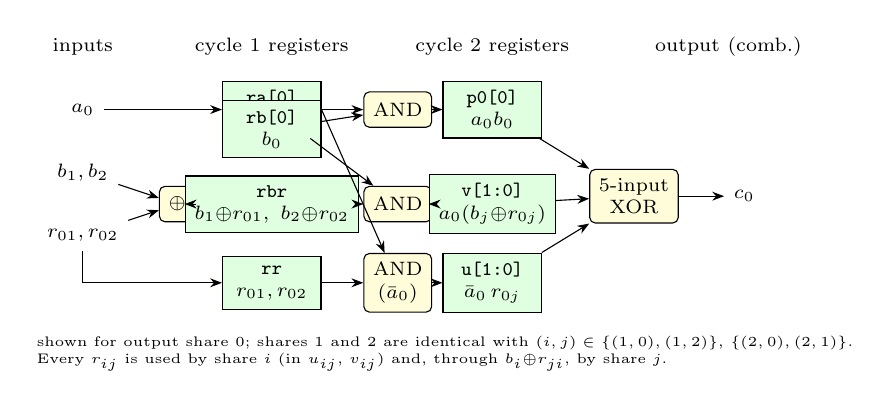
\begin{tikzpicture}[x=1cm,y=1cm,font=\scriptsize,>={Stealth[length=1.5mm]},
  r/.style={draw,fill=green!12,minimum width=1.25cm,minimum height=0.45cm,align=center},
  g/.style={draw,fill=yellow!15,rounded corners=2pt,minimum height=0.45cm,align=center}]
  \node at (0,2.3) {inputs}; \node at (2.4,2.3) {cycle 1 registers}; \node at (5.2,2.3) {cycle 2 registers}; \node at (8.2,2.3) {output (comb.)};
  \node (a) at (0,1.5) {$a_0$}; \node (b) at (0,0.7) {$b_1, b_2$}; \node (rin) at (0,-0.1) {$r_{01}, r_{02}$};
  \node[r] (ra) at (2.4,1.5) {\sig{ra[0]}\\$a_0$};
  \node[g] (xr) at (1.2,0.3) {$\oplus$};
  \node[r] (rbr) at (2.4,0.3) {\sig{rbr}\\$b_1{\oplus}r_{01},\ b_2{\oplus}r_{02}$};
  \node[r] (rr) at (2.4,-0.7) {\sig{rr}\\$r_{01}, r_{02}$};
  \node[r] (rb) at (2.4,2.25-1.0) {\sig{rb[0]}\\$b_0$};
  \node[g] (pa) at (4.0,1.5) {AND}; \node[r] (p) at (5.2,1.5) {\sig{p0[0]}\\$a_0 b_0$};
  \node[g] (va) at (4.0,0.3) {AND}; \node[r] (v) at (5.2,0.3) {\sig{v[1:0]}\\$a_0(b_j{\oplus}r_{0j})$};
  \node[g] (ua) at (4.0,-0.7) {AND\\($\bar a_0$)}; \node[r] (u) at (5.2,-0.7) {\sig{u[1:0]}\\$\bar a_0\, r_{0j}$};
  \node[g] (xo) at (7.0,0.4) {5-input\\XOR}; \node (c) at (8.4,0.4) {$c_0$};
  \draw[->] (a) -- (ra); \draw[->] (b) -- (xr); \draw[->] (rin) -- (xr); \draw[->] (xr) -- (rbr); \draw[->] (rin) |- (rr);
  \draw[->] (ra) -- (pa); \draw[->] (rb) -- (pa); \draw[->] (pa) -- (p);
  \draw[->] (ra) -- (va); \draw[->] (rbr) -- (va); \draw[->] (va) -- (v);
  \draw[->] (ra.east) -- (ua); \draw[->] (rr) -- (ua); \draw[->] (ua) -- (u);
  \draw[->] (p) -- (xo); \draw[->] (v) -- (xo); \draw[->] (u) -- (xo); \draw[->] (xo) -- (c);
  \node[font=\tiny,align=left] at (4.6,-1.6) {shown for output share 0; shares 1 and 2 are identical with $(i,j) \in \{(1,0),(1,2)\}$, $\{(2,0),(2,1)\}$.\\ Every $r_{ij}$ is used by share $i$ (in $u_{ij}$, $v_{ij}$) and, through $b_i{\oplus} r_{ji}$, by share $j$.};
\end{tikzpicture}
\caption{HPC2 gadget structure for output share 0 (conceptual, reconstructed from \file{pams\_jqr.v} lines 4--19). Two register layers separate the refresh $b_j \oplus r_{ij}$ from the cross products, so no glitch combines two shares.}\label{fig:hpc2}
\end{figure}

\begin{figure}[p]\centering
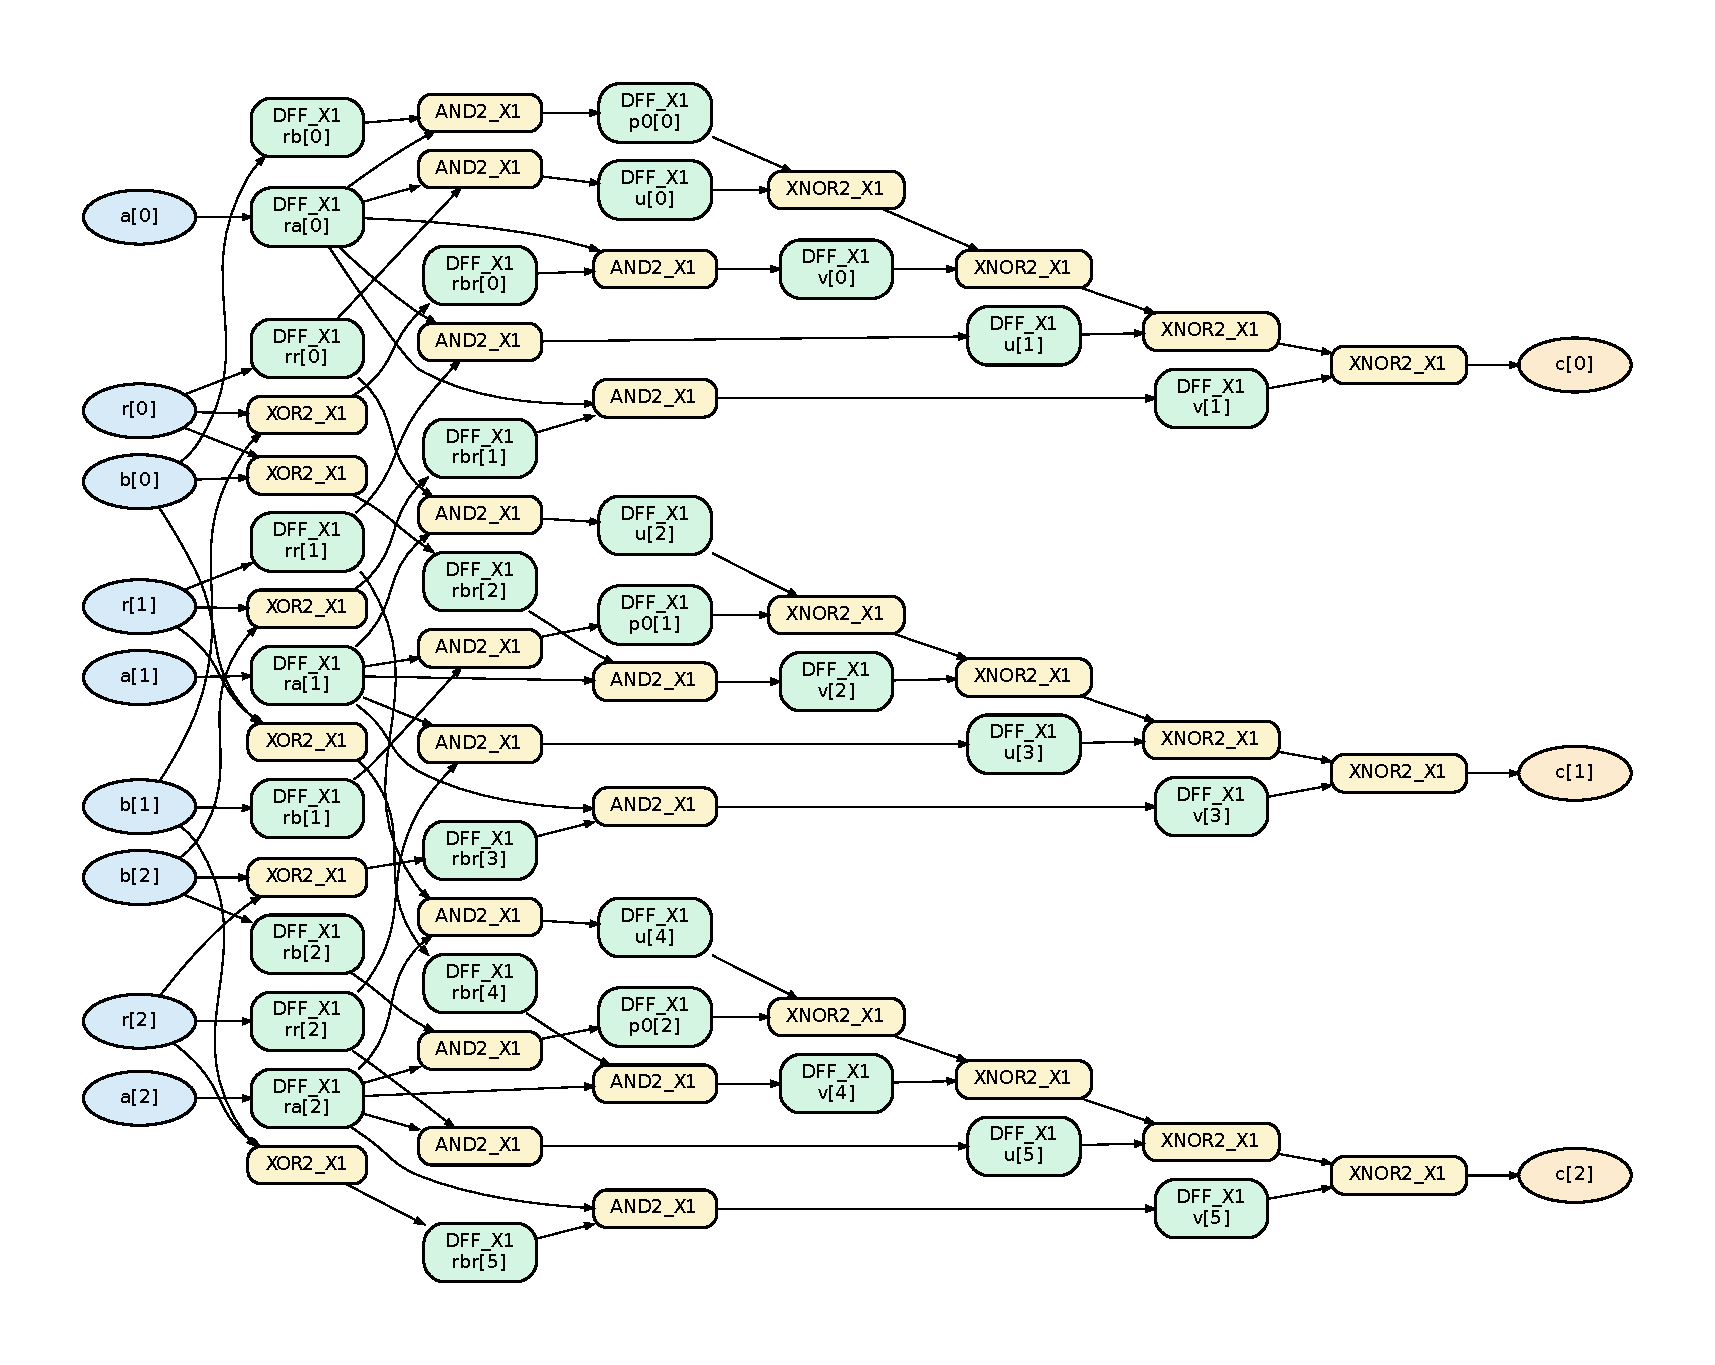
\includegraphics[width=0.92\textwidth]{figures/gates/hpc2_mapped.pdf}
\caption{The actual mapped HPC2 gadget (variant v0) from \file{competitors/runs/syn\_pams\_jqr\_p0/mapped.json}: every cell and every connection of module \sig{hpc2} after Yosys/ABC mapping to Nangate45, drawn automatically with Graphviz (\file{paper/scripts/generate\_figures.py}). Green = flip-flops, labelled with their RTL register names; yellow = combinational cells; ellipses = gadget ports. Clock connections are omitted.}\label{fig:hpc2-mapped}
\end{figure}

\subsection{Pipeline and critical paths}\label{app:critpath}
\paragraph{Stage structure.} \Cref{tab:v-stages} gives the stages. Every stage boundary is a register, and every combinational path runs between two registers of adjacent stages, or from a register to the outputs \sig{cdec}/\sig{dec}.

\paragraph{Synthesis timing.} In synthesis STA (no wires), the worst register group of \sig{pams\_jqr} is the public \sig{lowrq} ($1.033\ns$ including setup). Close behind are the partial products \sig{ml0} ($1.016\ns$) and \sig{mh0} ($0.994\ns$), and the public \sig{qcr} ($0.925\ns$). The later share-wise stages have slack: \sig{s0p} needs $0.784\ns$ and \sig{y0} $0.620\ns$. In the baseline every share-wise stage needs about $1.0\ns$.

\paragraph{Routed critical path at 1.2\ns{} (seed 1).} From \file{timing.rpt}, on RCX parasitics with a propagated clock:
\begin{itemize}
  \item \emph{Launch.} The path starts at flip-flop \sig{\_8799\_}, whose Q is \sig{x1r[5]}, bit 5 of share 1 at stage 2. The clock arrives after $0.179\ns$ of clock-tree latency, and clock-to-Q takes $0.168\ns$.
  \item \emph{Logic.} It passes 21 combinational cells:
    \begin{itemize}
      \item eight cells (\sig{XOR2}, \sig{NOR2}, \sig{OAI21}, \sig{AND2}, \sig{XNOR2}, \sig{XOR2}, \sig{XNOR2}, \sig{NOR2}) forming the carry-save part of the constant multiplication;
      \item twelve AOI/OAI-type cells (\sig{AOI21}, \sig{OAI221}, \sig{AOI221}, \sig{OAI21}, \sig{NAND2}, then alternating \sig{AOI21}/\sig{OAI21}), the carry propagation of the partial-product adder;
      \item a final \sig{XOR2\_X1} for the sum bit.
    \end{itemize}
  \item \emph{Capture.} It ends at the D pin of \sig{\_8676\_}, whose Q is \sig{ml1[23]}, bit 23 of the low partial product of share 1. The data arrives at $1.236\ns$. The required time is $1.343\ns$ ($1.2\ns$ + capture clock latency $0.180\ns$ $-$ setup $0.037\ns$), so the slack is $+0.107\ns$.
\end{itemize}
The baseline's path, \sig{x0r[9]}$\to$\sig{mh0[31]}, is the corresponding partial product of its 34-bit constant, with a $1.073\ns$ data path and slack $+0.089\ns$. Neither design's critical path involves a gadget or the masked kernel.

\subsection{Physical placement and routing}\label{app:physical}
\Cref{fig:layout} shows the routed layouts as rendered by OpenROAD's own GUI renderer (\texttt{save\_image}, run headless). Both images use the same resolution, $0.1\,\si{\micro\meter}$ per pixel, downsampled by 2 for the document, so their sizes compare directly:
\begin{itemize}
  \item \PAMS{}: die $188.7\,\si{\micro\meter}$ wide, $2075 \times 2075$ pixels at full resolution;
  \item baseline: die $209.0\,\si{\micro\meter}$, $2299 \times 2299$ pixels.
\end{itemize}
What the renders show:
\begin{itemize}
  \item the horizontal power-grid straps (pink) and vertical straps;
  \item signal wiring on metal 2 and metal 3 (red/green; most of the wire length);
  \item the I/O pins on the boundary;
  \item the standard cells underneath.
\end{itemize}
Functional regions cannot be read from such a render. \Cref{fig:placement} therefore colours the same cells by class using the DEF.

\begin{figure}[h]\centering
\begin{subfigure}[t]{0.47\textwidth}\centering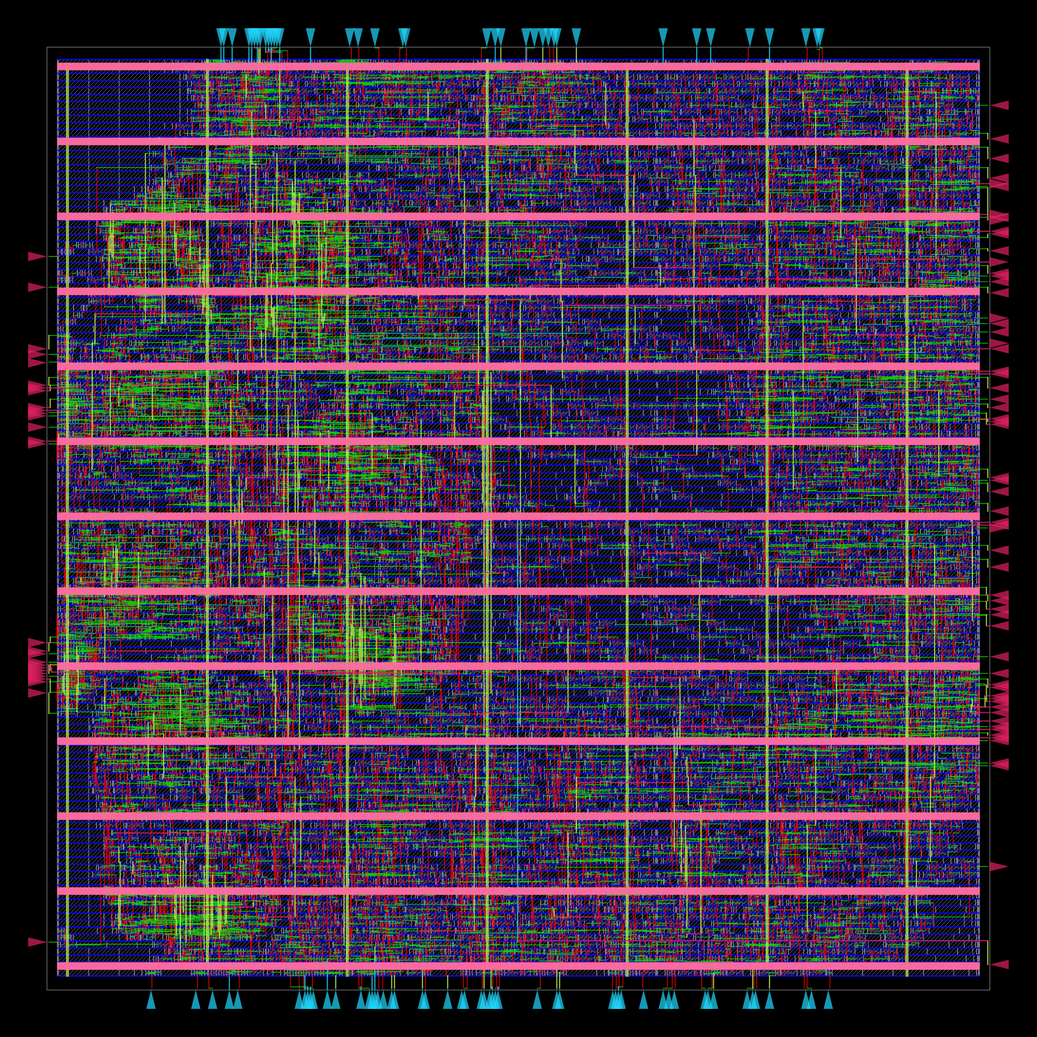
\includegraphics[width=0.903\linewidth]{figures/physical/layout_pams_jqr_half.png}\caption{\PAMS{} (\sig{pams\_jqr}), die $188.7^2\,\si{\micro\meter\squared}$}\end{subfigure}\hfill
\begin{subfigure}[t]{0.47\textwidth}\centering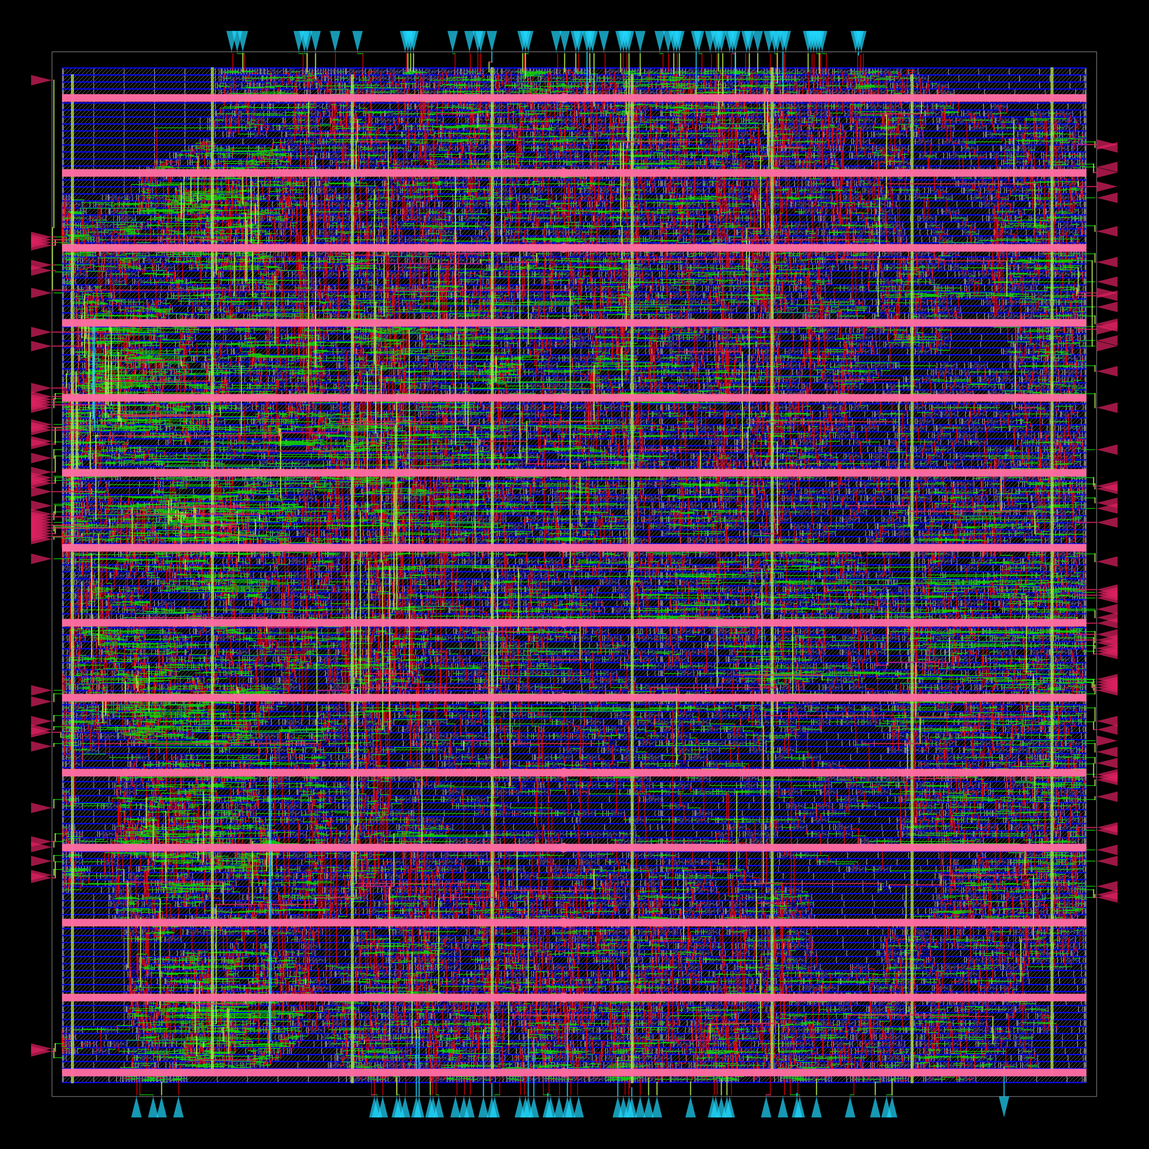
\includegraphics[width=\linewidth]{figures/physical/layout_base_jq_half.png}\caption{baseline (\sig{base\_jq}), die $209.0^2\,\si{\micro\meter\squared}$}\end{subfigure}
\caption{Routed layouts (target 1.2\ns, seed 1, utilization 50\,\%), rendered by OpenROAD (\texttt{save\_image}, $0.1\,\si{\micro\meter}$/pixel, downsampled $\times 2$) and shown at the same scale: the \PAMS{} image is $188.7/209.0 = 0.903$ of the baseline's width.}\label{fig:layout}
\end{figure}

\paragraph{Tool evidence for routability.} We do not infer congestion from appearance; \cref{tab:route-evidence} lists what the tools report.
\begin{itemize}
  \item \textbf{Detailed routing at 1.1\ns.} The router clears \PAMS{}'s initial violations in four iterations ($892 \to 98 \to 94 \to 0$). For baseline seed 2 it reaches 3 violations after three iterations and then oscillates between 2 and 11 violations for 50 further "stubborn tiles" iterations, ending at 3.
  \item \textbf{Hold buffering.} Hold fixing, which with I/O at the clock edge is the dominant source of buffers, inserts about 430--460 more buffers for the baseline. Its 3,210 clock sinks against 2,494 for \PAMS{} also make the clock tree larger.
\end{itemize}

\begin{table}[h]\centering\small
\caption{OpenROAD-reported routing quantities of representative runs.}\label{tab:route-evidence}
\begin{tabular}{@{}lrrrrr@{}}
\toprule
run & clock sinks & hold buffers & routed wire (\si{\micro\meter}) & DR iterations & final DRC \\
\midrule
\PAMS{} 1.2\ns{} s1 & 2,494 & 1,381 & 58,126 & 5 & 0 \\
baseline 1.2\ns{} s1 & 3,210 & 1,841 & 72,887 & 6 & 0 \\
\PAMS{} 1.1\ns{} s2 & 2,494 & 1,421 & 58,506 & 4 & 0 \\
baseline 1.1\ns{} s2 & 3,210 & 1,849 & 73,132 & 53 & 3 \\
baseline 1.1\ns{} s5 & 3,210 & 1,850 & 72,529 & 4 & 0 \\
\bottomrule
\end{tabular}
\end{table}

\subsection{Resource accounting}\label{app:resources}
\paragraph{How each count was obtained.}
\begin{itemize}
  \item \emph{Gadgets.} HPC2 instances in the RTL: 40 / 57. Synthesis and P\&R preserve them one-to-one (the G-check matches each routed gadget to the reference).
  \item \emph{Randomness.} The \sig{rnd} width: 3 bits per gadget, 120 / 171. The R-check verifies that each bit reaches exactly one gadget.
  \item \emph{Flip-flops.} \sig{DFF\_X1} count: 1,294 / 1,500 top-level plus 30 per gadget, i.e.\ 2,494 / 3,210 in total. These are also the clock sinks reported by CTS.
  \item \emph{Areas.} Liberty cell areas summed (synthesis) or OpenROAD \texttt{design\_area} (routed).
\end{itemize}

\paragraph{Functional decomposition.} \Cref{tab:resources-full} decomposes the synthesized area (\file{paper/scripts/resources.py}). Gadget cells are counted inside their hierarchy. Flip-flops are classified by the RTL name on their Q net. Every other combinational cell is assigned to the register group that its fan-out cone reaches first, and to "shared" if it reaches several. The decomposition sums exactly to the reported synthesis area, but the attribution of individual combinational cells is approximate where ABC shared logic between groups.

\begin{table}[h]\centering\small
\caption{Synthesized area by function, mapping 0 (cells, \si{\micro\meter\squared}).}\label{tab:resources-full}
\begin{tabular}{@{}lrrrr@{}}
\toprule
group & \multicolumn{2}{c}{\PAMS{}} & \multicolumn{2}{c}{baseline} \\
 & cells & area & cells & area \\
\midrule
HPC2 gadgets (63 cells / $180.35\um$ each) & 2,520 & 7,213.9 & 3,591 & 10,279.8 \\
FF: alignment (delay chains) & 782 & 3,536.2 & 876 & 3,961.3 \\
FF: partial products & 159 & 719.0 & 197 & 890.8 \\
FF: $x_r$, switched value, Yosys-named & 80 & 361.8 & 115 & 520.0 \\
FF: aligned operands $y_i$ & 42 & 189.9 & 72 & 325.6 \\
FF: public constants & 83 & 375.3 & 86 & 388.9 \\
FF: inputs, control, accumulator & 148 & 669.3 & 154 & 696.4 \\
logic $\to$ partial products & 1,972 & 2,274.0 & 1,968 & 2,406.0 \\
logic $\to$ switched value / Yosys-named & 305 & 335.7 & 444 & 626.7 \\
logic $\to$ aligned operands & 87 & 104.0 & 334 & 501.4 \\
logic $\to$ public constants & 783 & 961.3 & 70 & 75.0 \\
logic $\to$ gadget-input XOR network & 162 & 256.4 & 181 & 266.3 \\
logic $\to$ alignment, other, shared & 17 & 25.3 & 121 & 158.8 \\
\midrule
total & 7,140 & 17,022.1 & 8,209 & 21,097.0 \\
\bottomrule
\end{tabular}
\end{table}

\section{Extended Security and Experimental Evidence}\label{app:evidence}

\subsection{Formal gadget verification (SILVER)}\label{app:silver}
\paragraph{Method.} SILVER~\cite{knichel2020silver} represents every wire of a gate-level netlist as a reduced ordered binary decision diagram over the input shares and random bits. It decides probing security, NI, SNI and PINI exactly, by checking statistical independence of every probe combination. With glitch-extension enabled (the robust model) it also covers glitches.

\paragraph{What was verified.}
\begin{itemize}
  \item \textbf{Inputs.} The verified objects are the mapped \sig{hpc2} modules extracted verbatim from the synthesized netlists, with only two edits: duplicate wire declarations removed, and SILVER port annotations added.
  \item \textbf{Variants.} Across all mappings of all designs, synthesis produced exactly two distinct mapped variants, identified by the SHA-256 of the module text:
  \begin{itemize}
    \item v0: 12 of the 15 earlier synthesis mappings and all final P\&R inputs;
    \item v1: one mapping of each design.
  \end{itemize}
  \item \textbf{Results.} Both variants are probing-, NI-, PINI- and uniformity-secure up to order 2 in the standard and robust models. SNI holds up to order 2 in the standard model but only order 1 in the robust model, which is consistent with HPC2's guarantee (PINI, not SNI).
\end{itemize}

\paragraph{Negative controls, all failing as required.}
\begin{itemize}
  \item the refresh $b_j \oplus r_{ij}$ left unregistered: robust PINI fails;
  \item one random bit reused for two pairs: every property fails;
  \item an output recombining two shares: every property fails.
\end{itemize}

\paragraph{Application to the final circuits.} \file{final/models/gadget\_identity.py} recomputes the module hash of every final netlist: 5 synthesis mappings and the P\&R input, for each of \sig{pams\_jqr}, \sig{base\_jq}, \sig{pams\_jpr} and \sig{base\_jp}. All 24 are v0 or v1.

\subsection{Composition-precondition and structural checks}\label{app:compcheck}
\paragraph{Checks.} \file{validation/structure/compcheck.py} loads a netlist, treats every gadget as a black box with ports $a[i]$, $b[i]$, $r[k]$, $c[i]$, and propagates share-domain labels: input $x_i$ and gadget output $c[i]$ belong to domain $i$. It then checks:
\begin{description}[style=nextline,leftmargin=1.2em]
  \item[D] No net outside a gadget depends on two share domains.
  \item[R] Every \sig{rnd} bit reaches only the $r$-port of exactly one gadget, with three distinct bits per gadget, and all bits are used.
  \item[P] Gadget input $a[i]$, $b[i]$ depends only on domain $i$ and public data.
  \item[O] Lane output share $i$ of \sig{cdec} and \sig{dec} is domain $i$.
  \item[G] For routed netlists only: after collapsing P\&R buffers and ignoring drive strength, every gadget instance equals the reference gadget cell by cell and pin by pin.
\end{description}

\paragraph{Negative controls.} Edited netlists are all detected:
\begin{itemize}
  \item exposed decision: D = 2;
  \item partial recombination: D = 1;
  \item mask reuse: R = 2;
  \item a deliberately leaky lane: D = 71, P = 8.
\end{itemize}

\paragraph{Final results.} Pass on all of the following:
\begin{itemize}
  \item the 5 synthesis mappings and the P\&R input of both finalists;
  \item all 40 routed netlists of the final place-and-route campaign, i.e.\ every finished run including the DRC-failing ones (\file{final/runs/routed\_check\_final.jsonl}), with 0 G mismatches.
\end{itemize}
The checker is home-made; it is not an established tool. Its role is limited to mechanizing the preconditions of a published theorem, and its negative controls show that it detects violations.

\subsection{PROLEAD configuration and complete results}\label{app:prolead}
\paragraph{Gadget campaign.} Settings:
\begin{itemize}
  \item PROLEAD v3.1.0, library = PROLEAD's NANG45 entry;
  \item order 2, transitions on, robust (non-relaxed) model, multivariate, clock cycles 1--6;
  \item four back-to-back executions; fixed group $(a, b) = (1,1), (0,1), (1,0), (1,1)$ against random; fresh $r$;
  \item $2^{22}$ simulations, \num{6984} probing sets.
\end{itemize}
Results: v0 max 4.58 (re-run 4.22), v1 4.17 (re-run 4.59), so no leakage. All three broken variants give $-\log_{10} p = \infty$.

\paragraph{Lane campaigns.} Settings:
\begin{itemize}
  \item \textbf{Simulation.} One simulation streams a 36-coefficient ciphertext: 18 coefficients at $d = 11$, then 18 at $d = 5$. The fixed group uses boundary-adjacent matching coefficients; fresh \sig{rnd} every cycle.
  \item \textbf{Probes.} Probes sit on flip-flop D-pin nets, gadget input nets and outputs; in the robust model every other wire's extended probe is a subset of these. The test is univariate (probes in the same cycle).
  \item \textbf{Minimization.} "Trivial" minimization removes only duplicate probing sets.
  \item \textbf{Fixture.} It generates the arithmetic sharing from uniform 32-bit words, at statistical distance below $2^{-20}$ from uniform per share, and is excluded from probing.
\end{itemize}

\Cref{tab:prolead-full} lists every lane run.

\begin{table}[h]\centering\small
\caption{All lane PROLEAD runs. "null" = median of the maximum $-\log_{10} p$ over the given number of independent sets without leakage.}\label{tab:prolead-full}
\resizebox{\textwidth}{!}{%
\begin{tabular}{@{}lllrrrrl@{}}
\toprule
netlist & variant & order, cycles & simulations & probing sets & max & null & outcome \\
\midrule
\sig{pams\_jqr} & self-test (one wrong $c$) & 1, 36 & \num{4096} & 994 & -- & -- & output check fails, as required \\
\sig{pams\_jqr} & frozen & 1, 1--72 & \num{1048576} & \num{71568} & 5.53 & 5.01 & confirm ($2^{22}$): 0.78 \\
\sig{pams\_jqr} & frozen & 2, 36 & \num{262144} & \num{493055} & 5.21 & 5.85 & confirm ($2^{22}$): 0.44 \\
\sig{pams\_jqr} & NC partial recombination & 2, 36 & \num{65536} & \num{494047} & 41.4 & 5.85 & \textbf{detected} \\
\midrule
frozen \sig{pams} & frozen & 1, 1--70 & \num{4194304} & \num{67130} & 4.47 & 4.99 & no flag \\
frozen \sig{pams} & frozen & 1, 34 & \num{65536} & 910 & 2.63 & 3.12 & no flag \\
frozen \sig{pams} & frozen & 2, 34 & \num{65536} & \num{459212} & 6.08 & 5.82 & confirm ($2^{22}$): 0.24 \\
frozen \sig{pams} & frozen & 2, 34 & \num{1048576} & \num{459212} & 5.96 & 5.82 & confirm ($2^{22}$): 1.81 \\
frozen \sig{base} & frozen & 1, 1--72 & \num{4194304} & \num{95976} & 5.46 & 5.14 & confirm ($2^{24}$): 1.59 \\
frozen \sig{base} & frozen & 2, 36 & \num{1048576} & \num{887642} & 6.79 & 6.11 & confirm ($2^{22}$): 1.20 \\
frozen \sig{pams} & NC exposed decision & 1, 31--36 & \num{65536} & \num{5760} & $\infty$ & 3.92 & \textbf{detected} \\
frozen \sig{pams} & NC partial recombination & 2, 34 & \num{65536} & \num{460169} & 48.9 & 5.82 & \textbf{detected} \\
frozen \sig{base} & NC partial recombination & 2, 36 & \num{65536} & \num{888973} & 22.5 & 6.11 & \textbf{detected} \\
frozen \sig{pams} & NC mask reuse & 2, 34 & \num{262144} & \num{458254} & $\infty$ & 5.82 & \textbf{detected} \\
\bottomrule
\end{tabular}}
\end{table}

\paragraph{Caveats.}
\begin{enumerate}
  \item PROLEAD~3.1.0 does not seed \texttt{rand()} in hardware mode. Confirmations therefore use a strictly larger simulation count, whose prefix equals the screening data. Rising evidence would indicate a leak; every confirmation instead decayed below 2.
  \item The probe sets for second order cover one steady-state cycle per lane, not every cycle pair.
  \item Statistical non-detection is not a proof.
  \item FLINT aborted some runs inside PROLEAD's evaluation: 1 of 10 gadget runs and 4 early lane runs. All were re-run, and no aborted run is counted.
\end{enumerate}

\subsection{Benchmark configuration}\label{app:config}
\paragraph{Synthesis.} \file{bfbench.py} (copied to \file{final/external/}), function \sig{synth}, with flow B:
\begin{itemize}
  \item \texttt{read\_verilog -sv}; \texttt{synth -top <lane> -flatten -noabc}; \texttt{dfflibmap -liberty <lib>};
  \item \texttt{abc -liberty <lib> -constr <BUF\_X1 drive, 5 fF load> -D 500}; \texttt{clean}; \texttt{stat}.
\end{itemize}
The five mappings vary $-D$ (400, 650) and add 3 or 6 unrelated pad modules. Synthesis area varies by at most 0.6\,\% across mappings for every design.

\paragraph{P\&R.} \file{final/tools/pnr\_final.tcl}, a copy of the earlier flow script with only the seed added.
\begin{itemize}
  \item \emph{Clock and I/O.} One clock on \sig{clk} at the target period; input delay 0 and output delay 0 relative to it; input transition 0.05\ns; output load 5\,fF; no clock uncertainty. Don't-use cells: \sig{TAPCELL\_X1}, \sig{FILLCELL\_X1}, \sig{AOI211\_X1}, \sig{OAI211\_X1}.
  \item \emph{Floorplan and placement.} Floorplan utilization 0.5, aspect 1, 2\,\si{\micro\meter} core space; tracks and tapcells from the platform; PDN grid M1--M4--M7. Global placement density 0.6 (wirelength-driven, then timing-driven) with \texttt{-random\_seed}; pins on metal5/metal6 with \texttt{-random\_seed}.
  \item \emph{Optimization and CTS.} \texttt{repair\_design}, \texttt{repair\_tie\_fanout}, detailed placement; CTS with root BUF\_X4 and buffers BUF\_X4/BUF\_X8 with sink clustering; \texttt{repair\_timing -setup}; \texttt{repair\_timing -hold -max\_buffer\_percent 60}.
  \item \emph{Routing.} Signal layers metal2--metal10, clock metal4--metal10, layer adjustment 0.5; global route with 50 congestion iterations; post-GRT setup repair; \texttt{detailed\_route -droute\_end\_iter 64}; fillers.
  \item \emph{Extraction.} RCX with the platform's \file{rcx\_patterns.rules}.
\end{itemize}

\subsection{Every P\&R run}\label{app:runs}
\Cref{tab:pnr-runs} lists all 42 runs. The critical path is the worst setup path in \file{timing.rpt}, given as the RTL names of its launch and capture registers.

\begin{table}[p]\centering\scriptsize
\caption{All 42 final P\&R runs (utilization 50\,\%, density 0.6), generated by \file{paper/scripts/tables.py} from \file{final/runs/pnr\_stats.json}. Status: valid (0 DRC, RCX, hold met), DRC $n$ (finished with $n$ violations), TIMEOUT (stopped at 90 min, no result).}\label{tab:pnr-runs}
\resizebox{\textwidth}{!}{\begin{tabular}{@{}llrlrrrrrrl@{}}
\toprule
design & target & seed & status & period (ns) & setup WNS & hold WNS & cell (\si{\micro\meter\squared}) & buffers & wire (\si{\micro\meter}) & critical path (launch$\to$capture) \\
\midrule
pams\_jqr & 2.0 & 1 & valid & 1.162 & +0.838 & +0.0070 & 18706 & 1524 & 58070 & e0r[2]$\to$lowrq[13] \\
pams\_jqr & 2.0 & 2 & valid & 1.156 & +0.844 & +0.0082 & 18718 & 1535 & 58066 & e0r[2]$\to$lowrq[13] \\
pams\_jqr & 2.0 & 3 & valid & 1.165 & +0.835 & +0.0075 & 18734 & 1546 & 57941 & e0r[2]$\to$lowrq[13] \\
pams\_jqr & 2.0 & 4 & valid & 1.161 & +0.839 & +0.0087 & 18771 & 1565 & 57879 & e0r[2]$\to$lowrq[13] \\
pams\_jqr & 2.0 & 5 & valid & 1.146 & +0.854 & +0.0090 & 18754 & 1562 & 57822 & e0r[2]$\to$lowrq[13] \\
pams\_jqr & 2.0 & 6 & valid & 1.153 & +0.847 & +0.0069 & 18740 & 1543 & 57946 & e0r[2]$\to$lowrq[13] \\
pams\_jqr & 2.0 & 7 & valid & 1.155 & +0.845 & +0.0055 & 18722 & 1530 & 57761 & e0r[2]$\to$lowrq[13] \\
base\_jq & 2.0 & 1 & valid & 1.222 & +0.778 & +0.0080 & 23290 & 2057 & 72122 & shp[0]$\to$y0[23] \\
base\_jq & 2.0 & 2 & valid & 1.234 & +0.766 & +0.0059 & 23266 & 2047 & 72306 & shp[1]$\to$y0[23] \\
base\_jq & 2.0 & 3 & valid & 1.142 & +0.858 & +0.0050 & 23284 & 2048 & 73196 & x0r[10]$\to$mh0[31] \\
base\_jq & 2.0 & 4 & valid & 1.158 & +0.842 & +0.0059 & 23273 & 2045 & 73208 & x0r[10]$\to$mh0[31] \\
base\_jq & 2.0 & 5 & valid & 1.255 & +0.745 & +0.0066 & 23286 & 2052 & 72709 & shp[0]$\to$y0[23] \\
base\_jq & 2.0 & 6 & valid & 1.198 & +0.802 & +0.0064 & 23285 & 2047 & 72622 & shp[1]$\to$y0[23] \\
base\_jq & 2.0 & 7 & valid & 1.193 & +0.807 & +0.0054 & 23309 & 2056 & 72244 & shp[1]$\to$y0[23] \\
pams\_jqr & 1.2 & 1 & valid & 1.093 & +0.107 & +0.0084 & 18742 & 1555 & 58126 & x1r[5]$\to$ml1[23] \\
pams\_jqr & 1.2 & 2 & valid & 1.091 & +0.109 & +0.0086 & 18710 & 1537 & 58000 & x1r[5]$\to$ml1[23] \\
pams\_jqr & 1.2 & 3 & valid & 1.094 & +0.106 & +0.0039 & 18750 & 1558 & 57943 & x1r[5]$\to$ml1[23] \\
pams\_jqr & 1.2 & 4 & valid & 1.093 & +0.107 & +0.0064 & 18778 & 1576 & 58065 & e0r[3]$\to$lowrq[13] \\
pams\_jqr & 1.2 & 5 & valid & 1.094 & +0.106 & +0.0079 & 18770 & 1584 & 58239 & x1r[5]$\to$ml1[23] \\
pams\_jqr & 1.2 & 6 & valid & 1.097 & +0.103 & +0.0087 & 18763 & 1572 & 58123 & e0r[2]$\to$lowrq[13] \\
pams\_jqr & 1.2 & 7 & valid & 1.097 & +0.103 & +0.0062 & 18734 & 1552 & 58075 & x1r[5]$\to$ml1[23] \\
base\_jq & 1.2 & 1 & valid & 1.111 & +0.089 & +0.0045 & 23278 & 2067 & 72887 & x0r[9]$\to$mh0[31] \\
base\_jq & 1.2 & 2 & valid & 1.109 & +0.091 & +0.0064 & 23296 & 2081 & 73184 & x0r[9]$\to$mh0[31] \\
base\_jq & 1.2 & 3 & valid & 1.103 & +0.097 & +0.0062 & 23334 & 2107 & 73585 & x0r[9]$\to$mh0[31] \\
base\_jq & 1.2 & 4 & valid & 1.104 & +0.096 & +0.0059 & 23338 & 2095 & 72906 & x2r[9]$\to$mh2[31] \\
base\_jq & 1.2 & 5 & valid & 1.102 & +0.098 & +0.0065 & 23282 & 2071 & 72891 & x0r[11]$\to$mh0[31] \\
base\_jq & 1.2 & 6 & valid & 1.109 & +0.091 & +0.0075 & 23304 & 2081 & 72887 & x1r[4]$\to$ml1[31] \\
base\_jq & 1.2 & 7 & valid & 1.105 & +0.095 & +0.0067 & 23314 & 2076 & 72912 & x2r[9]$\to$mh2[31] \\
pams\_jqr & 1.1 & 1 & valid & 1.068 & +0.032 & +0.0064 & 18779 & 1604 & 58366 & c0r[0]$\to$lowrq[13] \\
pams\_jqr & 1.1 & 2 & valid & 1.066 & +0.034 & +0.0089 & 18828 & 1650 & 58506 & c0r[0]$\to$lowrq[13] \\
pams\_jqr & 1.1 & 3 & valid & 1.067 & +0.033 & +0.0047 & 18786 & 1609 & 58402 & c0r[0]$\to$lowrq[13] \\
pams\_jqr & 1.1 & 4 & valid & 1.070 & +0.030 & +0.0061 & 18785 & 1591 & 58067 & c0r[0]$\to$lowrq[13] \\
pams\_jqr & 1.1 & 5 & valid & 1.062 & +0.038 & +0.0067 & 18777 & 1597 & 58381 & c0r[0]$\to$lowrq[13] \\
pams\_jqr & 1.1 & 6 & valid & 1.068 & +0.032 & +0.0065 & 18789 & 1602 & 58349 & c0r[0]$\to$lowrq[13] \\
pams\_jqr & 1.1 & 7 & valid & 1.068 & +0.032 & +0.0067 & 18794 & 1609 & 58431 & c0r[0]$\to$lowrq[12] \\
base\_jq & 1.1 & 1 & TIMEOUT & -- & -- & -- & -- & -- & 72866 & --$\to$-- \\
base\_jq & 1.1 & 2 & DRC 3 & 1.069 & +0.031 & +0.0073 & 23343 & 2126 & 73132 & mh1[9]$\to$fq1[22] \\
base\_jq & 1.1 & 3 & DRC 1 & 1.073 & +0.027 & +0.0065 & 23384 & 2164 & 72650 & ml1[16]$\to$fq1[23] \\
base\_jq & 1.1 & 4 & DRC 6 & 1.072 & +0.028 & +0.0061 & 23394 & 2172 & 73494 & x2r[9]$\to$mh2[31] \\
base\_jq & 1.1 & 5 & valid & 1.066 & +0.034 & +0.0083 & 23367 & 2136 & 72529 & mh0[9]$\to$fq0[22] \\
base\_jq & 1.1 & 6 & TIMEOUT & -- & -- & -- & -- & -- & 73381 & --$\to$-- \\
base\_jq & 1.1 & 7 & DRC 3 & 1.072 & +0.028 & +0.0064 & 23344 & 2117 & 73169 & mh0[9]$\to$fq0[23] \\
\bottomrule
\end{tabular}
}
\end{table}

\paragraph{Variation statistics} (valid runs; from \file{final/runs/pnr\_stats.json}):
\begin{itemize}
  \item \emph{Period standard deviation:} \PAMS{} 0.007 / 0.002 / 0.002\ns{} at 2.0 / 1.2 / 1.1\ns{}; baseline 0.041 / 0.003\ns{} (one valid run at 1.1).
  \item \emph{Cell-area standard deviation:} 22 / 23 / 17\um{} (\PAMS{}) and 14 / 24\um{} (baseline).
  \item \emph{Rank-sum $p$ (cell area):} 0.0006 at 2.0 and 1.2\ns{}.
  \item \emph{Rank-sum $p$ (period):} 0.073 (2.0\ns) and 0.0006 (1.2\ns).
\end{itemize}

\paragraph{Failed and stopped runs.}
\begin{itemize}
  \item All are baseline runs at 1.1\ns: seeds 2, 3, 4 and 7 finished with 3, 1, 6 and 3 DRC violations. Their periods (1.069--1.073\ns) are reported but not used.
  \item Seeds 1 and 6 were stopped at the 90-minute limit, after 126 and 90 minutes; seed 1 was then 40\,\% through a stubborn-tiles iteration with 13 violations.
  \item No \PAMS{} run failed.
  \item One campaign launch failed before running anything (a shell quoting error) and was relaunched from a script file.
\end{itemize}

\subsection{Functional verification}\label{app:functional}
\begin{table}[h]\centering\small
\caption{Functional verification of the final circuits (0 mismatches everywhere).}\label{tab:functional}
\resizebox{\textwidth}{!}{%
\begin{tabular}{@{}lllrr@{}}
\toprule
netlist & level & stimulus & coefficients & ciphertexts (accepting) \\
\midrule
\sig{pams\_jqr}, \sig{base\_jq}, \sig{pams}, \sig{base} & RTL & systematic & \num{39112} each & \num{7096} (76) \\
\sig{pams\_jqr}, \sig{base\_jq} & gate (mapping 0, P\&R input) & systematic & \num{39112} each & \num{7096} (76) \\
\sig{pams\_jqr}, \sig{base\_jq} & routed (\file{final.v}, 2.0\ns{} target, seed 1) & systematic + random & \num{39112} + \num{6001} & \num{7096} + \num{1086} (573) \\
\sig{pams\_jqr}, \sig{base\_jq} & RTL + 5 gate mappings & random & \num{6001} + $5 \times$ \num{1500} & \num{1079} (558) \\
\bottomrule
\end{tabular}}
\end{table}
The systematic stimulus (\file{final/models/fsim.py}) covers:
\begin{itemize}
  \item every interval boundary of every $(c, d)$;
  \item every $x \in [0, q)$ for every $d$, against $c = \Comp(x)$ and $c + 1$;
  \item share patterns rotating over random, $(x, 0, 0)$, $(0, x, 0)$, $(0, 0, x)$, $(q-1, q-1, x+2)$ and $(r, q - 1, \cdot)$.
\end{itemize}
The random stimulus is the frozen \file{models/sim.py}.

\subsection{Competitor study}\label{app:competitors}
\Cref{tab:competitors} lists the matched synthesis results of every design built in the competitor study (median of 5 mappings).
\begin{itemize}
  \item \textbf{Suffixes.}
  \begin{itemize}
    \item \sig{j}: just-in-time operands;
    \item \sig{p}/\sig{q}: one/two extra front-end stages;
    \item \sig{r}: \PAMS{} public retiming;
    \item \sig{bk}: Brent--Kung carry;
    \item \sig{hoc}: HOCompress precision;
    \item \sig{bos}: Bos-style interval check.
  \end{itemize}
  \item \textbf{Coron et al.'s arithmetic zero test.} It was bounded rather than built. An exact path for $d = 10/11$ needs at least three masked mod-$q$ multiplications per coefficient, i.e.\ at least 27 partial products of $12 \times 12$ bits. One unmasked registered $12 \times 12$ multiplier synthesizes to $1{,}241\um$ under the same flow, so at least $33{,}500\um$ for the multipliers alone, about twice the whole \PAMS{} lane.
  \item \textbf{Excluded.} Probabilistic comparisons (random linear combinations) are excluded because they are not exact.
\end{itemize}

\begin{table}[h]\centering\small
\caption{Competitor study, synthesis (Nangate45, flow B, median of 5 mappings), generated from \file{competitors/runs/cbench.json}.}\label{tab:competitors}
\begin{tabular}{@{}lrrrrrrl@{}}
\toprule
design & area (\si{\micro\meter\squared}) & delay (ns) & FFs (top) & HPC2 & rnd bits & latency & checks (gate / domain / composition) \\
\midrule
base & 21{,}598 & 1.649 & 1{,}565 & 57 & 171 & 31+4 & pass/pass/pass \\
pams & 16{,}998 & 1.487 & 1{,}309 & 40 & 120 & 29+4 & pass/pass/pass \\
base\_j & 19{,}915 & 1.646 & 1{,}171 & 57 & 171 & 31+4 & pass/pass/pass \\
base\_p & 21{,}940 & 1.388 & 1{,}665 & 57 & 171 & 32+4 & pass/pass/pass \\
base\_jp & 20{,}048 & 1.457 & 1{,}271 & 57 & 171 & 32+4 & pass/pass/pass \\
base\_bk & 20{,}731 & 1.715 & 711 & 75 & 225 & 17+4 & pass/pass/pass \\
base\_bkp & 21{,}019 & 1.512 & 811 & 75 & 225 & 18+4 & pass/pass/pass \\
hoc & 22{,}583 & 1.773 & 1{,}744 & 59 & 177 & 33+4 & pass/pass/pass \\
hoc\_jp & 20{,}948 & 1.438 & 1{,}381 & 59 & 177 & 34+4 & pass/pass/pass \\
bos & 28{,}604 & 1.642 & 2{,}171 & 91 & 273 & 31+4 & pass/pass/pass \\
bos\_j & 26{,}843 & 1.633 & 1{,}777 & 91 & 273 & 31+4 & pass/pass/pass \\
base\_q & 22{,}753 & 1.080 & 1{,}894 & 57 & 171 & 33+4 & pass/pass/pass \\
base\_jq & 21{,}097 & 1.057 & 1{,}500 & 57 & 171 & 33+4 & pass/pass/pass \\
hoc\_jq & 21{,}820 & 1.116 & 1{,}610 & 59 & 177 & 35+4 & pass/pass/pass \\
pams\_j & 15{,}812 & 1.565 & 1{,}041 & 40 & 120 & 29+4 & pass/pass/pass \\
pams\_p & 17{,}349 & 1.306 & 1{,}379 & 40 & 120 & 30+4 & pass/pass/pass \\
pams\_jp & 16{,}207 & 1.234 & 1{,}111 & 40 & 120 & 30+4 & pass/pass/pass \\
pams\_jpr & 16{,}237 & 1.163 & 1{,}107 & 40 & 120 & 30+4 & pass/pass/pass \\
pams\_q & 18{,}133 & 1.212 & 1{,}566 & 40 & 120 & 31+4 & pass/pass/pass \\
pams\_jq & 16{,}997 & 1.242 & 1{,}298 & 40 & 120 & 31+4 & pass/pass/pass \\
pams\_jqr & 17{,}022 & 1.033 & 1{,}294 & 40 & 120 & 31+4 & pass/pass/pass \\
\bottomrule
\end{tabular}

\end{table}

\subsection{Full cross-layer traceability}\label{app:traceability}
\Cref{tab:trace} connects each operation from equation to measured cost. Gate-level regions are identified by register names, which survive synthesis, and by gadget instances. Combinational logic between registers is identified only as the fan-in cone of those registers, because synthesis restructures it.

\begin{table}[h]\centering\scriptsize
\caption{Cross-layer traceability (concise version in \cref{tab:map}; extended discussion in \file{paper/CROSS\_LAYER\_TRACEABILITY.md}).}\label{tab:trace}
\setlength{\tabcolsep}{3pt}
\begin{tabularx}{\textwidth}{@{}R{2.1cm}R{1.6cm}R{1.4cm}R{2.4cm}YR{0.8cm}R{1.7cm}R{1.9cm}@{}}
\toprule
operation & equation & Verilog lines & RTL signals & gate-level region (synthesized / routed) & stage & figure & cost (synthesis) \\
\midrule
arithmetic-share input & \cref{eq:target} & 21--26, 42--43 & \sig{x$i$}, \sig{x$i$q}, \sig{x$i$r} & 72 \sig{DFF\_X1} (Q = \sig{x$i$q}, \sig{x$i$r}) & 1--2 & \cref{fig:datapath} & $326\um$ \\
share-wise modulus switch & \cref{eq:yi} & 48--54 & \sig{mh$i$}, \sig{ml$i$}, \sig{m$i$}, \sig{s$i$p} & fan-in cones of \sig{mh$i$}/\sig{ml$i$}/\sig{s$i$p} registers (XOR/XNOR trees, AOI/OAI carry chains); orange cells in \cref{fig:placement}; routed critical path at 1.2\ns{} & 3--4 & \cref{fig:datapath,fig:placement,fig:critpath} & $3{,}528\um$ (regs + logic, 3 shares) \\
public anchor & \cref{eq:low} & 31--44, 48--54 & \sig{qc}, \sig{qcr}, \sig{e0r}, \sig{c0r}, \sig{lowr}, \sig{lowrq}, \sig{lowp} & fan-in cones of \sig{qcr}/\sig{lowrq}/\sig{lowp}; routed critical path at 2.0 and 1.1\ns{} & 2--4 & \cref{fig:datapath} & \multirow{2}{2cm}{$1{,}337\um$ (both, regs + logic)} \\
public threshold & \cref{eq:thetaclosed} & 39--40, 45, 48--56 & \sig{qn}, \sig{qnr}, \sig{thr}, \sig{thrq}, \sig{thp}, \sig{th2} & fan-in cones of \sig{qnr}/\sig{thrq}/\sig{thp}/\sig{th2} & 2--5 & \cref{fig:datapath} & \\
corrected share combination & \cref{eq:y0} & 56 & \sig{y0}, \sig{y1}, \sig{y2} & 42 \sig{DFF\_X1} (Q = \sig{y$i$}) + subtract logic on share 0 & 5 & \cref{fig:datapath} & $294\um$ \\
protected comparison (CSA, ripple, comparator, zero test) & \cref{eq:Z,eq:b} & 58--1537 & \sig{ug111}--\sig{ug1542}, \sig{x$N$}, \sig{r$N$} & 38 \sig{hpc2} instances (exact boundary), 782 delay \sig{DFF\_X1}, 162 share-local XOR/XNOR cells at gadget inputs; blue/green cells in \cref{fig:placement} & 5--31 & \cref{fig:slice,fig:placement} & $6{,}853 + 3{,}558 + 256\um$ \\
HPC2 nonlinear operation & -- & 4--19 & \sig{ra}, \sig{rb}, \sig{rr}, \sig{rbr}, \sig{p0}, \sig{u}, \sig{v} & 63 cells per instance: 30 DFF, 15 AND2, 6 XOR2, 12 XNOR2 & 2 cycles & \cref{fig:hpc2,fig:hpc2-mapped} & $180.35\um$ each \\
ciphertext accumulation & \cref{eq:pred} & 2730--2746 & \sig{uacc}, \sig{ufin}, \sig{acc\_last}, \sig{vp}/\sig{fp}/\sig{lp} & 2 \sig{hpc2} + 3 DFF + control shift registers & 31--35 & \cref{fig:datapath} & $361 + 457\um$ \\
\bottomrule
\end{tabularx}
\end{table}

\subsection{Figure provenance}\label{app:provenance}
\Cref{tab:provenance} classifies every figure by how it was made. "Conceptual" figures were drawn by hand in TikZ from the RTL and are not extracted circuits.

\begin{table}[h]\centering\scriptsize
\caption{Provenance of every figure (details in \file{paper/FIGURE\_PROVENANCE.md}).}\label{tab:provenance}
\setlength{\tabcolsep}{3pt}
\begin{tabularx}{\textwidth}{@{}R{2.4cm}YYR{1.6cm}R{2.2cm}@{}}
\toprule
figure & source artifact & extraction method & design & type \\
\midrule
\cref{fig:boundaries} & \file{models/\allowbreak pams.py} (reference functions) & \file{generate\_figures.py} \sig{fig\_math}, matplotlib & math & graph from data \\
\cref{fig:datapath} & \file{final/\allowbreak rtl/\allowbreak pams\_jqr.v} & hand-drawn TikZ from source inspection & \sig{pams\_jqr} & conceptual \\
\cref{fig:slice} & \file{competitors/\allowbreak runs/\allowbreak syn\_pams\_jqr\_p0/\allowbreak mapped.json} & fan-in extraction (\sig{dot\_slice}), Graphviz & \sig{pams\_jqr} & extracted gate level \\
\cref{fig:placement} & \file{final/\allowbreak runs/\allowbreak pnr\_\{pams\_jqr,base\_jq\}\_T1.2\_s1/\allowbreak final.def}, \file{timing.rpt}; LEF sizes & DEF parsing (\sig{fig\_placement}), matplotlib & both & physical (EDA data) \\
\cref{fig:domains} & architecture and composition argument & hand-drawn TikZ & -- & conceptual \\
\cref{fig:area,fig:die,fig:timing,fig:gadgets,fig:random,fig:adp,fig:routing} & \file{final/\allowbreak runs/\allowbreak pnr\_stats.json}, \file{competitors/\allowbreak runs/\allowbreak cbench.json}, \file{final/\allowbreak data/\allowbreak gadget\_breakdown.csv} & \file{generate\_figures.py}, matplotlib & both & graphs from data \\
\cref{fig:critpath} & \file{final/\allowbreak runs/\allowbreak pnr\_*\_T1.2\_s1/\allowbreak timing.rpt}, \file{final.v} & report parsing (\sig{fig\_critpath}) & both & timing data \\
\cref{fig:hpc2} & \file{pams\_jqr.v} lines 4--19 & hand-drawn TikZ & \sig{hpc2} & conceptual \\
\cref{fig:hpc2-mapped} & \file{competitors/\allowbreak runs/\allowbreak syn\_pams\_jqr\_p0/\allowbreak mapped.json} (module \sig{hpc2}) & full module export (\sig{dot\_hpc2}), Graphviz & \sig{hpc2} v0 & extracted gate level \\
\cref{fig:layout} & \file{final/\allowbreak runs/\allowbreak pnr\_\{pams\_jqr,base\_jq\}\_T1.2\_s1/\allowbreak final.def} + platform LEF & OpenROAD \texttt{save\_image} (headless) & both & EDA layout export \\
\bottomrule
\end{tabularx}
\end{table}

\subsection{Reproduction and artifact identifiers}\label{app:repro}
\paragraph{Commands.} Exact commands, with pinned versions (Ubuntu 24.04.4, Python 3.12.3, Yosys 0.33, Icarus Verilog 12.0, OpenSTA 3.1.0, OpenROAD from ORFS 26Q3-705-gecb3cfdeb, PROLEAD 3.1.0, TinyTeX/TeX Live 2026 for this paper), are in \file{final/FINAL\_REPRODUCIBILITY.md}. The main results reproduce with:
\begin{lstlisting}[language=bash,numbers=none,basicstyle=\ttfamily\scriptsize]
python3 -I validation/math/audit.py                 # exactness (checks A-G)
bash final/models/fsim_all.sh                       # RTL + gate-level functional checks
python3 -I final/models/gadget_identity.py          # gadgets == SILVER-verified variants
bash final/tools/campaign1.sh                       # 42 seeded P&R runs (with final/tools/watchdog.sh)
python3 -I final/models/pnr_stats.py                # statistics
bash paper/scripts/build.sh -f                      # all paper figures, tables and this PDF
\end{lstlisting}

\paragraph{Identifiers.} SHA-256 of \sig{pams\_jqr.v}: \texttt{804fd73a263baacb371033015171519213d84cfa817dee9ba6ae2b3760ba0e7f}; of \sig{base\_jq.v}: \texttt{e573286a2b1b4ead019699538be21b454bab359fdaeb4f62e273d137458f6533}. Further hashes are in \file{final/PUBLICATION\_MANIFEST.md} of the public repository.

\end{document}
